\documentclass[a4paper,oneside,12pt]{book}
%----------------------------------------------------------------------------------------
%	WELCOME!
%   It's probably worth having a read through this file to set up the broad parameters.
%----------------------------------------------------------------------------------------

%----------------------------------------------------------------------------------------
%	COVER PAGE
%   The cover page is laid out in title/title.tex. You can choose a colour
%   or black and white logo
%----------------------------------------------------------------------------------------

%----------------------------------------------------------------------------------------
%	THESIS INFORMATION
%   Put title, author name, degree, type of work, school, department in here
%   It will be used for the title page and for the embedded PDF information
%----------------------------------------------------------------------------------------
\newcommand\YUGE{\fontsize{70}{84}\selectfont}
%\newcommand{\thesistitle}{EVEREST} % Your thesis title, this is used in the title and abstract
%\newcommand{\subtitlethesis}{Earth Visco-Elastic anisotRopic propErties SimulaTor} %
%\newcommand{\subtitlethesis}{Exploring Visco-Elastic anisotRopiES in the manTle} %
\newcommand{\thesistitle}{\textbf{ECOMAN}} % Your thesis title, this is used in the title and abstract
%\newcommand{\subtitlethesis}{Earth Visco-Elastic anisotRopic propErties SimulaTor} %
\newcommand{\subtitlethesis}{Exploring the COnsequences of Mechanical \\Anisotropy in the maNtle} %
\newcommand{\typeofthesis}{User Manual - Version 2.0} % dissertation, Final Year Project, report, etc.
%\author[1]{Manuele Faccenda (\href{mailto:manuele.faccenda@unipd.it} {manuele.faccenda@unipd.it})}
%\author[2]{Brandon P. VanderBeek (\href{mailto:brandonpaul.vanderbeek@unipd.it} {brandonpaul.vanderbeek@unipd.it})}
\newcommand{\authorname}{Manuele Faccenda (\href{mailto:manuele.faccenda@unipd.it} {manuele.faccenda@unipd.it}) \\ 
Brandon P. VanderBeek (\href{mailto:brandonpaul.vanderbeek@unipd.it} {brandonpaul.vanderbeek@unipd.it}) \\
Albert de Montserrat Navarro \\
Jianfeng Yang} 
% Your name, this is used in the title page and PDF stuff

%% Comment out the next line if you don't want your ID to appear
%\newcommand{\keywords}{this, that, more} % Keywords for your thesis
\newcommand{\school}{\href{https://www.unipd.it/}{Università degli Studi di Padova}} % Your school's name and URL, this is used in the title page
\newcommand{\department}{\href{https://www.geoscienze.unipd.it/}{Dipartimento di Geoscienze}}
%% Comment out the next line if you don't want a department to appear
%\newcommand{\department}{\href{http://researchgroup.university.com}{Department Name}} % Your research group's name and URL, this is used in the title page

\newcommand{\drexstitle}{\textbf{D-REX\_S}}
\newcommand{\drexmtitle}{\textbf{D-REX\_M}}
\newcommand{\demtitle}{\textbf{DEM}}
\newcommand{\viztomotitle}{\textbf{VIZTOMO}}
\newcommand{\vizvisctitle}{\textbf{VIZVISC}}
\newcommand{\skstitle}{\textbf{SKS-SPLIT}}
\newcommand{\psitomotitle}{\textbf{PSI\_D}}
\newcommand{\juliatitle}{\textbf{Julia}}
\newcommand{\cookbookstitle}{COOKBOOKS}
\newcommand{\exevtitle}{\textbf{EXEV}}
\newcommand{\demelastictitle}{\textbf{DEMelastic}}
\newcommand{\demviscoustitle}{\textbf{DEMviscous}}
\newcommand{\paraviewtitle}{\textbf{ParaView}}
\newcommand{\mmaeostitle}{\textbf{MMA\_EoS}}
\newcommand{\matlabtitle}{\textbf{MATLAB}}
\newcommand{\cijkltitle}{\texttt{Cijkl$*$.h5}}
\newcommand{\vtptitle}{\texttt{vtp$*$.h5}}
\newcommand{\fonts}[1]{\textbf{\texttt{#1}}}
\AtBeginDocument{
\hypersetup{pdftitle=\thesistitle} % Set the PDF's title to your title
\hypersetup{pdfauthor=\authorname} % Set the PDF's author to your name
%\hypersetup{pdfkeywords=\keywords} % Set the PDF's keywords to your keywords
%\hypersetup{pdfsubject=\degree} % Set the PDF's keywords to your keywords
}

%% Language and font encodings
\usepackage[T1]{fontenc} 
\usepackage[utf8]{inputenc}
\usepackage[english]{babel}
\usepackage{authblk}
%% Bibliographical stuff
\usepackage[authoryear,sort]{natbib}

%% Document size
% include showframe as an option if you want to see the boxes
\usepackage[a4paper,top=2.54cm,bottom=2.54cm,left=2.54cm,right=2.54cm,headheight=16pt]{geometry}

%% Useful packages
\usepackage{amsmath}
\usepackage{amssymb}
\usepackage{siunitx}
\usepackage{fix-cm}
\usepackage[autostyle=true]{csquotes} % Required to generate language-dependent quotes in the bibliography
\usepackage[pdftex]{graphicx}
\usepackage[colorinlistoftodos]{todonotes}
\usepackage[colorlinks=true, allcolors=black]{hyperref}
\usepackage{caption} % if no caption, no colon
%\usepackage{sfmath} %use sans-serif in the maths sections too
\usepackage[parfill]{parskip}    % Begin paragraphs with an empty line rather than an indent
\usepackage{setspace} % to permit one-and-a-half or double spacing
\usepackage{enumerate} % fancy enumerations like (i) (ii) or (a) (b) and suchlike
\usepackage{booktabs} % To thicken table lines
\usepackage{fancyhdr}
\usepackage{pdflscape} 
\usepackage{tabularx}
\usepackage{tabu}
\usepackage{tablefootnote}
\usepackage{adjustbox}
\usepackage{multicol}
\usepackage{tcolorbox}
\pagestyle{plain} % Embrace simplicity!

%% The Mechanical engineers require your name and ID on the top of every page.
%% Uncomment the following block if you want your name and ID at the top of
%% (almost) every page.

%\pagestyle{fancy}
%\fancyhf{} % sets both header and footer to nothing
%\renewcommand{\headrulewidth}{0pt}
%\cfoot{\thepage}
%\ifdefined\authorid
%\chead{\it \authorname\ (\authorid)}
%\else
%\chead{\it \authorname}
%\fi
%% End of block

%% It is not a requirement of the university that the font should be sans-serif, but
%% the Mechanical engineers require it. Comment out the following line to disable it
%\renewcommand{\familydefault}{\sfdefault} %use the sans-serif font as default

%% If you're not using sans-serif, consider using Palatino instead of the LaTeX standard

\usepackage{mathpazo} % Use the Palatino font by default if you prefer it to Computer Modern
\usepackage{courier}

\renewcommand{\theequation}{\arabic{equation}} %% use continuous equation numbers

%% Format Chapter headings appropriately
\usepackage{titlesec}
\titleformat{\chapter}[hang] 
{\normalfont\huge\bfseries}{\thechapter}{1.0cm}
{\parbox[t]{\dimexpr\textwidth-3em\relax}}
{} 

\title{\thesistitle}
\author{\authorname}

\setlength{\marginparwidth}{2cm}
\frontmatter

\begin{document}
\begin{titlepage}

\center % Center everything on the page

%% All the text parameters should be taken from the start of the main.tex file.
%% You should only alter stuff here if you want to change the layout

%----------------------------------------------------------------------------------------
%	LOGO SECTION
%----------------------------------------------------------------------------------------

%
\includegraphics[width=5cm]{title/LOGO-ERC.jpg}\\[1cm] 
%\includegraphics[width=12cm]{title/black-stacked-trinity.jpg}\\[1cm] 


%----------------------------------------------------------------------------------------
%	TITLE SECTION
%----------------------------------------------------------------------------------------
%\makeatletter
%\setlength{\fboxrule}{2pt}
%\fcolorbox{black}{white}{
\begin{tcolorbox}[width=16cm,colback=green!0!white,colframe=white]
 \begin{center}
     
 \YUGE \bfseries \thesistitle\\%[0.5cm]% Title of your
%{ \fontsize{70}{80}\selectfont \bfseries \textsc{\thesistitle}}\\[0.5cm]% Title of your document
\large \subtitlethesis
 \end{center}
\end{tcolorbox}


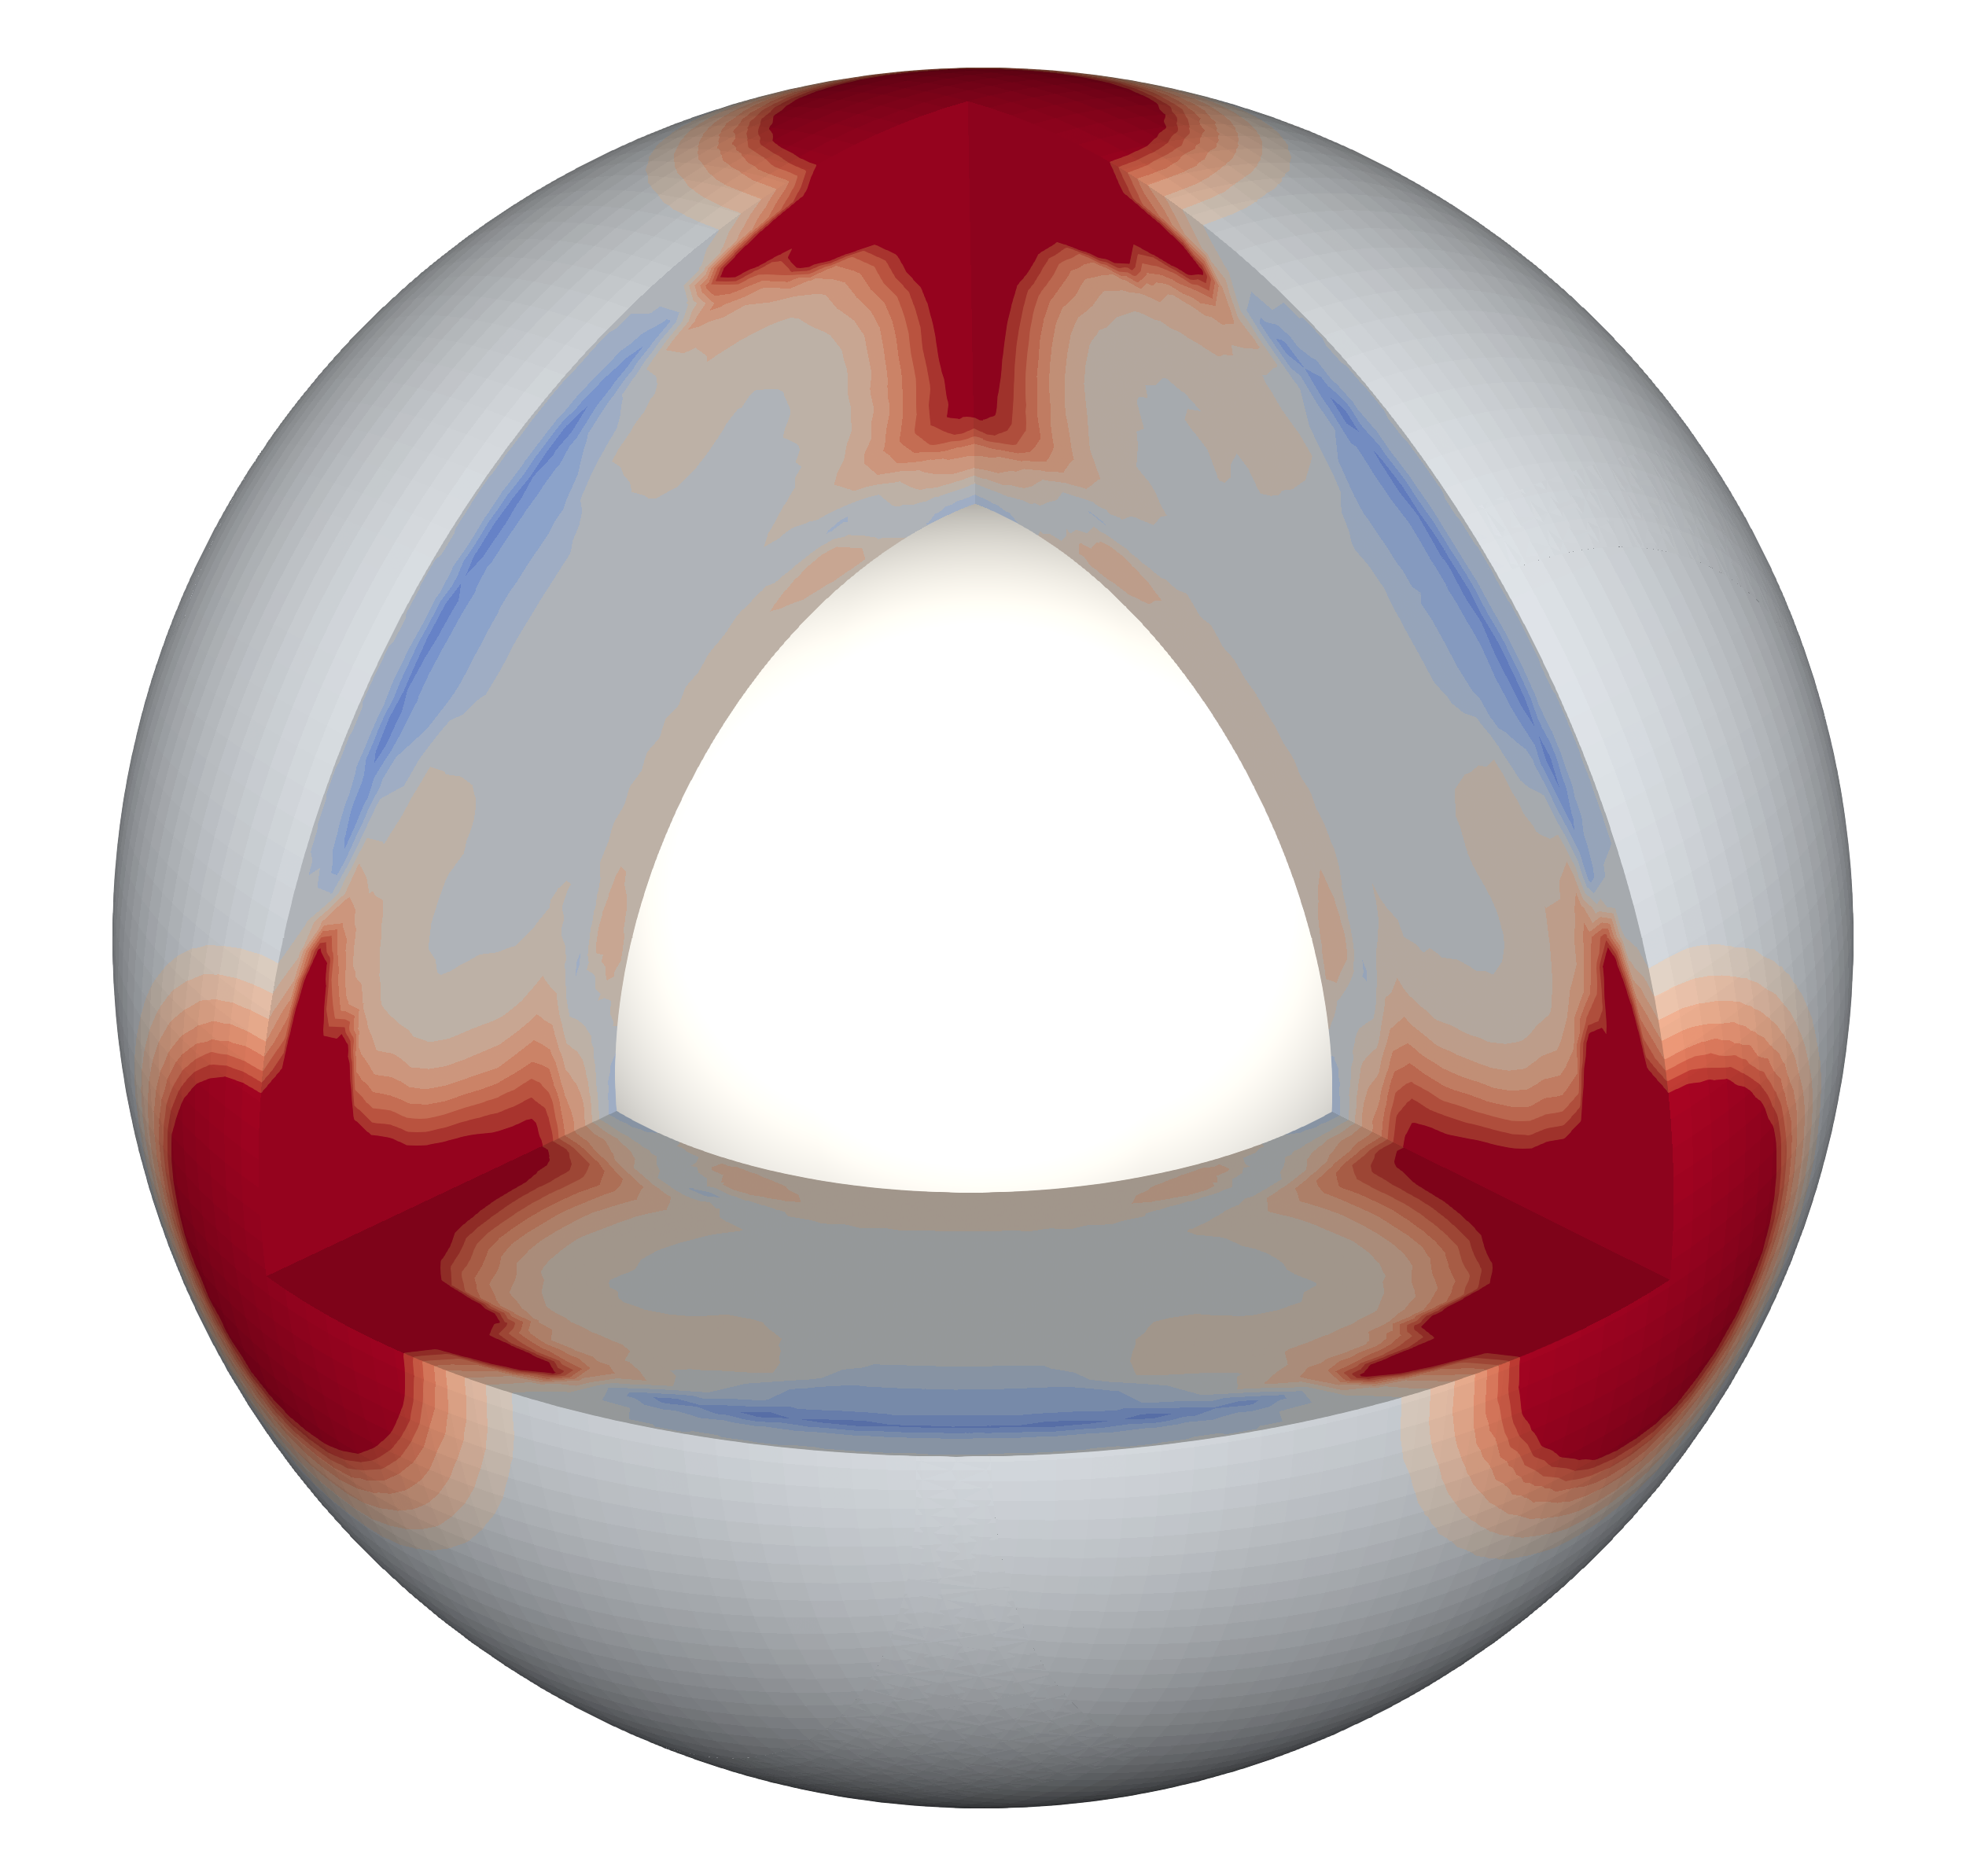
\includegraphics[width=12cm]{title/3Dspherical_global19.png}
\vspace{0.5cm}


 {\large \typeofthesis}\\[0.5cm]
{\large \today}\\[1cm] % Date, change the \today to a set date if you want to be precise
%----------------------------------------------------------------------------------------
%	AUTHOR SECTION
%----------------------------------------------------------------------------------------

\begin{flushleft}
\authorname\\% Your name
\end{flushleft}

\noindent\rule{16cm}{1pt}\\
\vspace{0.5cm}
%% Choose one of the following -- a colour or black-and-white logo
$\vcenter{\hbox{
\includegraphics[width=2.5cm]{title/LOGO-ERC.jpg}}}$
\hfill
$\vcenter{\hbox{
\includegraphics[width=8cm]{title/LOGO-NEWTON.png}}}$
\hfill
$\vcenter{\hbox{
\includegraphics[width=2.5cm]{title/LOGO-UNIPD.png}}}$\\

%\ifdefined\department
%\Large \department\\% Minor heading such as course title
%\fi
%\Large \school\\[1.5cm] % Minor heading such as course title
%----------------------------------------------------------------------------------------
%	DATE SECTION
%----------------------------------------------------------------------------------------


% 
\includegraphics[width=5cm]{title/LOGO-ERC.jpg}\\[1cm] 

%\vspace{1cm}
%
\includegraphics[width=4.cm]{title/LOGO-UNIPD.png}

\vfill % Fill the rest of the page with whitespace

\end{titlepage}
\pagenumbering{roman}

\newpage
\onehalfspacing%\raggedright %\raggedright turns off justification and hypenation

\tableofcontents
%\listoffigures
%\listoftables
\newpage
\section*{\Huge{Font styles}}
Throughout the manual, we have done our best to use different font styles indicating:
\begin{itemize}
    \item text
    \item \textbf{SOFTWARE} 
    \item \texttt{files, folders, URL links, commands}
    \item \fonts{variables present within the codes}
    \item \textbf{scalar, vectors, $2^{nd}$ and $4^{th}$ order tensors}
\end{itemize}

\newpage

\section*{\Huge{Nomenclature}}
Here we provide explanations for the different symbols, acronyms and variables found in this guide.

\begin{table}[ht!]
\small
\begin{tabular}{lp{11cm}l}
\\
\hline
Abbreviation&Description&Units\\
\hline
UM&Upper mantle\\
MTZ&Mantle Transition zone\\
UTZ&Upper Transition zone\\
LTZ&Lower Transition zone\\
LM&Lower Mantle\\
LPO&Lattice Preferred Orientation\\
SPO&Shape Preferred Orientation\\
\\
fse\textsubscript{max},fse\textsubscript{min}&maximum, minimum semiaxis of the FSE&$1$\\
ln\textsubscript{fse},ln\textsubscript{fse NODE}&natural logarithm of the ratio between the major and minor semiaxes of the FSE computed for an aggregate or a node of the Eulerian grid&$1$\\
$Vp_{max},Vp_{min}$&maximum, minimum P-wave velocity&$m/s$\\
$Vp_{anis}$&P-wave anisotropy&$\%$\\
$Vs_{1},Vs_2$&fast and slow S-wave components after splitting&$m/s$\\
$dVs_{MAX}$&maximum velocity difference between the fast and slow S-wave components&$\%$\\
$V_{SH},V_{SV}$&azimuthally averaged velocity of the S-wave polarized in the horizontal and vertical planes&$m/s$\\
$\xi$&radial anisotropy&1,$\%$\\
$G$&azimuthal anisotropy&1,$\%$\\
$\psi$&porosity&$1$\\
\\
P&Pressure &$Pa$\\
Tk&Temperature &$K$\\
Fd&Fraction of dislocation creep deformation &$1$\\
\textbf{V},V\textsubscript{i}&Velocity vector and its components&$m/s$\\
\textbf{D},D\textsubscript{ij}&$2^{nd}$ order velocity gradient tensor and its components&$s^{-1}$\\
\textbf{F},F\textsubscript{ij}&$2^{nd}$ order deformation gradient tensor and its components&$1$\\
\textbf{FSE} &$2^{nd}$ order left stretch tensor, whose eigenvalues and eigenvectors describe the Finite Strain Ellipsoid &$1$\\
\textbf{C},C\textsubscript{$\alpha\beta$}&$4^{th}$ order elastic tensor and its components in Voigt notation&$GPa$\\
%C\textsubscript{$\alpha\beta$}&Components of the $2^{nd}$ order elastic tensor in Voigt notation&$GPa$\\
\pmb{$\eta$},$\eta_{\alpha\beta}$&$4^{th}$ order normalized viscous tensor and its components in Voigt notation&$1$\\
%$\eta_{\alpha\beta}$&Components of the $2^{nd}$ order normalized viscous tensor in Voigt notation&$1$\\
\\
\hline
\end{tabular}
\end{table}

%\vspace{0.5cm}

The units on the rightmost column define variables when dimensional.

\mainmatter
\chapter{Introduction}
\label{chapter:introduction}

\section{General information about \thesistitle}

\thesistitle{} is a software package for modelling strain-/stress-induced rock fabrics and testing the effects of the resulting elastic and viscous anisotropy on seismic imaging and mantle convection patterns. 

\thesistitle{} includes programs for geodynamic modelling (\textbf{ECOMAN-geodynamics}) and seismological modelling (\textbf{ECOMAN-seismology}) that are mostly written in Fortran and Julia language, and where most of the routines are parallelized with a hybrid MPI and OpenMP scheme, providing strong scalability with increasing number of cores.

\textbf{ECOMAN-geodynamics} includes software for (Fig. \ref{fig:flowchart}):
\begin{enumerate}
\item Rock fabrics and mechanical properties simulations:

\begin{itemize}
    \item \textbf{\drexstitle}: Single Aggregate Fabric. This program builds on the original D-REX and estimates the strain-induced LPO of a single mantle aggregate. It includes the necessary \textbf{MTEX Toolbox} libraries to generate pole figures of the (1) LPO and (2) isotropic/anisotropic elastic properties.

    \item \textbf{\drexmtitle}: Multiple Aggregates Fabric. This program builds on the original D-REX and computes the strain-induced LPO of multiple mantle aggregates and output their (1) deformation gradient tensor \textbf{F} and (2) elastic tensor \textbf{C} as a function of the crystals orientation, volume fraction and of the local P-T conditions. 

    \item \textbf{\exevtitle}: this program computes the EXtrinsic Elastic and Viscous anisotropy using Effective Medium Theories (STILWE \citep{backus1962jgr} and DEM (e.g., \citep{mainprice1997tect})). It includes a parametrization of the viscous tensor evolution as a function of the deformation for 2 phases (matrix-inclusion) systems to be used in large-scale mantle convection simulations \citep{demontserrat2021}.


%\item \texttt{Draw.io} -- an online drawing package that can output PDFs to Google Drive -- see \url{https://www.draw.io}.
\end{itemize}

\item Visualisation of the mechanical properties and data formatting in preparation for seismological synthetics:

\begin{itemize}
    \item \textbf{\viztomotitle}: this program processes the \drexmtitle{} output for (1) visualization of the aggregates elastic and deformational history (FSE) properties, and (2) preparing the initial setup for seismic wave propagation simulations (e.g., \textbf{SPECFEM3D},\psitomotitle).
    
    \item \vizvisctitle: this program processes the \drexmtitle{} output for visualization of the aggregates viscous anisotropy and deformational history (FSE) properties.
\end{itemize}

\end{enumerate}

\textbf{ECOMAN-seismology} includes software for seismic forward and inverse modelling:
\begin{itemize}
    \item \textbf{\skstitle}: this program estimates the SKS splitting at a grid of virtual seismic stations placed at the top of the \drexmtitle{} model as a function of the back-azimuth using \textbf{FSTRACK} \citep{becker2006epsl}.
    
    \item \textbf{\psitomotitle}: this software performs isotropic and anisotropic P- and S- wave travel-time + S-wave splitting intensity inversions on either synthetic elastic models computed with \drexmtitle{} and \viztomotitle{} or with real datasets, and utilizing the method of \citep{vanderbeek2021,vanderbeek2023}. Other inversion methods to be added soon!.
\end{itemize}


\begin{figure}
    \centering
    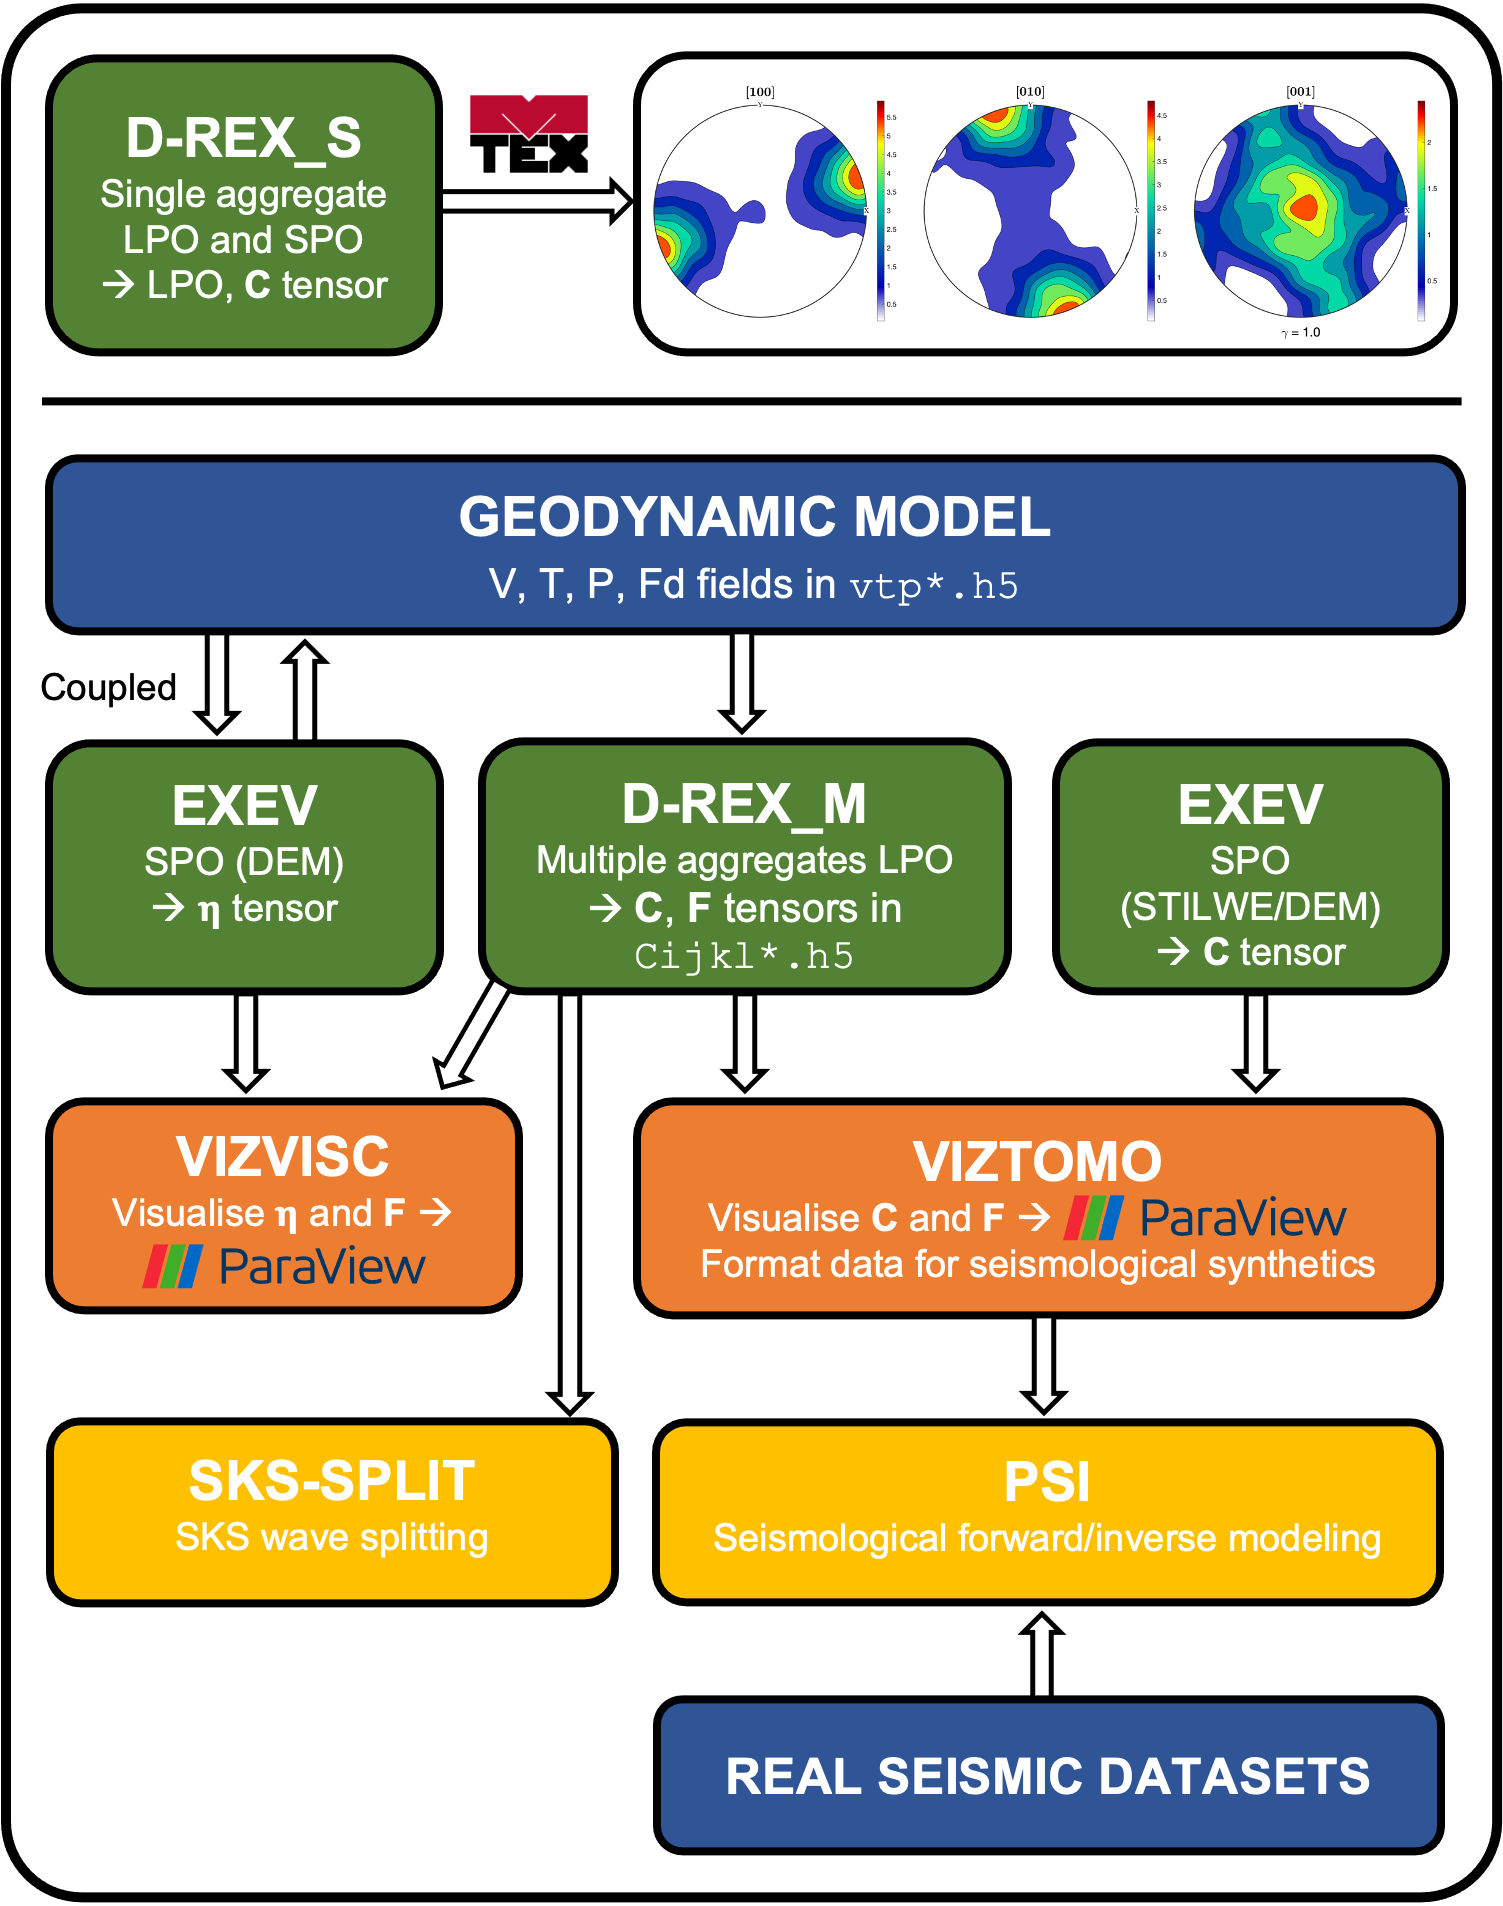
\includegraphics[width=1.0\textwidth]{introduction/FlowChartnew.png}
    \caption{\thesistitle{} structure and flow chart. Coloured boxes denote programs that compute rock fabrics (green), post-process the elastic (\textbf{C}), viscous ($\pmb{\eta}$) and deformation gradient (\textbf{F}) tensors for visualisation and/or data formatting for seismological synthetics (orange), perform seismological forward/inverse modelling on synthetic or real datasets (yellow).  Input data are from geodynamic modelling or real seismic datasets (blue). Visualisation of the mechanical properties and LPO can be done with the MTEX MATLAB toolbox for single crystal aggregates or the software Paraview for large-scale simulations.}
    \label{fig:flowchart}
\end{figure}

\section{Why \thesistitle?}
The understanding of the Earth’s interior is mainly based on seismological and geodynamic modelling, the first one providing important information about the present-day structure, while the second about the Earth’s geological history.
Seismological and geodynamical modelling are typically conducted separately, which creates difficulties in both interpreting seismic data in terms of geodynamic processes and in providing mantle structure constraints to geodynamic models.
From this perspective, \thesistitle{} aims at linking seismology and geodynamics by providing a set of software to estimate the mantle elastic properties as a function of the deformation history and local P-T conditions. The modelled elastic properties can be used to generate tomographic models and run forward/inverse seismological problems (as it is done with real datasets), and the output compared with observations. \\
In addition, \thesistitle{} allows estimating the role of extrinsic viscous anisotropy in large-scale mantle convection models by providing a parametrization of the strain-induced evolution of the SPO-related fabrics in two-phase (matrix-inclusions) systems.

When compared to other similar softwares/packages, \thesistitle:
\begin{itemize}
    \item aims at being a more versatile package suitable for any geodynamic simulations (2D/3D  cartesian/polar coordinate systems; regional/global settings),
    \item takes into account for the time-dependent deformational history of the mantle (which is usually not steady-state, especially close to plate boundaries),
    \item predicts the strain-induced fabric and elastic tensor of different mantle layers (i.e., not only the upper mantle),
    \item includes Effective Medium Theories (STILWE, DEM) and a parametrization of the fabric evolution of 2-phase composites to predict extrinsic elastic and viscous anisotropy, 
    \item generates realistic grid structures distributions of mantle elastic properties to be used for forward/inverse seismological modelling (e.g., \textbf{SPECFEM3D}, \psitomotitle).  
    \item performs synthetic seismic inversions (e.g., P- and S-wave travel-time tomographies, S-wave splitting intensities) within the computational domain, which facilitates the comparison with other tomographic models and the estimation of apparent anomalies (artefacts) due to, for example, unaccounted-for elastic anisotropy (\citep{bezada2016g3,vanderbeek2021,vanderbeek2023}) and/or regularisation. 


\end{itemize}

\section{Referencing and useful links}
If you use \thesistitle{}, please cite one of the following paper that best fits your application.

\begin{enumerate}
    \item New paper about \thesistitle{} (Faccenda et al., submitted)
    \item \citep{faccenda2013g3}: \drexmtitle{} methodology explained in detail; applied to upper mantle fabrics.
    \item \citep{faccenda2014pepi}: Extension of \drexmtitle{} to mantle fabrics of the MTZ and ULM; elastic tensors scaled by local P-T conditions.
    \item \citep{bezada2016g3}: First example of synthetic P-wave travel-time tomography on mantle fabrics generated with \drexmtitle.
    \item \citep{hu2017EPSL}: \drexmtitle{} goes spherical.
    \item \citep{faccenda2019JGR}: Evaluation of extrinsic elastic anisotropy in mantle aggregates.
    \item \citep{ferreira2019natgeo}, \citep{sturgeon2019g3}: Evaluation of lower mantle intrinsic and extrinsic fabrics to explain the observed seismic anisotropy.
    \item \citep{vanderbeek2021,vanderbeek2023}: Isotropic and anisotropic tomography with \psitomotitle{} on mantle fabrics generated with \drexmtitle.
    \item \citep{demontserrat2021}: submitted, viscous anisotropy due to extrinsic fabrics.
\end{enumerate}

\vspace{0.5cm}
Useful references and links:\\*

\textbf{\thesistitle{}} download: \url{https://github.com/ecoman-geos} \\* 

\textbf{\thesistitle{}} website: \url{https://newtonproject.geoscienze.unipd.it/ecoman/} \\*

\textbf{D-REX}: \url{http://www.ipgp.fr/~kaminski/} \citep{kaminski2004gji}\\*

\textbf{FSTRACK}: \url{https://github.com/thwbecker/fstrack} \citep{becker2006epsl}\\*

\textbf{MTEX Toolbox}: \url{https://mtex-toolbox.github.io/index.html} \citep{mainprice2011gsl}\\*

\textbf{\mmaeostitle{}}: \url{https://bitbucket.org/chust/eos} \citep{chust2017jgr}

\section{Author contribution}
\thesistitle{} was developed by Manuele Faccenda (geodynamic modelling and visualization), Brandon P. VanderBeek (developer of \psitomotitle{} module and of body-wave anisotropic inversion method), with fundamental contributions by Albert de Montserrat (derived and tested the parametrization of the extrinsic viscous anisotropy) and Jianfeng Yang (testing and applications). 

\section{Acknowledgements}
The development of \thesistitle{} has been funded by the ERC StG 758199 NEWTON and the Università di Padova FACCPRAT12 granted to Manuele Faccenda.
\chapter{Installation and compilation}
\label{chapter:installation}

Software included in the \thesistitle{} package run with the following compilers, libraries and software (see Table \ref{table:compile}):

\begin{itemize}
    \item Intel Fortran90 compiler
    \item Intel OpenMP, MPI compiler
    \item HDF5
    \item \paraviewtitle{} (version  5.4 or higher; \url{https://www.paraview.org/download/})
    \item \matlabtitle{} (version  R2018b or higher)
    \item \juliatitle{} (tested version 1.7.x - 1.9.x)
\end{itemize}

\vspace{1cm}

\begin{table}[h!]
\centering
\caption{\raggedright Required compilers and software for execution and visualization}
\begin{adjustbox}{width=1\textwidth}
\begin{tabular}{|m{0.30\textwidth}|m{0.38\textwidth}|m{0.32\textwidth}|} 

\hline
\textbf{Software}	& \textbf{Compilers/Libraries/Software}	& \textbf{Visualization Software} \\ [1ex] 
\hline\hline

\drexstitle{} & Intel F90, HDF5 & \matlabtitle{} (MTEX toolbox, version 5.* or higher) \\[1ex]\hline

\drexmtitle{} & Intel F90/OpenMP/MPI, HDF5 & - \\[1ex]\hline
 
\viztomotitle{}/\vizvisctitle & Intel F90/OpenMP, HDF5 & \paraviewtitle \\[1ex]\hline

\exevtitle{} & Intel F90/OpenMP, HDF5 & \matlabtitle\\[1ex]\hline

\skstitle{} & Intel F90, HDF5 & \matlabtitle{}, \paraviewtitle \\[1ex]\hline

\psitomotitle{} & \juliatitle{} & \paraviewtitle{} \\[1ex]\hline

\hline

\end{tabular}

\end{adjustbox}

%\raggedright \footnotesize{$^1$ In \drexstitle, \textbf{ptmod} is set in the input file.}\\

\label{table:compile}

\end{table}

\section{Installation}

1) Clone the source code(s): \\

\href{https://github.com/ecoman-geos/ECOMAN2.0-geodynamics.git}{\drexstitle{}, \drexmtitle{}, \exevtitle{}, \viztomotitle{}, \vizvisctitle}: \\
\texttt{git clone https://github.com/ecoman-geos/ECOMAN2.0-geodynamics.git}\\*

\href{https://github.com/ecoman-geos/ECOMAN2.0-seismology.SKS-SPLIT.git}{\skstitle{}}: \\
\texttt{git clone https://github.com/ecoman-geos/ECOMAN2.0-seismology.SKS-SPLIT.git}\\*

\href{https://github.com/ecoman-geos/ECOMAN2.0-seismology.PSI_D}{\psitomotitle{}}: \\
\texttt{git clone https://github.com/ecoman-geos/ECOMAN2.0-seismology.PSI\_D.git}\\*

2) To compile the F90 files, execute the \texttt{bash\_compile} file present in each software directory as \texttt{./bash\_compile}. The scripts should be compiled with the command \texttt{h5pfc} when the parallel HDF5 libraries are installed, or \texttt{h5fc} otherwise.\\

3) To run the F90 executables, see files RUN or pbs\_*

\section{Software dependencies}
\drexmtitle{} requires velocity field(s) and time constraints from a geodynamic model. To scale the elastic tensors by the local (P,T) conditions, pressure and temperature fields need to be additionally provided. Velocity, pressure and temperature field(s) and time are stored in \texttt{vtp*.h5} files.  \\
Software \viztomotitle{}, \vizvisctitle, \skstitle{} and \psitomotitle{} require the pre-computation of an elastic and/or deformation history model, and thus should be run after the execution of \drexmtitle{} (see Fig. \ref{fig:flowchart}). However, \psitomotitle{} can also be used with real seismic datasets\\
\vizvisctitle{} needs also the pre-computation of a database of viscous tensors through software \textbf{DEMviscous} included in directory \texttt{EXEV}.\\*


\chapter{\drexstitle: single mantle aggregate LPO fabrics with D-Rex}
\label{chapter:drexs}

\drexstitle{} is a software that is designed for testing the evolution of mantle fabrics and related elastic properties of a single aggregate, as a function of the flow field, amount of strain, crystal plasticity, P-T conditions and SPO fabrics. It builds on the original \textbf{D-Rex} software \citep{kaminski2004gji}.\\
Five different types of 2-phases mantle aggregates, hereafter named rocktypes, are available:\\ 
\vspace{0.1cm}


\fonts{1} = Ol:Ens, for the upper mantle (UM: 0-410 km)\\ 
\fonts{2} = Wd:Grt, for the upper transition zone (UTZ: 410-520 km)\\ 
\fonts{3} = Rw:Grt, for the lower transition zone (LTZ: 520-660 km)\\ 
\fonts{4} = Brd:MgO, for the lower mantle (LM: 660-2900 km)\\ 
\fonts{5} = pPv:MgO, for the bottom of the lower mantle\\ 

The LPO evolution is computed for Olivine, Enstatite, Wadsleyite, Bridgmanite and post-Perovskite, while other major phases such as Garnet, Ringwoodite and MgO are considered to be isotropic and their distribution is set to random.
Thus, no LPO is computed for rocktype \fonts{3}, and anisotropy in the LTZ arises only when SPO modeling is active.\\

The fabrics generated with \drexstitle{} can also be used to impose pre-existing microstructures on multiple crystal aggregates lying within a specific subdomain of large scale geodynamic models. The computed final LPO and F\textsubscript{ij} are saved to \texttt{fossilfabric.h5}, and can be subsequently loaded during the \drexmtitle{} simulations upon setting \fonts{fossilfabric} > 0 in \texttt{drexm\_input.dat} (see section \ref{section:modelsetup}).
\vspace{0.5cm}

\texttt{COMPILE: ./bash\_compile}\\*

\texttt{RUN: ./drexs drexs\_input.dat}\\*


\section{Parameter input file}

The following information need to be set in the parameter input file \texttt{drexs\_input.dat} (unless otherwise specified, the variable format is FORTRAN \texttt{double precision}):

A) Output file/directory name
\begin{itemize}
    \item \fonts{output\_name}: (String) if not existing, a new directory is created with output files saved each $0.1$ strain increment. The output files are named as\\ \texttt{[\fonts{output\_name}]+[strain]+[.h5]} (example: if \fonts{output\_name} = \texttt{UM\_},\\ \fonts{strain\_max} = 1.0, the output files will be \texttt{UM\_0.1.h5}, \texttt{UM\_0.2.h5}, \ldots, \texttt{UM\_1.0.h5}). When \fonts{spomod} > 0, an additional output file is generated at the end of the run named as \texttt{[\fonts{output\_name}]+[SPO.h5]} (example: \texttt{UM\_SPO.h5}).
\end{itemize}
\vspace{0.5cm}

B) Maximum strain
\begin{itemize}
    \item \fonts{strain\_max}
\end{itemize}
\vspace{0.5cm}

C) Velocity gradient tensor D\textsubscript{ij}
\begin{itemize}
    \item \fonts{D\textsubscript{11},...,D\textsubscript{32}}: components of the velocity gradient tensor
    
\end{itemize}
\vspace{0.5cm}

D) LPO parameters:
\begin{itemize}
    \item \fonts{size3}: (Integer) cubic root of total number of grains in the aggregate for each of the 2 mineral phases (e.g.: \fonts{size3} = 10 $\rightarrow$ 1000 crystals of phase 1 and 1000 crystals of phase 2). 
    \item \fonts{rocktype}: (Integer) define the mantle aggregate (\fonts{1},\fonts{2},\fonts{3},\fonts{4},\fonts{5})
\end{itemize}
\vspace{0.5cm}

\hspace{0.5cm} For each of the 5 different types of aggregate\footnotemark:
\vspace{0.5cm}

\footnotetext{Rw and Grt are assumed to be isotropic at MTZ depths, and therefore no LPO is computed for this aggregate. Consequently, only \fonts{Xol} and \fonts{single\_crystal\_elastic\_db} need to be set.}

\begin{itemize}
    \item \fonts{Xol}: volume fraction of Ol, Wd, Rw, Brd, pPv (in \%)
    \item \fonts{stressexp}: stress exponent for non-Newtonian plasticity  
    \item \fonts{Mob}: efficiency of grain boundary migration 
    \item \fonts{chi ($\pmb{\chi}$)}: volume fraction threshold below which no dislocation creep occurs   :e
    \item \fonts{lambda ($\pmb{\lambda}$)}: efficiency of grain nucleation
    \item \fonts{fractdislrock}: fraction of deformation accommodated by the anisotropic phase
    \item \fonts{tau1...tauN}: normalized CRSS of the anisotropic phase slip systems. For upper mantle aggregates (rocktype = 1), tau(1,1-4) are for olivine, while tau(1,5)=1 is for enstatite. See \ref{table:1}.
    \item \fonts{single\_crystal\_elastic\_db}: (Integer) choose single crystal elastic tensor for phase 1 and 2 from those compiled in elastic\_database.f90. See \ref{table:2}.
\end{itemize}

\vspace{1cm}

E) Operating modes:
\begin{itemize}

    \item \fonts{ptmod}: (Integer)
    \begin{itemize}
        \item[] \fonts{0} = use single crystal tensors at room P-T conditions
        \item[] \fonts{1} = scale elastic moduli by local P-T conditions defined below
    \end{itemize}
    \item \fonts{eosmod}:  (Integer) set the domain lithology (\fonts{1}: Dunite; \fonts{2}: Harzburgite; \fonts{3}: Pyrolite; \fonts{4}: Basalt; \fonts{5}: Pyroxenite) for which the corresponding lookup tables of density, isotropic Vp and Vs computed with \mmaeostitle{} are loaded (see Table \ref{table:3}). The isotropic Vp and Vs are used to compute the isotropic component of the elastic tensor scaled at the local P-T conditions.
    \item \fonts{pressure}: pressure (in GPa)
    \item \fonts{tkelv}: temperature (in Kelvin)
    \item \fonts{fractvoigt}: fraction of Voigt averaging scheme when calculating the aggregate elastic tensor in \%. It varies from 0.0 (Reuss average) to 100.0 (Voigt average). When equal to 50.0, it yields the Hill average.
    
    \item \fonts{spomod}:  (Integer) when > 0, computes extrinsic elastic anisotropy\footnotemark{} saved in output file \texttt{[\fonts{output\_name}]+[SPO.h5]}
    \begin{itemize}
        \item[] \fonts{0} = no extrinsic elastic anisotropy
        \item[] \fonts{1} = extrinsic elastic anisotropy due to grain-scale or rock-scale layering (STILWE model)
        \item[] \fonts{2} = extrinsic elastic anisotropy due to the presence of aligned inclusions (DEM model)
        \item[] \fonts{3} = extrinsic elastic anisotropy due to the presence of aligned inclusions (DEM model) superimposed over the LPO fabric.
    \end{itemize}
\end{itemize}

\footnotetext{The SPO modeling is explained in detail in section \textbf{\ref{section:elasticSPO}}}

\section{Fabric visualization}
Fabric visualization requires the installation of the \texttt{MTEX toolbox} (\citet{mainprice2011gsl}). A recently tested version is 5.10.2, but previous versions 5.* should work as well. Please refer to the MTEX download webpage (\url{https://mtex-toolbox.github.io/download}) for installation instructions. 
\\
The aggregate fabric can be visualized with the \matlabtitle{} script \texttt{/viz/read\_Cij\_LPO.m} that allows to plot pole figures of the LPO, Vp, Vs1 and dVs, for multiple output files, which then can be combined into animations, together with the possibility to display the evolving fabric strength (M-index, J-index), anisotropy and its components (obtained with tensor decomposition; \citet{browaeys2004gji}) as a function of strain.
\\
The control parameters to be set in the first part of the script are (Fig. \ref{fig:drexs_viz}, Fig. \ref{fig:atype}, Fig. \ref{fig:miji}, Fig. \ref{fig:azirad}, Fig. \ref{fig:dec}):
\begin{itemize}
    \item \fonts{input\_dir}: (String) path to \drexstitle{} output files directory.
    \item \fonts{output\_dir}: (String) output directory where images and videos are saved.
    \item \fonts{fname0}: (String) first part of output file name (same as \fonts{output\_name} in \texttt{drexs\_input.dat}).
    \item \fonts{min\_strain}, \fonts{stp\_strain}, \fonts{max\_strain}: minimum, increment and maximum strain as indicated in the second part of the output file name to be visualized. When \fonts{min\_strain} = \fonts{max\_strain}, only a single output file is visualized.
    \item \fonts{plot\_Cij\_LPO}:  (Boolean) when true, activates plotting pole figures for Vp, dVs and LPOs. 
    
    \begin{itemize}
        \item \fonts{plot\_Voigt}:  (Boolean) when true, plot Vp, Vs1, dVs due to aggregate LPO, Voigt average.
        \item \fonts{plot\_Reuss}:  (Boolean) when true, plot Vp, Vs1, dVs due to aggregate LPO, Reuss average.
        \item \fonts{plot\_Mixed}:  (Boolean) when true, plot Vp, Vs1, dVs due to aggregate LPO, mixed Voigt/Reuss average as specified by \fonts{fractvoigt} in \texttt{drexs\_input.dat}.
        \item \fonts{plot\_Phase1LPO}: (Boolean) when true, plot LPO pole figures of main anisotropic phase, together with a plot of the M-index and J-index.
        \item \fonts{plot\_Phase2LPO}: (Boolean) when true, plot LPO pole figures of enstatite, together with a plot of the M-index and J-index (only for UM aggregates).
    \end{itemize} 
    
    \item \fonts{makevideo}: (Boolean) when true, generate animations of Vp, dVs and LPO pole figures evolution as specified by the 5 \fonts{plot\_*} operational modes defined above. 
    
    \item \fonts{plot\_azirad}: (Boolean) when true, plot azimuthal and radial P and S anisotropy, and $\eta$ parameter, as a function of strain for the tensors activated with \fonts{plot\_Voigt}, \fonts{plot\_Reuss}, \fonts{plot\_Mixed}.

    \item \fonts{plot\_dec}: (Boolean) when true, plot (i) the norm of the total anisotropy component of the tensor over the norm of the full tensor (in \%), and (ii) the norm of each anisotropic component of the tensor normalized over the norm of the total anisotropic component (in \%). These have been obtained by decomposition (\citet{browaeys2004gji} of the elastic tensor (Mixed average) and saved in file \texttt{anisdec.h5]}.
    
    \item \fonts{plot\_SPO}: (Boolean) when true, plot Vp, dVs due to SPO from the \texttt{[\fonts{output\_name}] +[SPO.h5]} output file.  
        
    \item \fonts{printmod}: (Boolean) when true, save images in \texttt{*.png} format.
\end{itemize}
\vspace{1.0cm}

\begin{figure}[ht]
    \centering
    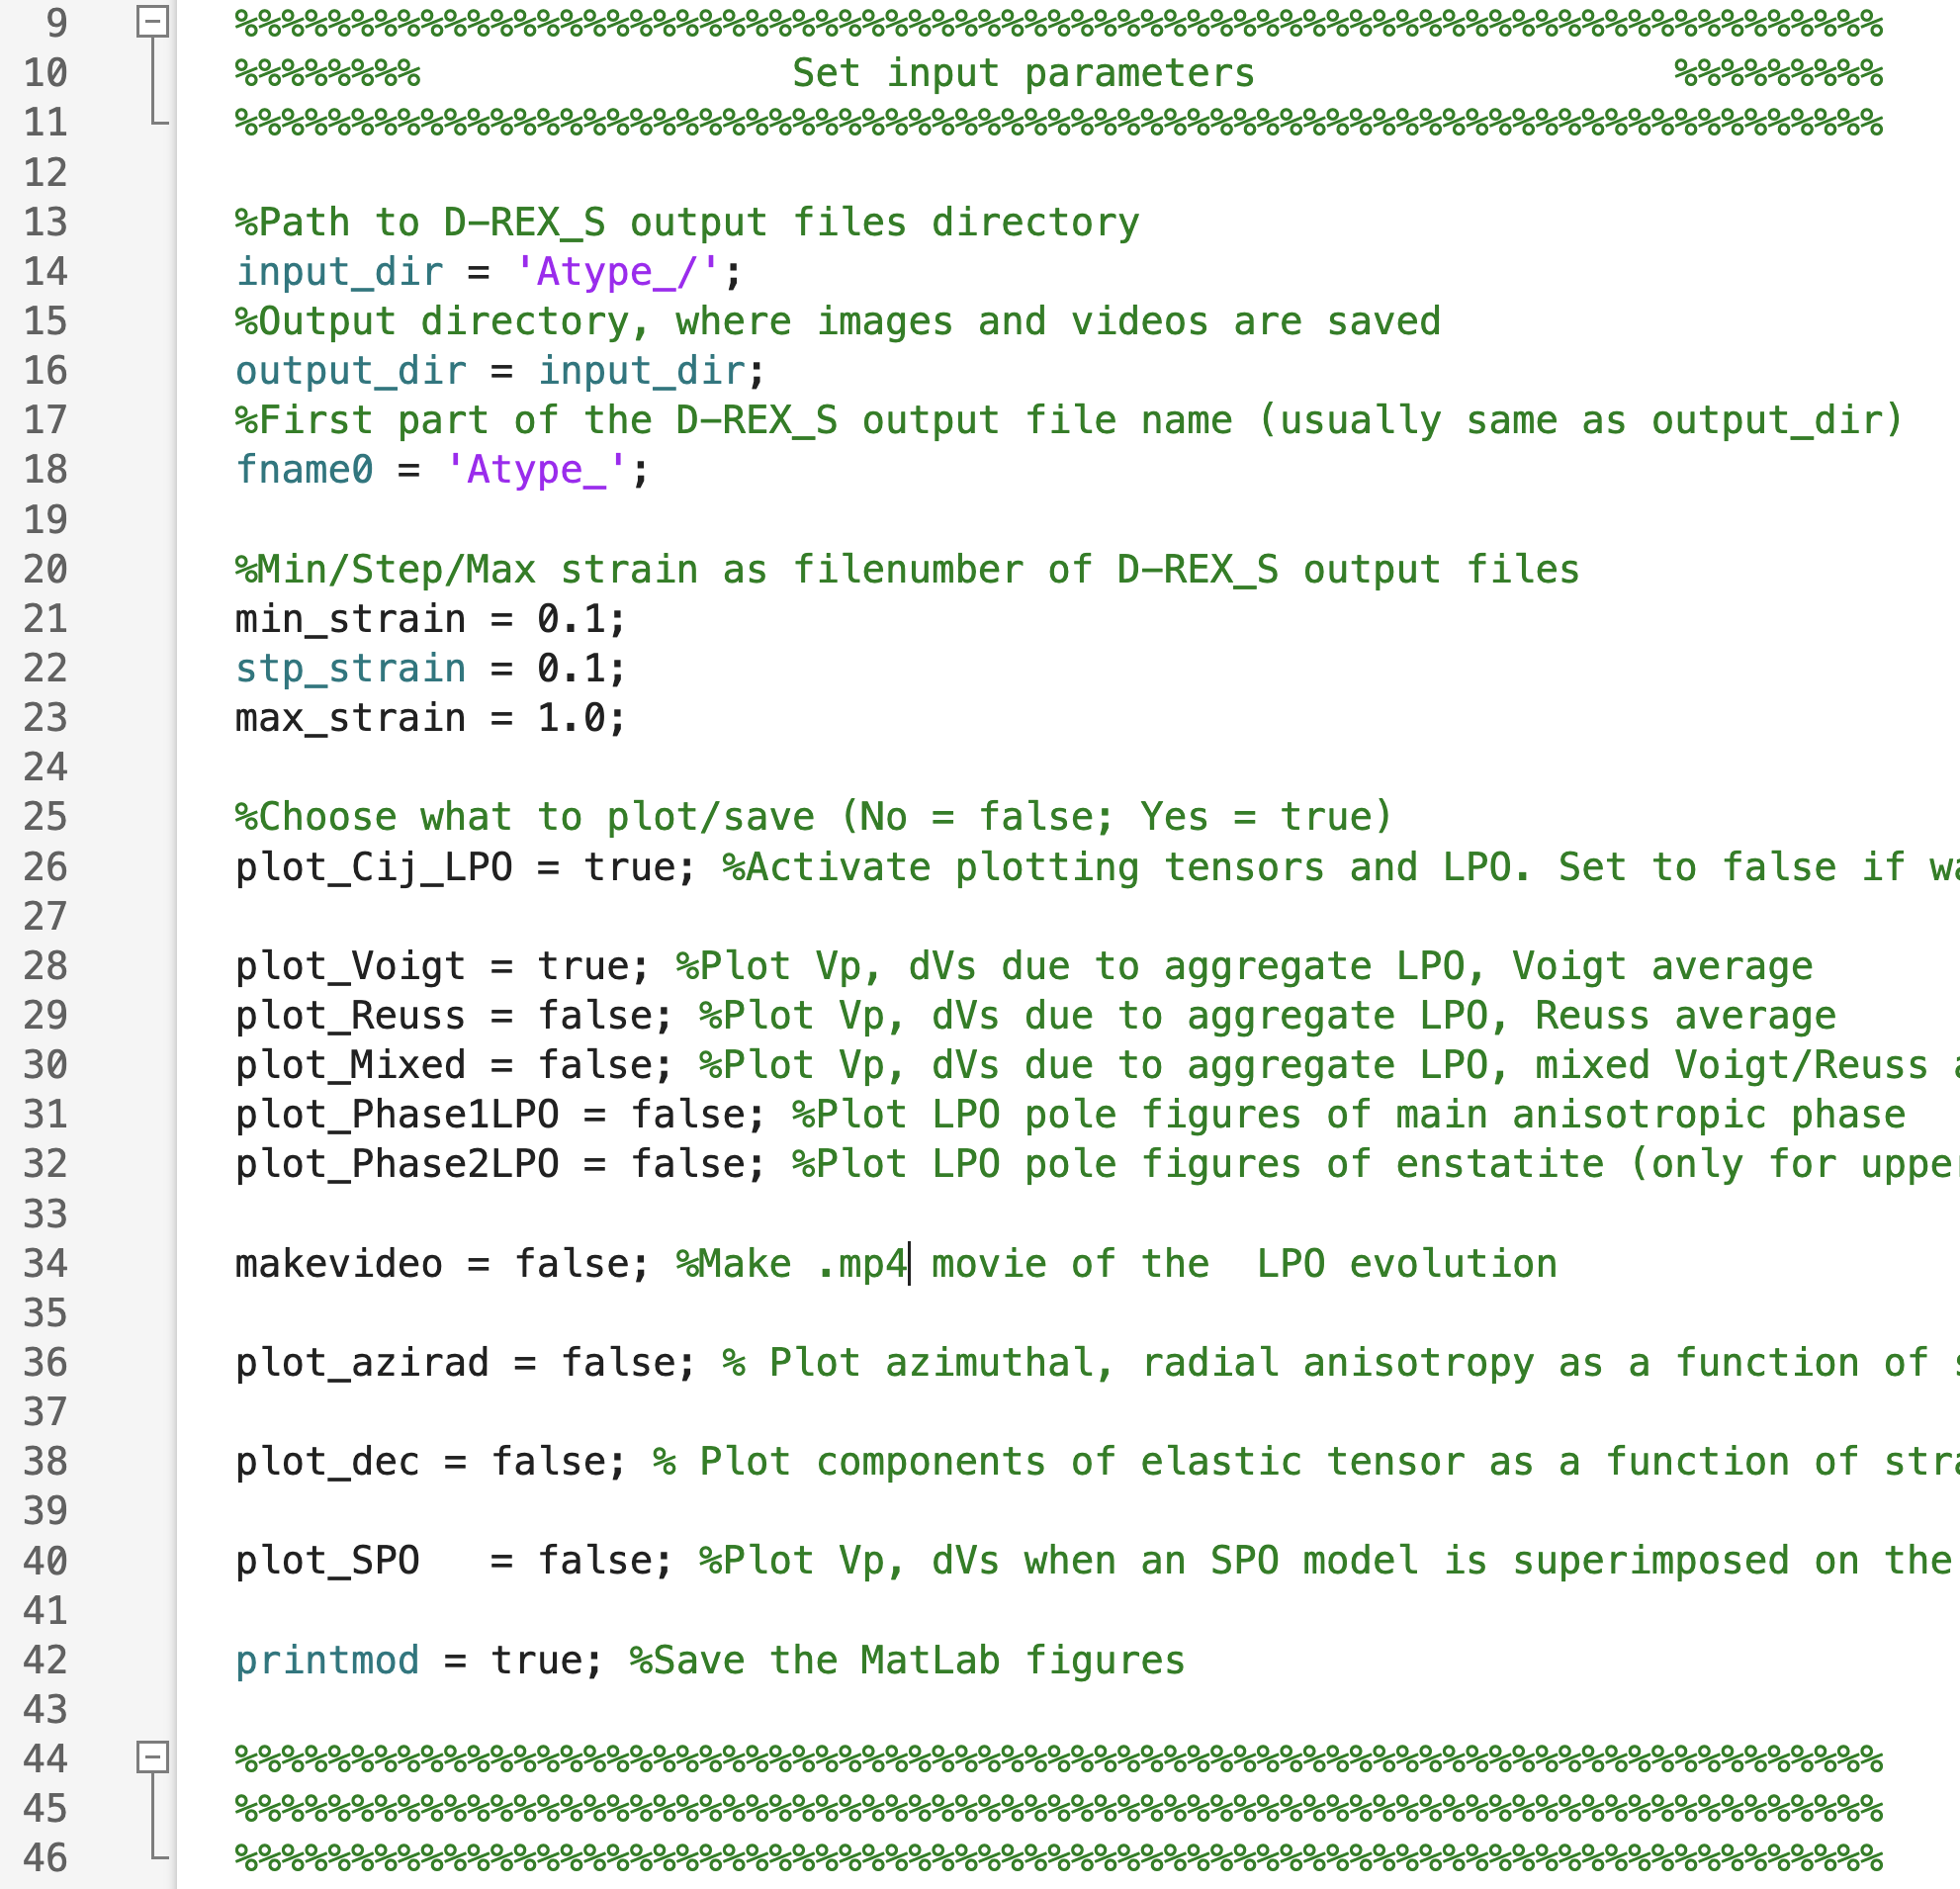
\includegraphics[width=1.0\textwidth]{DREX_S/drexs_viz.png}
    \caption{Control parameters in \texttt{read\_Cij\_LPO.m} for visualizing the \drexstitle{} output. In this particular case: generate pole figures of Vp, Vs1 and dVs for the elastic tensor obtained with the Voigt averaging scheme.}
    \label{fig:drexs_viz}
\end{figure}

\begin{figure}[ht]
    \centering
    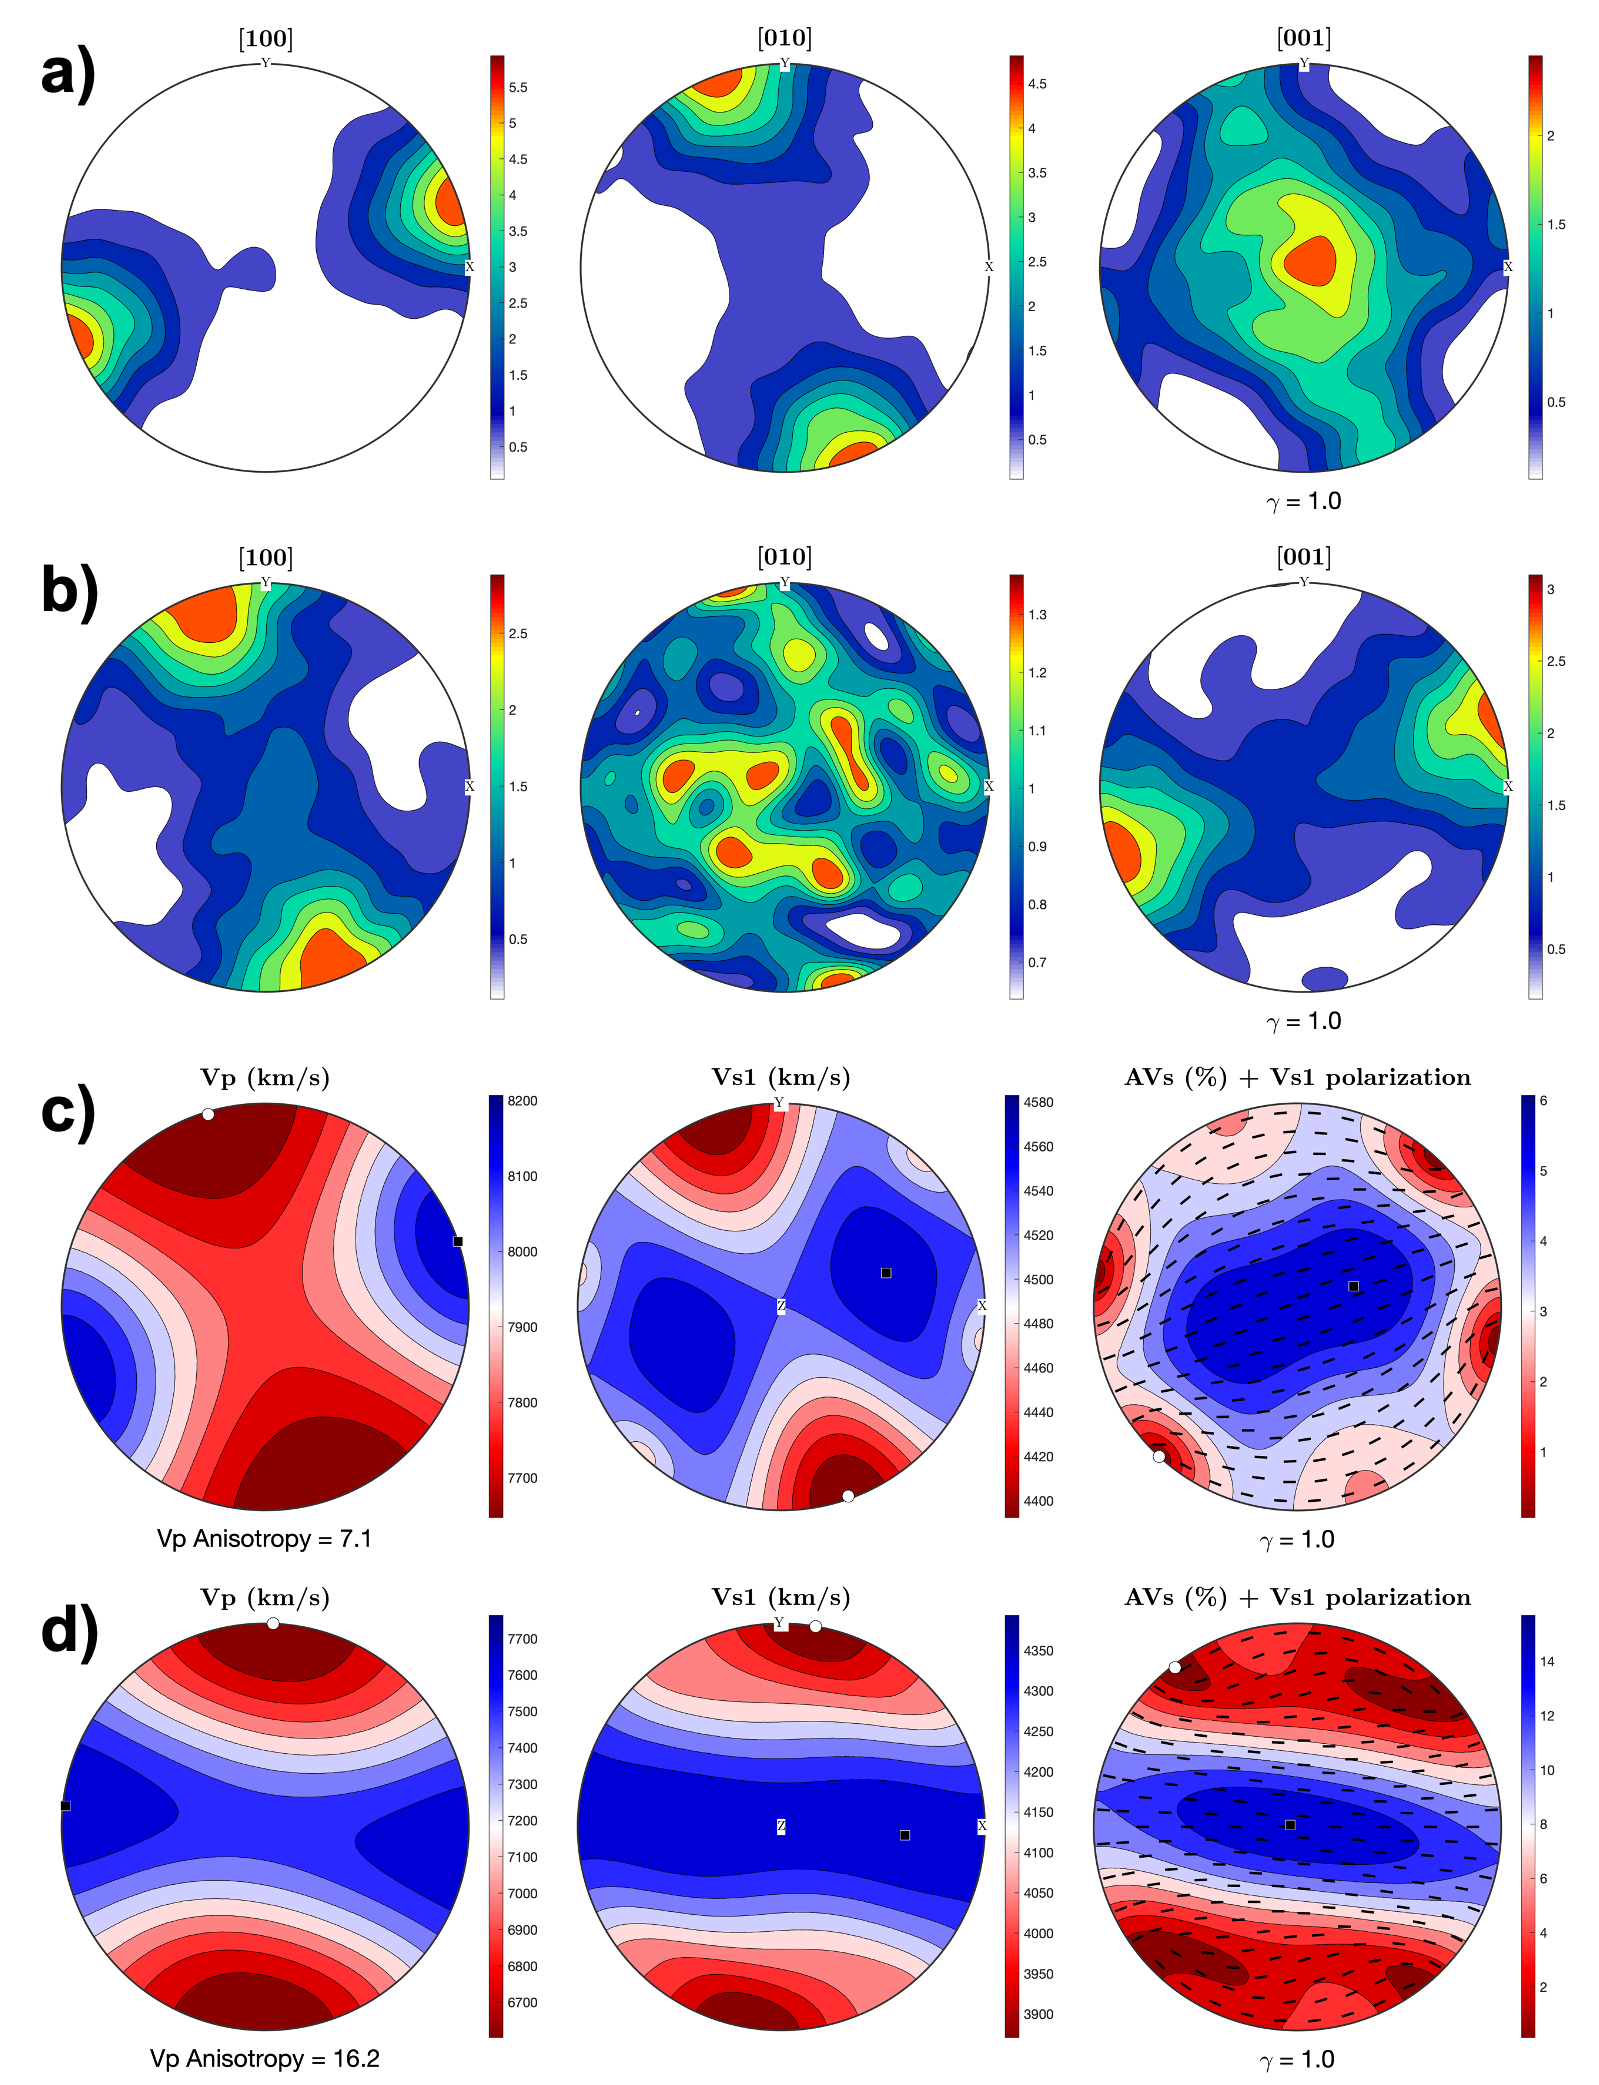
\includegraphics[width=1.0\textwidth]{DREX_S/Atype_summary_manual.png}
    \caption{Example of UM fabric after right-lateral simple shear strain of 1.0 with Ol:Ens = 70:30, \fonts{Mob} = 10, $\pmb{\lambda}=5$, $\pmb{\chi}=0.3$. (A) Olivine (A-type) LPO; (B) Enstatite LPO; (C) Vp, Vs1, and dVs + polarization direction of the fast shear wave component for the Mixed (Hill average) elastic tensor  resulting from the LPO fabrics in (A) and (B); (D) same as (C) but with superimposed an SPO fabric due to 5\% of melt-filled inclusions (10:10:1) oriented at -30$^{\circ}$ from the principal stress axis (which is at 45$^{\circ}$ from the horizontal plane).}
    \label{fig:atype}
\end{figure}

\begin{figure}[ht]
    \centering
    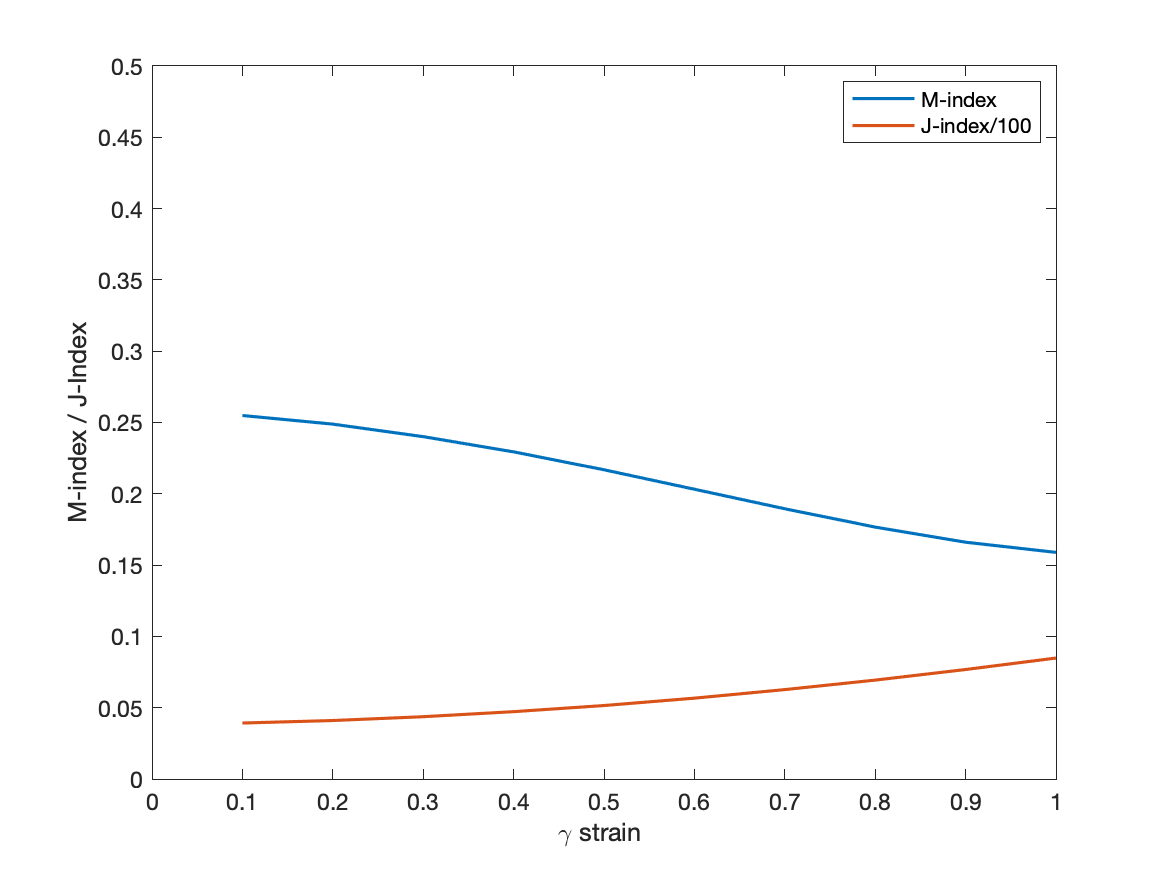
\includegraphics[width=1.0\textwidth]{DREX_S/MI_JI_Atype_.png}
    \caption{Evolution of M-index and J-index for an A-type olivine fabric.}
    \label{fig:miji}
\end{figure}

\begin{figure}[ht]
    \centering
    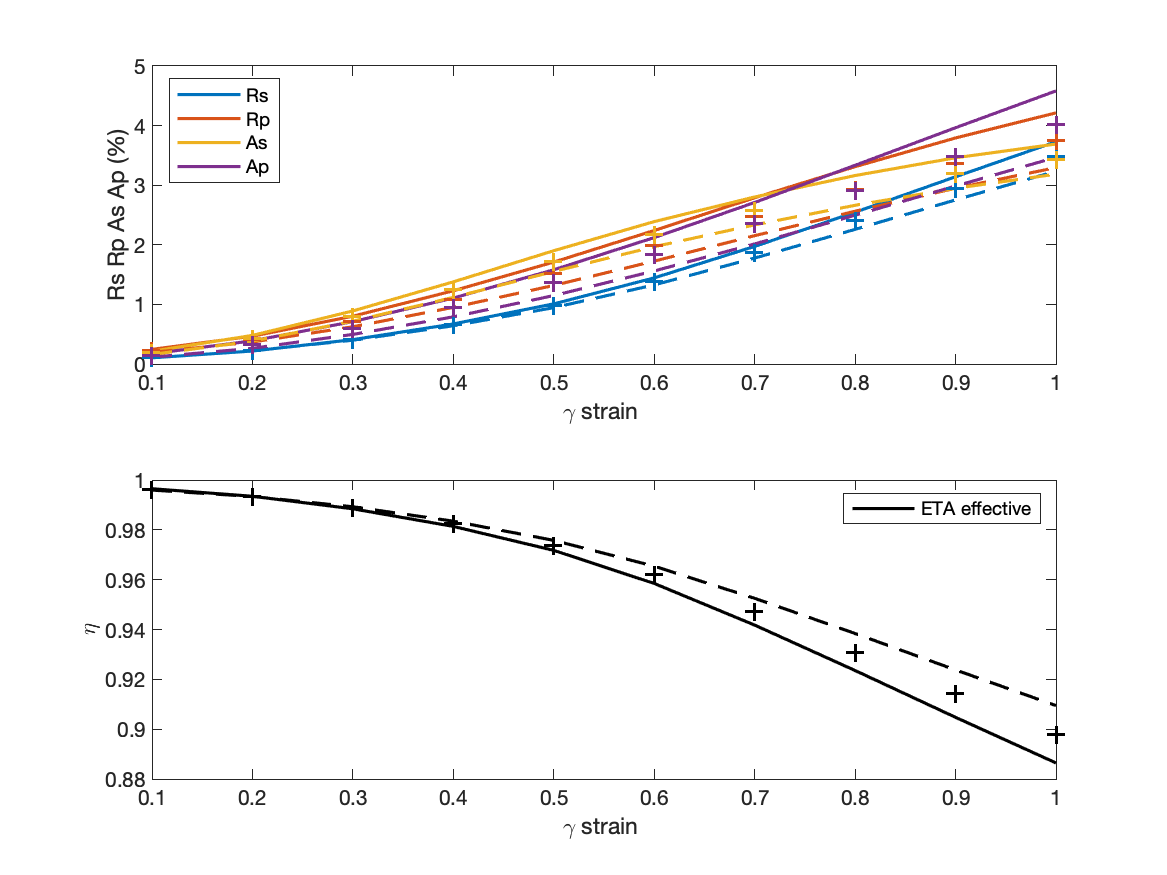
\includegraphics[width=1.0\textwidth]{DREX_S/AziRad.png}
    \caption{Evolution of radial and azimuthal P and S-wave anisotropy, and $\eta$ parameter for Voigt (continuous lines), Reuss (dashed lines) and Hill (+ symbols) averages.}
    \label{fig:azirad}
\end{figure}

\begin{figure}[ht]
    \centering
    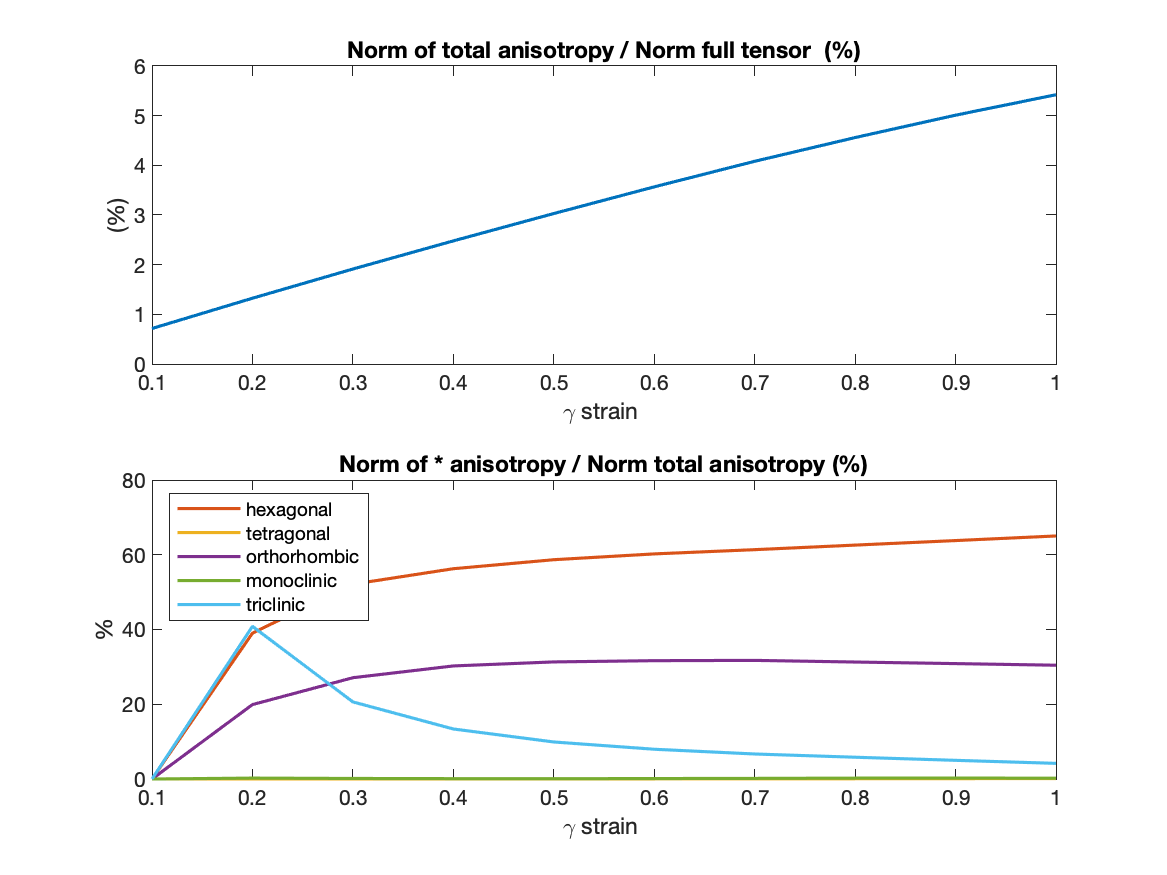
\includegraphics[width=1.0\textwidth]{DREX_S/dec.png}
    \caption{Evolution of (top) the norm of the total anisotropy component of the tensor over the norm of the full tensor (in \%), and (bottom) the norm of each anisotropic component of the tensor normalized over the norm of the total anisotropic component (in \%), computed for the elastic tensor obtained with the Mixed average.}
    \label{fig:dec}
\end{figure}

\vfill % Fill the rest of the page with whitespace
\chapter{\drexmtitle: multiple mantle aggregates LPO fabrics with D-Rex}
\label{chapter:drexm}

\drexmtitle{} is a software that computes the evolution of the LPO and related elastic properties of multiple mantle aggregates, as a function of the flow field, deformation mechanisms and P-T conditions given by large-scale geodynamic simulations, and of the single crystal plastic and elastic properties. It builds on the original \textbf{D-Rex} software \citep{kaminski2004gji}.\\
\\
The original \textbf{D-Rex} code estimates the strain-induced LPO of upper mantle polycrystalline aggregates in 2D assuming steady-state flow and that the whole deformation is accommodated by dislocation creep \citep{kaminski2004gji}.\\*
\drexmtitle{} additionally accounts for:
\begin{itemize}
    \item non steady-state flows in 2D/3D cartesian/polar grids \citep{faccenda2013g3,hu2017EPSL}. The fabrics for global-scale simulations are computed using the Yin-Yang grids (\citet{kageyama2004g3});
    
    \item fabrics within the mid and lowermost mantle, including those for post-Perovskite. Phase transitions can be set to occur at defined depths (e.g., 410 km, 660 km), density crossovers (which allows modeling the deflection of phase boundaries with a non-null Clapeyron-slope), and parameterized phase boundary as for the case of Brd -> pPv \citep{oganov2004nature};  
    
    \item elastic properties scaled by local P-T conditions \citep{faccenda2014pepi,chang2016natcomm,ferreira2019natgeo}. The isotropic component of the elastic tensors is taken from the lookup tables generated with \mmaeostitle{} for different lithologies, while the anisotropic component from the pressure and temperature derivatives of the single crystal elastic moduli. This strategy ensures a gradual transition of the elastic properties at phase boundaries where mineral aggregate transformation occurs;
    
    \item fabric evolution in presence of multiple creep mechanisms. Only the fraction of deformation accommodated by dislocation creep is used for intracrystalline deformation, while the remaining for rigid body rotation (e.g., \citep{hedjazian2017EPSL});
    
    \item imposing a pre-existing (fossil) fabric (pre-computed with \drexstitle{}) within a subdomain, typically the lithosphere. This is often the case for geodynamic models where the lithosphere accretion is not modeled, and its geometry is initially prescribed;
    
    \item extrinsic elastic anisotropy \citep{faccenda2014pepi,sturgeon2019g3} which can be superimposed over the LPO fabrics during visualization of the output with \viztomotitle{} (see section \textbf{\ref{section:elasticSPO}}).
    
    \item parallelization of its routines using a hybrid MPI and OpenMP scheme.

\end{itemize}
\vspace{0.5cm}
\texttt{COMPILE: ./bash\_compile}\\*

\texttt{RUN: mpirun -np nprocs ./drexm drexm\_input.dat}\\*

\section{Software structure and modus operandi}
\drexmtitle{} is structured as the following:
\begin{enumerate}
    \item the \drexmtitle{} model parameters are loaded from \texttt{drexm\_input.dat}, and the Eulerian grid (where the Eulerian fields are defined) and Lagrangian grid (mantle aggregates distribution) initialized accordingly. 
    \item the \textbf{V} (velocity), \textbf{P} (pressure), \textbf{Tk} (temperature), \textbf{Fd} (fraction of deformation accommodated by dislocation creep) Eulerian fields of the geodynamic model are loaded from the input \vtptitle{} files. 
    \item firstly, the mantle aggregates are advected backward in time for a desired time span (note that is different from the original D-Rex where the particles are advected backward in time for a desired amount of strain).
    \item successively, the mantle aggregates are advected forward and the strain-induced LPO and F\textsubscript{ij} evolution are simultaneously calculated. The forward run status can be checked in \texttt{cycle.txt} displaying the processed \vtptitle{} file number and the terminated iterations/cycles.  
    \item output \cijkltitle{} files are generated containing, among other infos, the elastic tensor \textbf{C}, density and the deformation gradient tensor \textbf{F} of each aggregate. 
\end{enumerate}

\section{Coordinate systems}
The coordinate system of the \drexmtitle{} computational domain is defined by axis 1, axis 2 and, in 3D, axis 3.\\
In cartesian coordinates, axis 1 is the horizontal direction, axis 2 depth, and, in 3D, axis 3 is the second horizontal direction.\\
In polar coordinates, axis 1 is longitude (in degrees), axis 2 the radial distance, and in 3D, axis 3 is colatitude (in degrees).\\
The vertical axis 2 can be positive either upward or downward.

\section{Input \vtptitle{} files}
In order to perform the operations mentioned in the previous section, input files named \vtptitle{}, where * is the file number, must be provided containing information about the geodynamic model evolution.

Essential information the input \vtptitle{} files should contain is:
\begin{itemize}
    \item the total elapsed time \fonts{timesum} and the timestep \fonts{dt} (time interval over which the fields are representative; normally it is the difference with the total elapsed time of the previous input \vtptitle{} file, if any. See section \ref{section:often}) of the geodynamic model as a HDF5 attribute \texttt{/Time}.
    \item the components of the Eulerian velocity vector field \textbf{V} saved in \texttt{/Nodes/V1}, \texttt{/Nodes/V2}, and in 3D, \texttt{/Nodes/V3}.
\end{itemize}

In addition, the following Eulerian fields can be provided:
\begin{itemize}
    \item when the geodynamic model is thermo-mechanical, the temperature \textbf{Tk} and total pressure \textbf{P} fields saved in \texttt{/Nodes/Tk} and \texttt{/Nodes/P}. These fields will be used to compute the elastic tensors as a function of the local P-T conditions.
    \item when the rheological model is based on multiple visco-plastic deformation mechanisms, the fraction of deformation accommodated by dislocation creep saved in \texttt{/Nodes/Fd}, where \textbf{Fd} = $nu_{disl}/nu_{eff}$, 0 $\leq$ \textbf{Fd} $\leq$ 1, $nu_{disl}$ is the viscosity calculated with the dislocation creep flow law, $nu_{eff}$ is the effective viscosity which is typically calculated with the harmonic average of each of the viscosities representing a different deformation mechanism. 
\end{itemize}

Summarizing, the time infos and the velocity field are essential, while the other 3 fields are optional and depend on the type of (mechanical vs. thermomechanical) geodynamic and (single vs. multiple visco-plastic deformation mechanisms) rheological models.

\subsection{How saving information from your geodynamic model?}
Examples of how to build the input file in HDF5 format with \matlabtitle{} are provided in directory \texttt{/D-REX\_M/make\_HDF5\_vtp\_files}.

\textbf{Indexing}: since the \textbf{V}, \textbf{P}, \textbf{Tk}, \textbf{Fd} Eulerian fields are loaded as 1D HDF5 datasets, they must be provided as 1D arrays where the nodes are indexed going through the grid axes sequenced as:
2D models: axis 2, axis 1. That is, Y, X axes in cartesian coordinates, and Radial, Long. axes in polar coordinates.
3D models: axis 2, axis 1, axis 3. That is, Y, X, Z axes in cartesian coordinates, and  Radial, Long., Colat. axes in spherical coordinates. 

\textbf{Units}: values in attribute \texttt{/Time} and \textbf{V} as well as those of variables (i.e., \fonts{timemax} or distances) in the input file \texttt{drexm\_input.dat} should be provided using consistent units for time and length, and which can be of any type (e.g., dimensional (i.e., [cm,yr] or [m,s]) or adimensional). In contrast, the \textbf{P} and \textbf{Tk} Eulerian fields must always be in Pa and K.

The Eulerian fields of the geodynamic model must be defined on the same node positions of the Eulerian grid defined in \texttt{drexm\_input.dat}. The Eulerian grid must be regular (i.e., same node spacing along a given axis; if other types of grid are required, please contact the software developer).\\
For 3D global-scale simulations, the Yin-Yang Eulerian grids \citep{kageyama2004g3} are used to ensure a more homogeneous sampling of the spherical domain (see section \ref{section:cookbook_3Dspherical_global}).\\ 
In cartesian coordinates, the velocity field can also be defined on staggered additional nodes, which allows to compute the velocity gradient tensor with a numerical resolution that is double than when the velocity vector components are all defined on the same basic node.  
In 2D, V1 is shifted by $+\Delta x_2/2$ and V2 by $+\Delta x_1/2$ with respect to the basic node. 
In 3D, V1 is shifted by $+\Delta x_2/2$ and $+\Delta x_3/2$, V2 by $+\Delta x_1/2$ and $+\Delta x_3/2$, V3 by $+\Delta x_1/2$ and $+\Delta x_2/2$ with respect to the basic node.

\subsection{How often saving information from your geodynamic model?}
\label{section:often}
\textbf{Time-dependent flows}: From our experience, for Earth-like deformation rates it is sufficient to save the \textbf{V}, \textbf{P}, \textbf{Tk} and \textbf{Fd} fields averaged every 100/200 kyr, a time span over which these fields do not vary substantially. This will prevent outputting too many files from the geodynamic model. The code will then calculate an advection timestep which fulfill the Courant criterion and iterate for several cycles upon reaching the timestep defined in \texttt{/Time}.\\

\textbf{Steady-state flows}: in this case, it is clear that only a single \vtptitle{} file is needed.

\subsection{Which is the model time interval over which \drexmtitle{} should run?}
\citep{boneh2014epsl} showed that a cumulative strain of 5 is sufficient to reset any previous LPO and develop a new one. This is indeed the maximum cumulative strain that the original \textbf{D-Rex} consider for LPO calculation of each mantle aggregate.
For typical mantle deformation rates of $10^{-15}-10^{-14}    s^{-1}$, this amount of deformation is acquired in about  3 – 30 Myr. This is the model time interval during which input \vtptitle{} files must be saved in your time-dependent geodynamic model. Thus, saving an input \vtptitle{} file every 200 kyr over a time span of 20 Myr, implies saving and processing 100 input files.\\
There exist cases where the model time interval could be larger, such as when it is desired to model the fabrics forming at oceanic ridges and successively advected for several tens of Myr within the rigid lithosphere till the subduction zone. However, steady-state corner flow is often assumed for this particular set of models, which implies that only a single \vtptitle{} file is needed.

\section{Output \cijkltitle{} files}
Output files includes, for each aggregate, its rocktype, position, density, elastic tensor \textbf{C} and deformation gradient tensor \textbf{F}. When available, the aggregate P-T conditions are additionally saved.
The \textbf{C} tensor is calculated as a function of the crystals orientation, volume fraction, modal composition of the aggregate (e.g., 70:30=Ol:Ens in hartzburgitic mantle), single crystal elastic properties scaled by the local P-T conditions, and with a Reuss-Voigt averaging scheme.\\
An output \cijkltitle{} file is always generated at the end of the simulation, whereby the aggregates, after the backward and forward advection episodes, display the same initial (regular) distribution. Output files at intermediate steps can be generated by setting \fonts{OutputStep} smaller than the total number of computing cycles of the forward advection scheme, with the characteristic that the aggregate distribution will be irregular. 

\section{Allocated memory}
Memory is allocated in large part to track the mineral aggregates properties and, to a minor extent, for storing the loaded the Eulerian node fields. Thus in case of 100s of thousands or millions of aggregates, problems related to insufficient memory allocation may occur.\\
For a 3D model, the memory allocated for the Eulerian fields is up to $24*8$ bytes per node. Thus, around 200 MB of memory is necessary every 1 million nodes per each MPI process.\\
For each mineral aggregates, the allocated memory is up to $(75 + 20*\fonts{size3})*8$ bytes, thus very sensitive to the number of crystals. When $\fonts{size3}=8$, there are $512*2$ crystals per aggregate, and thus 82.5 kB per aggregate. Hence, over 80 GB of memory is necessary every 1 million aggregates.

\section{Parameter input file}
\label{section:modelsetup}

The following information need to be set in the parameter  input file \texttt{drexm\_input.dat} (unless otherwise specified, the variable format is \texttt{double precision}):

MPI proc distribution along axis
\begin{itemize}
    \item \fonts{nproc1}, \fonts{nproc2}, \fonts{nproc2}: (Integer) number of MPI subdomains (processes) along axes 1, 2 and 3
\end{itemize}
(WARNING: the number of MPI processes \fonts{nproc1}*\fonts{nproc2}*\fonts{nproc3} must be > 1)
\vspace{1cm}

A) Input and output directories/files
\begin{itemize}
    \item \fonts{input\_dir}: (String) path to the input \vtptitle{} files directory (the path should end with  “/” )
    \item \fonts{output\_dir}: (String) path to the directory where the output \cijkltitle{} file is saved (the path should end with  “/” )
    \item \fonts{Tinit, Tstep, Tend}: (Integers) initial, increment and final number of input \vtptitle{} files. Set \fonts{Tinit} = \fonts{Tend} for steady-state models. 
    \item \fonts{OutputStep}: (Integer) number of cycles interval after which an output file is generated during forward advection.
    \item \fonts{timemax}: time span (in Myr for dimensional time) for steady-state models
\end{itemize}
\vspace{1cm}

B) Define the computational domain:
\begin{itemize}
    \item \fonts{dimensions}: (Integer)
        \begin{itemize}
         \item[] \fonts{2} = 2D model
         \item[] \fonts{3} = 3D model
        \end{itemize}
    \item \fonts{cartspher}:  (Integer) 
        \begin{itemize}
         \item[] \fonts{1} = cartesian coordinate system
         \item[] \fonts{2} = polar coordinate system
        \end{itemize}
    \item \fonts{basicstag}: velocity field defined on:  (Integer) 
        \begin{itemize}
         \item[] \fonts{1} = basic nodes
         \item[] \fonts{2} = staggered nodes\footnotemark
    \end{itemize}
\end{itemize}

\vspace{0.2cm}

Eulerian grid (i.e., where the \textbf{V}, \textbf{P} and \textbf{Tk} fields are defined):
\begin{itemize}

    \item \fonts{x1min}, \fonts{x1max}, \fonts{nx1}, \fonts{x1periodic}: define Eulerian axis 1: min, max coordinates (in unit length in cartesian coord.; in degrees in polar/spherical coord.), number of nodes (Integer), periodic (\fonts{1}) or not (\fonts{0}) (Integer).  
    \item \fonts{x2min}, \fonts{x2max}, \fonts{nx2}, \fonts{x2periodic}: define Eulerian axis 2: min, max coordinates (in unit length), number of nodes (Integer), periodic (\fonts{1}) or not (\fonts{0}) (Integer).  
    \item \fonts{x3min}, \fonts{x3max}, \fonts{nx3}, \fonts{x3periodic}: define Eulerian axis 3: min, max coordinates (in unit length in cartesian coord.; in degrees in spherical coord.), number of nodes (Integer), periodic (\fonts{1}) or not (\fonts{0}) (Integer).  
\end{itemize}

\vspace{0.2cm}
Lagrangian grid (i.e., the initial and final position of the mantle aggregates):
 
\begin{itemize}   
    \item \fonts{mx1min}, \fonts{mx1max}, \fonts{mx1stp}: define particle distribution along axis 1: min, max coordinates (in unit length in cartesian coord.; in degrees in polar/spherical coord.), spacing (in unit length, also for polar coordinate system)
    \item \fonts{mx2min}, \fonts{mx2max}, \fonts{mx2stp}: define particle distribution along axis 2: min, max coordinates, spacing (in unit length)
    \item \fonts{mx3min}, \fonts{mx3max}, \fonts{mx3stp}: define particle distribution along axis3: min, max coordinates (in unit length in cartesian coord.; in degrees in spherical coord.), spacing (in unit length, also for polar coordinate system)
\end{itemize}
\vspace{1cm}

\footnotetext{The staggered nodes can be defined only for cartesian grids}


C) LPO parameters:
\begin{itemize}
    \item \fonts{size3}\footnotemark: (Integer) cubic root of total number of grains in the aggregate for each of the 2 mineral phases (e.g.: \fonts{size3} = 10 $\rightarrow$ 1000 crystals of phase 1 and 1000 crystals of phase 2). 
\end{itemize}
\vspace{0.5cm}

\footnotetext{The size of the allocated memory is mostly sensitive to this parameter, be careful!}

    For each of the 5 different rocktype (Ol:Ens; Wd:Grt; Rw:Grt\footnotemark; Brd:MgO; pPv:MgO\footnotemark):
\begin{itemize}
    \item \fonts{Xol}: volume fraction of Ol, Wd, Rw, Brd, pPv (in \%)
    \item \fonts{minx2,maxx2}: min, max vertical distribution (in unit length)
    \item \fonts{stressexp}: stress exponent for non-Newtonian plasticity  
    \item \fonts{Mob}: efficiency of grain boundary migration 
    \item \fonts{chi ($\pmb{\chi}$)}: volume fraction threshold below which no dislocation creep occurs   
    \item \fonts{lambda ($\pmb{\lambda}$)}: efficiency of grain nucleation
    \item \fonts{fractdislrock}: fraction of deformation accommodated by the anisotropic phase. It assumes values between 0.0 (no deformation) and 1.0 (all deformation accommodated by the anisotropic phase). It should be always 1.0 for UM aggregates where both olivine and enstatite are anisotropic.
    \item \fonts{tau1...tauN}: normalized CRSS of the anisotropic phase slip systems. For upper mantle aggregates, one additional tau5=1 is added for enstatite. See \ref{table:1}.
    \item \fonts{single\_crystal\_elastic\_db}: (Integer) choose single crystal elastic tensor for phase 1 and 2 from those compiled in \texttt{elastic\_database.f90}. See \ref{table:2}.
\end{itemize}

\footnotetext{Rw and Grt are considered as isotropic at MTZ, and therefore only \textbf{Xol,minx2,maxx2} and \textbf{single\_crystal\_elastic\_db} need to be set}
\footnotetext{the occurrence of pPv is set according to the parametrized phase boundary by \citet{oganovono2004nature}, and therefore \textbf{minx2,maxx2} should not be set. Hence, \fonts{ptmod} = 2}

\vspace{1cm}

D) Pre-existing (fossil) fabric. The fabric (given by the LPO and \textbf{F}) computed for a single aggregate in directory \texttt{/D-REX\_S} is assigned to all aggregates within a given subdomain defined below:
\begin{itemize}
    \item \fonts{fossilfabric}: (Integer)
    \begin{itemize}
        \item[] \fonts{0} = no pre-existing fabric 
        \item[] \fonts{1} = the pre-existing fabric is set after backward advection and before computing the LPOs 
        \item[] \fonts{2} = the pre-existing fabric is set at the end of the model replacing the computed LPOs
    \end{itemize}
    \item \fonts{mx1minfab}, \fonts{mx1maxfab}: distribution of aggregates with pre-existing fabric along axis 1 (in unit length in cartesian coord.; in degrees in polar/spherical coord.)
    \item \fonts{mx2minfab}, \fonts{mx2maxfab}: distribution of aggregates with pre-existing fabric along axis 2 (in unit length)
    \item \fonts{mx3minfab}, \fonts{mx3maxfab}: distribution of aggregates with pre-existing fabric along axis 3 (in unit length in cartesian coord.; in degrees in spherical coord.)
\end{itemize}
In polar coordinates, the loaded LPO and \textbf{F} are rotated according to the aggregate longitude and colatitude. Thus, when computing the single aggregate fabric with \texttt{/D-REX\_S}, bear in mind that axis 1, 2 and 3 should correspond to longitude, depth and colatitude, respectively. 
\vspace{1cm}

E) Operating modes:
\begin{itemize}

    \item \fonts{fsemod}: (Integer)
    \begin{itemize}
        \item[] \fonts{0} = compute strain-induced \textbf{F} and LPO evolution
        \item[] \fonts{1} = compute only \textbf{F} evolution, and \fonts{fractdislmod}, \fonts{fabrictransformmod} and \fonts{ptmod} are set to 0.
    \end{itemize}
    
    \item \fonts{uppermantlemod}: (Integer)
    \begin{itemize}
        \item[] \fonts{0} = \textbf{F}, LPO and advection for all aggregates.
        \item[] \fonts{1} = \textbf{F} and LPO only for upper mantle aggregates; advection for all aggregates. This mode is suggested when focusing on UM anisotropy only. The elastic tensor of deeper mantle aggregates are computed assuming isotropy. As a consequence, the execution of the run is much faster.
    \end{itemize}
    
    \item \fonts{fractdislmod}: (Integer)
    \begin{itemize}
        \item[] \fonts{0} = 100\% of the deformation is accommodated by dislocation creep. 
        \item[] \fonts{1} = use only fraction of deformation accommodated by dislocation creep as interpolated from the \textbf{Fd} field. The \textbf{Fd} field need to be provided in input \vtptitle{} files.
    \end{itemize}
    
    \item \fonts{fabrictransformod}: (Integer)
    \begin{itemize}
        \item[] \fonts{0} = no phase transformation.
        \item[] \fonts{1} = retain LPO after phase transformation, simulating axisymmetric topotactic growth of the new phases.
        \item[] \fonts{2} = reset LPO after phase transformation
    \end{itemize}
    
    \item \fonts{ptmod}: (Integer)
    \begin{itemize}
        \item[] \fonts{0} = use single crystal tensors at room P-T conditions. Choose this when your geodynamic model is purely mechanical and there no is information about the local P-T conditions.
        \item[] \fonts{1} = scale elastic moduli and density by local P-T conditions, phase transitions occur at depths specified in top and bot; thus, the phase boundaries are horizontal. \textbf{Tk} and \textbf{P} fields need to be provided in input \vtptitle{} files.
        \item[] \fonts{2} = scale elastic moduli and density by local P-T conditions, phase transitions occurs at density crossovers (Ol+Ens $\leftrightarrows$ Wd+Grt at  3650 \si{kg/m^3}; Wd+Grt $\leftrightarrows$ Rw+Grt at  3870 \si{kg/m^3}; Rw+Grt $\leftrightarrows$ Brd+MgO at  4150 \si{kg/m^3}). This mode allows to model deflections of phase boundaries in proximity of mantle downwellings/upwellings. \textbf{Tk} and \textbf{P} fields need to be provided in input \vtptitle{} files.
    \end{itemize}
    
    The occurrence of pPv is determined with the parametrized phase transition by \citet{oganov2004nature}, thus \textbf{Tk} and \textbf{P} fields are necessary. In general, whenever the computational domain includes layers deeper than the upper mantle, \fonts{ptmod} > 0 is the preferred operational mode.
    
    In order to minimize the contrast in elastic properties among rocktypes and arising from contrasts in experimental single crystal elastic tensors and their P-T derivatives (see \ref{table:2}), the isotropic component of the aggregate elastic tensor is replaced with that computed with \mmaeostitle{} for a given lithology when \fonts{ptmod} > 0.
    
    \item \fonts{eosmod}: (Integer) set the domain lithology (\fonts{1}: Dunite; \fonts{2}: Harzburgite; \fonts{3}: Pyrolite; \fonts{4}: Basalt; \fonts{5}: Pyroxenite) for which the corresponding density, Vp and Vs lookup tables computed with \mmaeostitle{} are loaded (see Table \ref{table:3}).
    
    \item \fonts{fractvoigt}: fraction of Voigt averaging scheme when calculating the aggregate elastic tensor in \%. It varies from 0.0 (Reuss average) to 100.0 (Voigt average). When equal to 50.0\%, it yields the Hill average.
    
\end{itemize}

\section{Parallelization and its efficiency}
\drexmtitle{} routines are parallelized using a hybrid MPI and OpenMP scheme to take advantage of multi-CPU nodes and multicore architectures of modern HPC clusters. The parallel efficiency is close to 1 for most routines, with the update of the LPO and Fij tensor during the forward advection is the most time-consuming part of the run (Fig. \ref{fig:scalability}). The small performance degradation is due to the initialization of the Eulerian/Lagrangian grids and arrays, and to I/O operations (i.e., loading infos from input \vtptitle{} files, writing the output to \cijkltitle{})\\ which are executed serially within each process. As a result, the efficiency of the time-dependent flow models (such as the 3D sinking slab model) is lower than that of steady-state models (the 3D global flow model) because of the larger I/O operations ((i.e., loading infos from input \vtptitle{} files and compute the velocity gradient tensors, advection timestep, etc.).

\begin{figure}
    \centering
    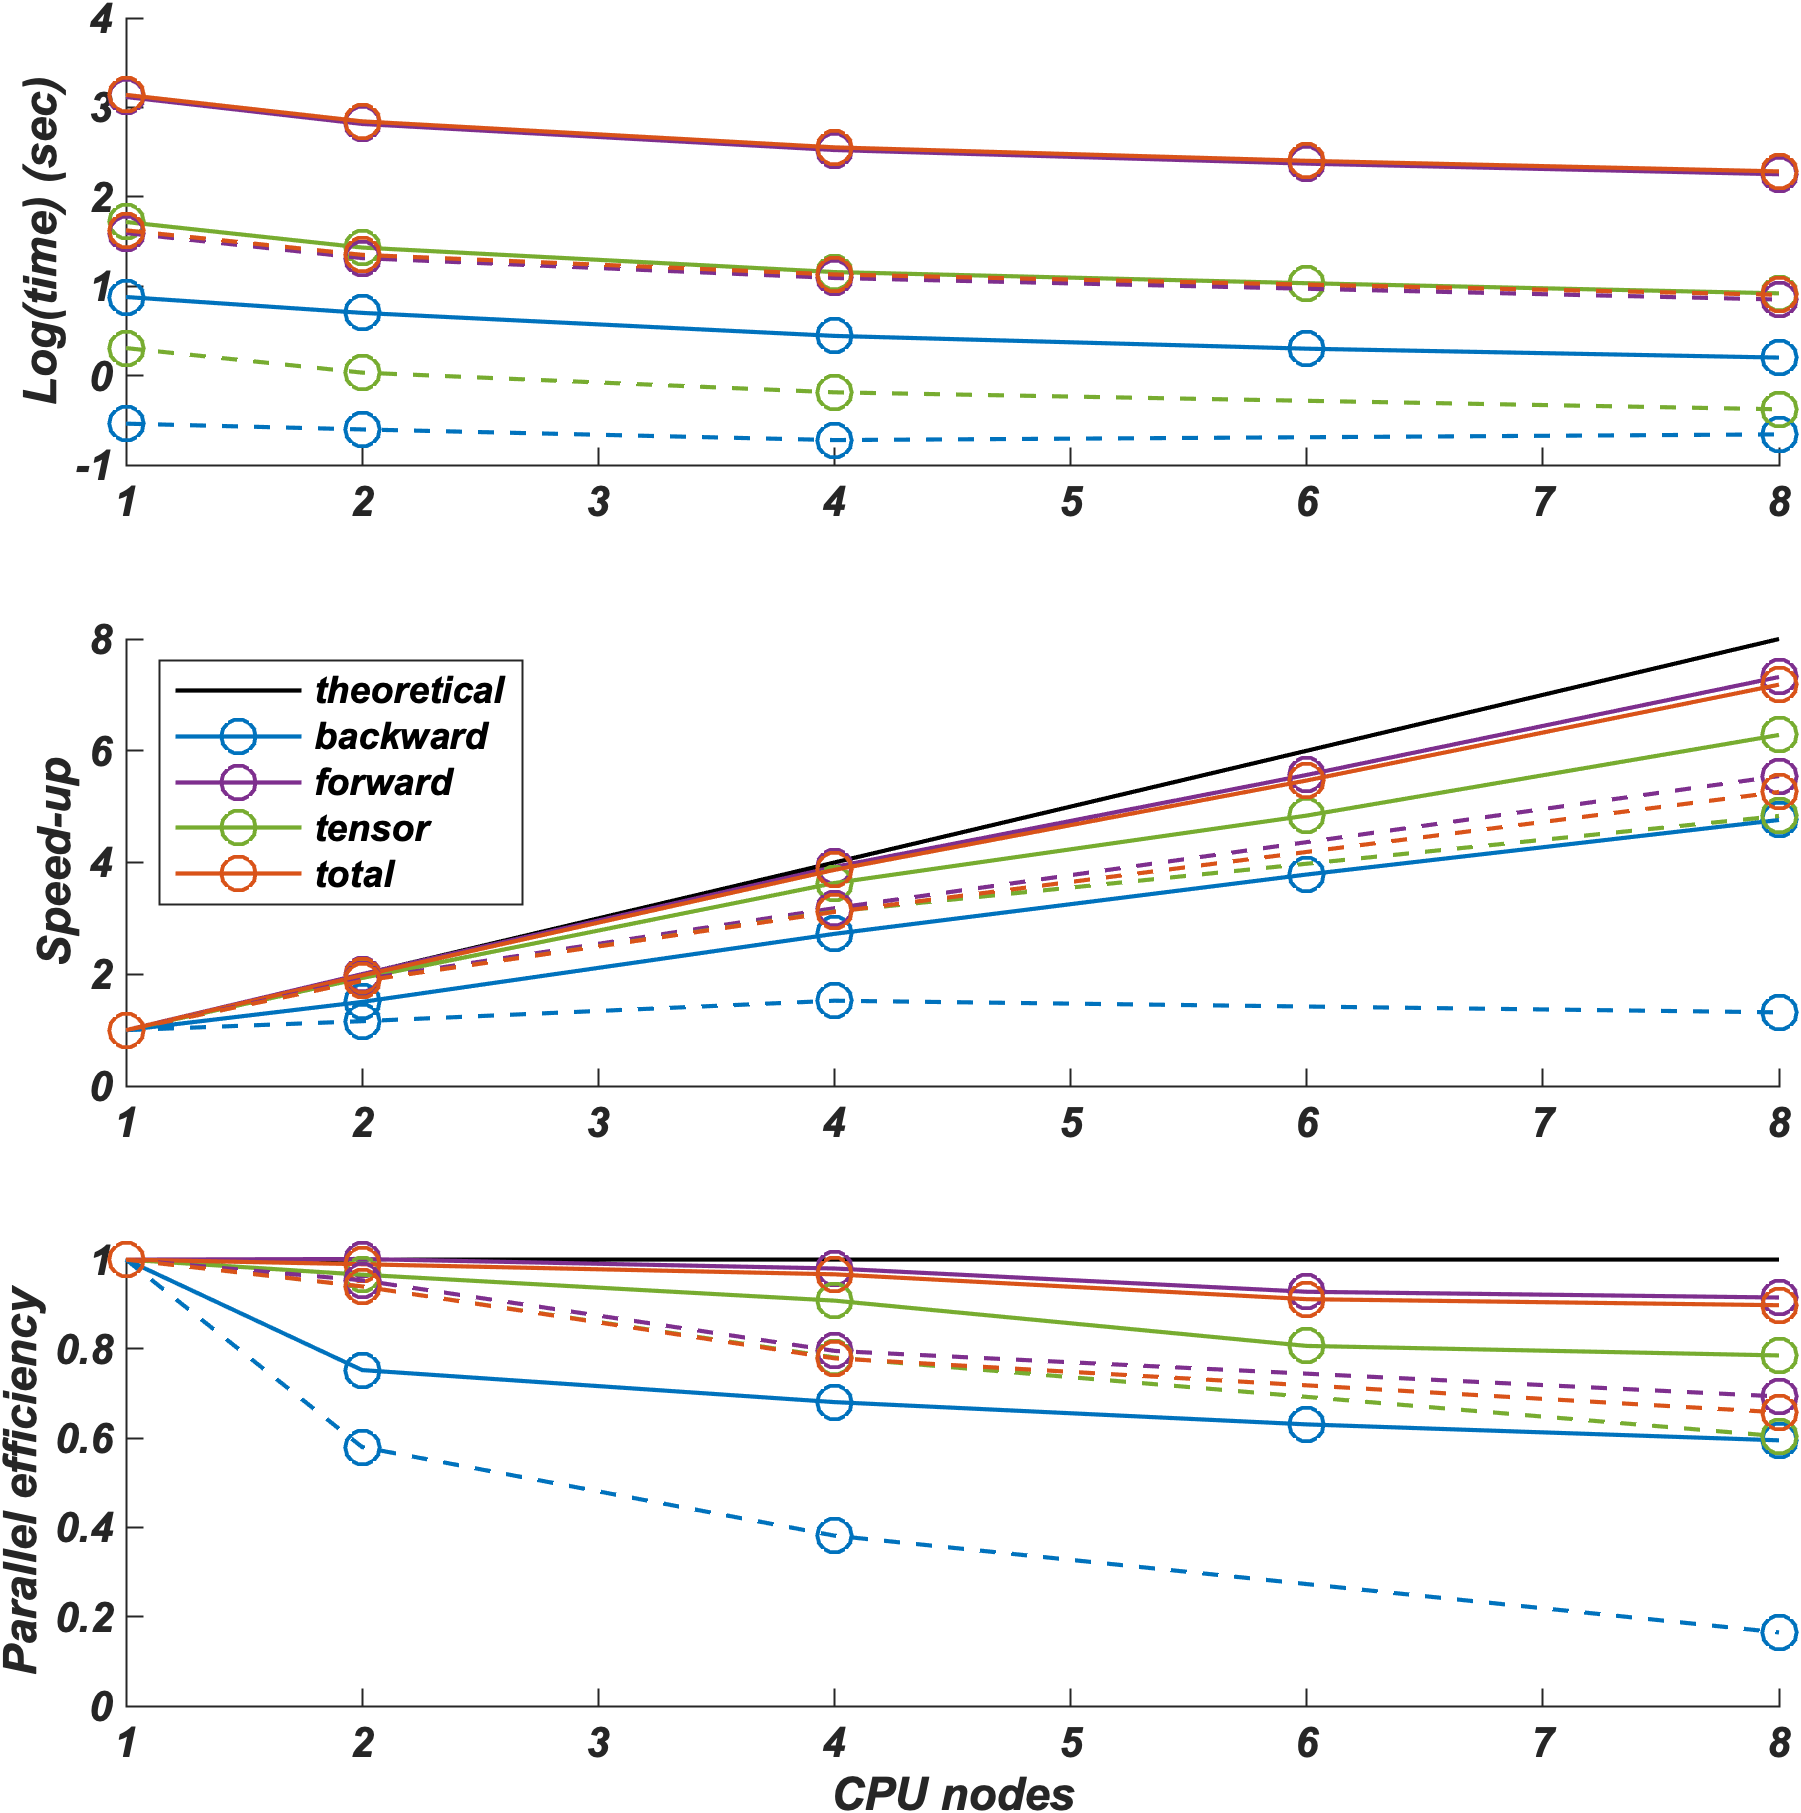
\includegraphics[width=0.8\textwidth]{DREX_M/drexm_time_speedup_scalability_log10.png}
    \caption{Runtime (top), speedup (centre) and parallel efficiency (bottom) of \drexmtitle{} for initial backward advection of aggregates (backward), forward advection and update of the LPO and Fij tensor (forward), full elastic tensor computation and output generation (tensor), and entire run (total). Results shown for two models included in the cookbooks: a 3D global convection model (steady-state flow, 96 timesteps, 1327606 aggregates, LPO computed only for 260474 upper mantle aggregates) and the 3D sinking slab model (dashed lines; time-dependent flow, 20 timesteps, 38509 aggregates, LPO computed for 25177 upper mantle and 6587 upper mantle transition zone aggregates). Runs performed on a HPE Superdome Flex (8 CPUs, 28 cores Intel Xeon(R) PLATINUM 8180 @ 2.50GHz) using from 1 to 8 nodes.
    }
    \label{fig:scalability}
\end{figure}

\vfill % Fill the rest of the page with whitespace
\chapter{\exevtitle: extrinsic elastic and viscous anisotropy}

\label{chapter:exev}

The \exevtitle{} software includes routines to compute extrinsic (SPO-related) fabrics and associated elastic and viscous tensors through effective medium theories\\

\section{Effective Medium Theories}

\subsection{Smoothed Transversely Isotropic Long-Wavelength Equivalent (STILWE)}
Introduced by \citep{backus1962jgr}, the STILWE is widely used to estimate the elastic properties of a stack of isotropic layers whose thickness is much smaller than the seismic wavelength. The equivalent elastic moduli of the homogeneous transversely isotropic medium are algebraic combinations of algebraic combinations of two elastic parameters ($\lambda$, $\mu$ or $\theta=Vs^2/Vp^2$). For a VTI medium, the elastic constants can be computed by using averages $\langle \cdot \rangle$ of $\mu$ and $\theta$ as \citep{backus1962jgr}:

\begin{gather}
    A=4(N-S)+R^{-1} (1-2T)^2\\
    C=R^{-1}\\
    F=R^{-1} (1-2T)\\
    L=\langle1/\mu \rangle^{-1}\\
    N=\langle\mu\rangle
\end{gather}

where $R=\langle \theta/\mu \rangle$, $S=\langle \theta\mu \rangle$, $T=\langle \theta \rangle$
The range of $\mu$ and $\theta$ for which the STILWE is stable is $0\leq\theta\leq3/4$ and $0\leq\mu\leq\ +\infty$.\\




\subsection{Differential Effective Medium (DEM) Theory}
The tensorial formulation for DEM is \citep{mclaughlin1977}:

\begin{align}
    \frac{d\mathbf{C^{DEM}}}{dV}&=\frac{1}{1-V}(\mathbf{C}-\mathbf{C^{DEM}})\mathbf{A^i}\\
    \mathbf{A^i}&=[\mathbf{I}+\mathbf{G^s}(\mathbf{C^i}-\mathbf{C^{DEM}} )]^{-1}
\end{align}

where $\mathbf{C^i}$ and $\mathbf{C^{DEM}}$ are the 4th-order elastic tensors of the inclusion and of the effective medium, respectively, $V$ is the volume fraction of the inclusion, $\mathbf{A^i}$ is the ratio of strain inside the inclusion to the strain in the host medium, $\mathbf{I}$ is the symmetric fourth-rank unit tensor, $\mathbf{G^s}$ is the symmetric Green’s interaction tensor \citep{mainprice1997tect},\citep{hornby1994}:

\begin{gather}
    G_{ijkl}^s=\frac{1}{2}(G_{ikjl}+G_{jkil})\\
    G_{ijkl}=\frac{1}{4\pi} \int_{0}^\pi sin(\theta) d\theta \int_{0}^{2\pi} (K_{ij}^{-1}x_k x_l) d\phi 
\end{gather}

Here, the Green’s interaction tensor G depends on the inclusion geometry and matrix elastic tensor through the Christoffel stiffness tensor $K_{ik} (x)=C_{ijkl}^{DEM} x_j x_l$ and directions $x_1=sin\theta cos\phi/a_1$, $x_2=sin\theta sin\phi/a_2$  and $x_3=cos\theta/a_3$, where $a_1$,$a_2$,$a_3$ are the semiaxes of the ellipsoidal inclusion.
Eq. S3.2.1a is solved with a 1st–order in time, 4th-order in space Runge-Kutta method by setting the matrix as the initial effective medium and then by progressively increasing the volume fraction of the inclusion. It is important to note that, for any inclusion concentration, the host medium is always fully interconnected while the inclusions remain isolated.

The DEM solution for an aggregate of spherical inclusions is shown in Fig. \ref{fig:dem_benchmark}, and benchmarked with the analytical solution \citep{mclaughlin1977}:

\begin{center}
$\frac{dK}{dV}=\frac{K-K^{DEM}}{1-V}\frac{K+K^\star}{K^{DEM}+K^\star}$

$\frac{d\mu}{dV}=\frac{\mu-\mu^{DEM}}{1-V}\frac{\mu+\mu^\star}{\mu^{DEM}+\mu^\star}$

where $K^\star=\frac{4}{3}\mu$, $\mu^\star=\frac{1}{6}\mu\frac{9K+8\mu}{K+2\mu}$
\end{center}

\begin{figure}[ht]
    \centering
    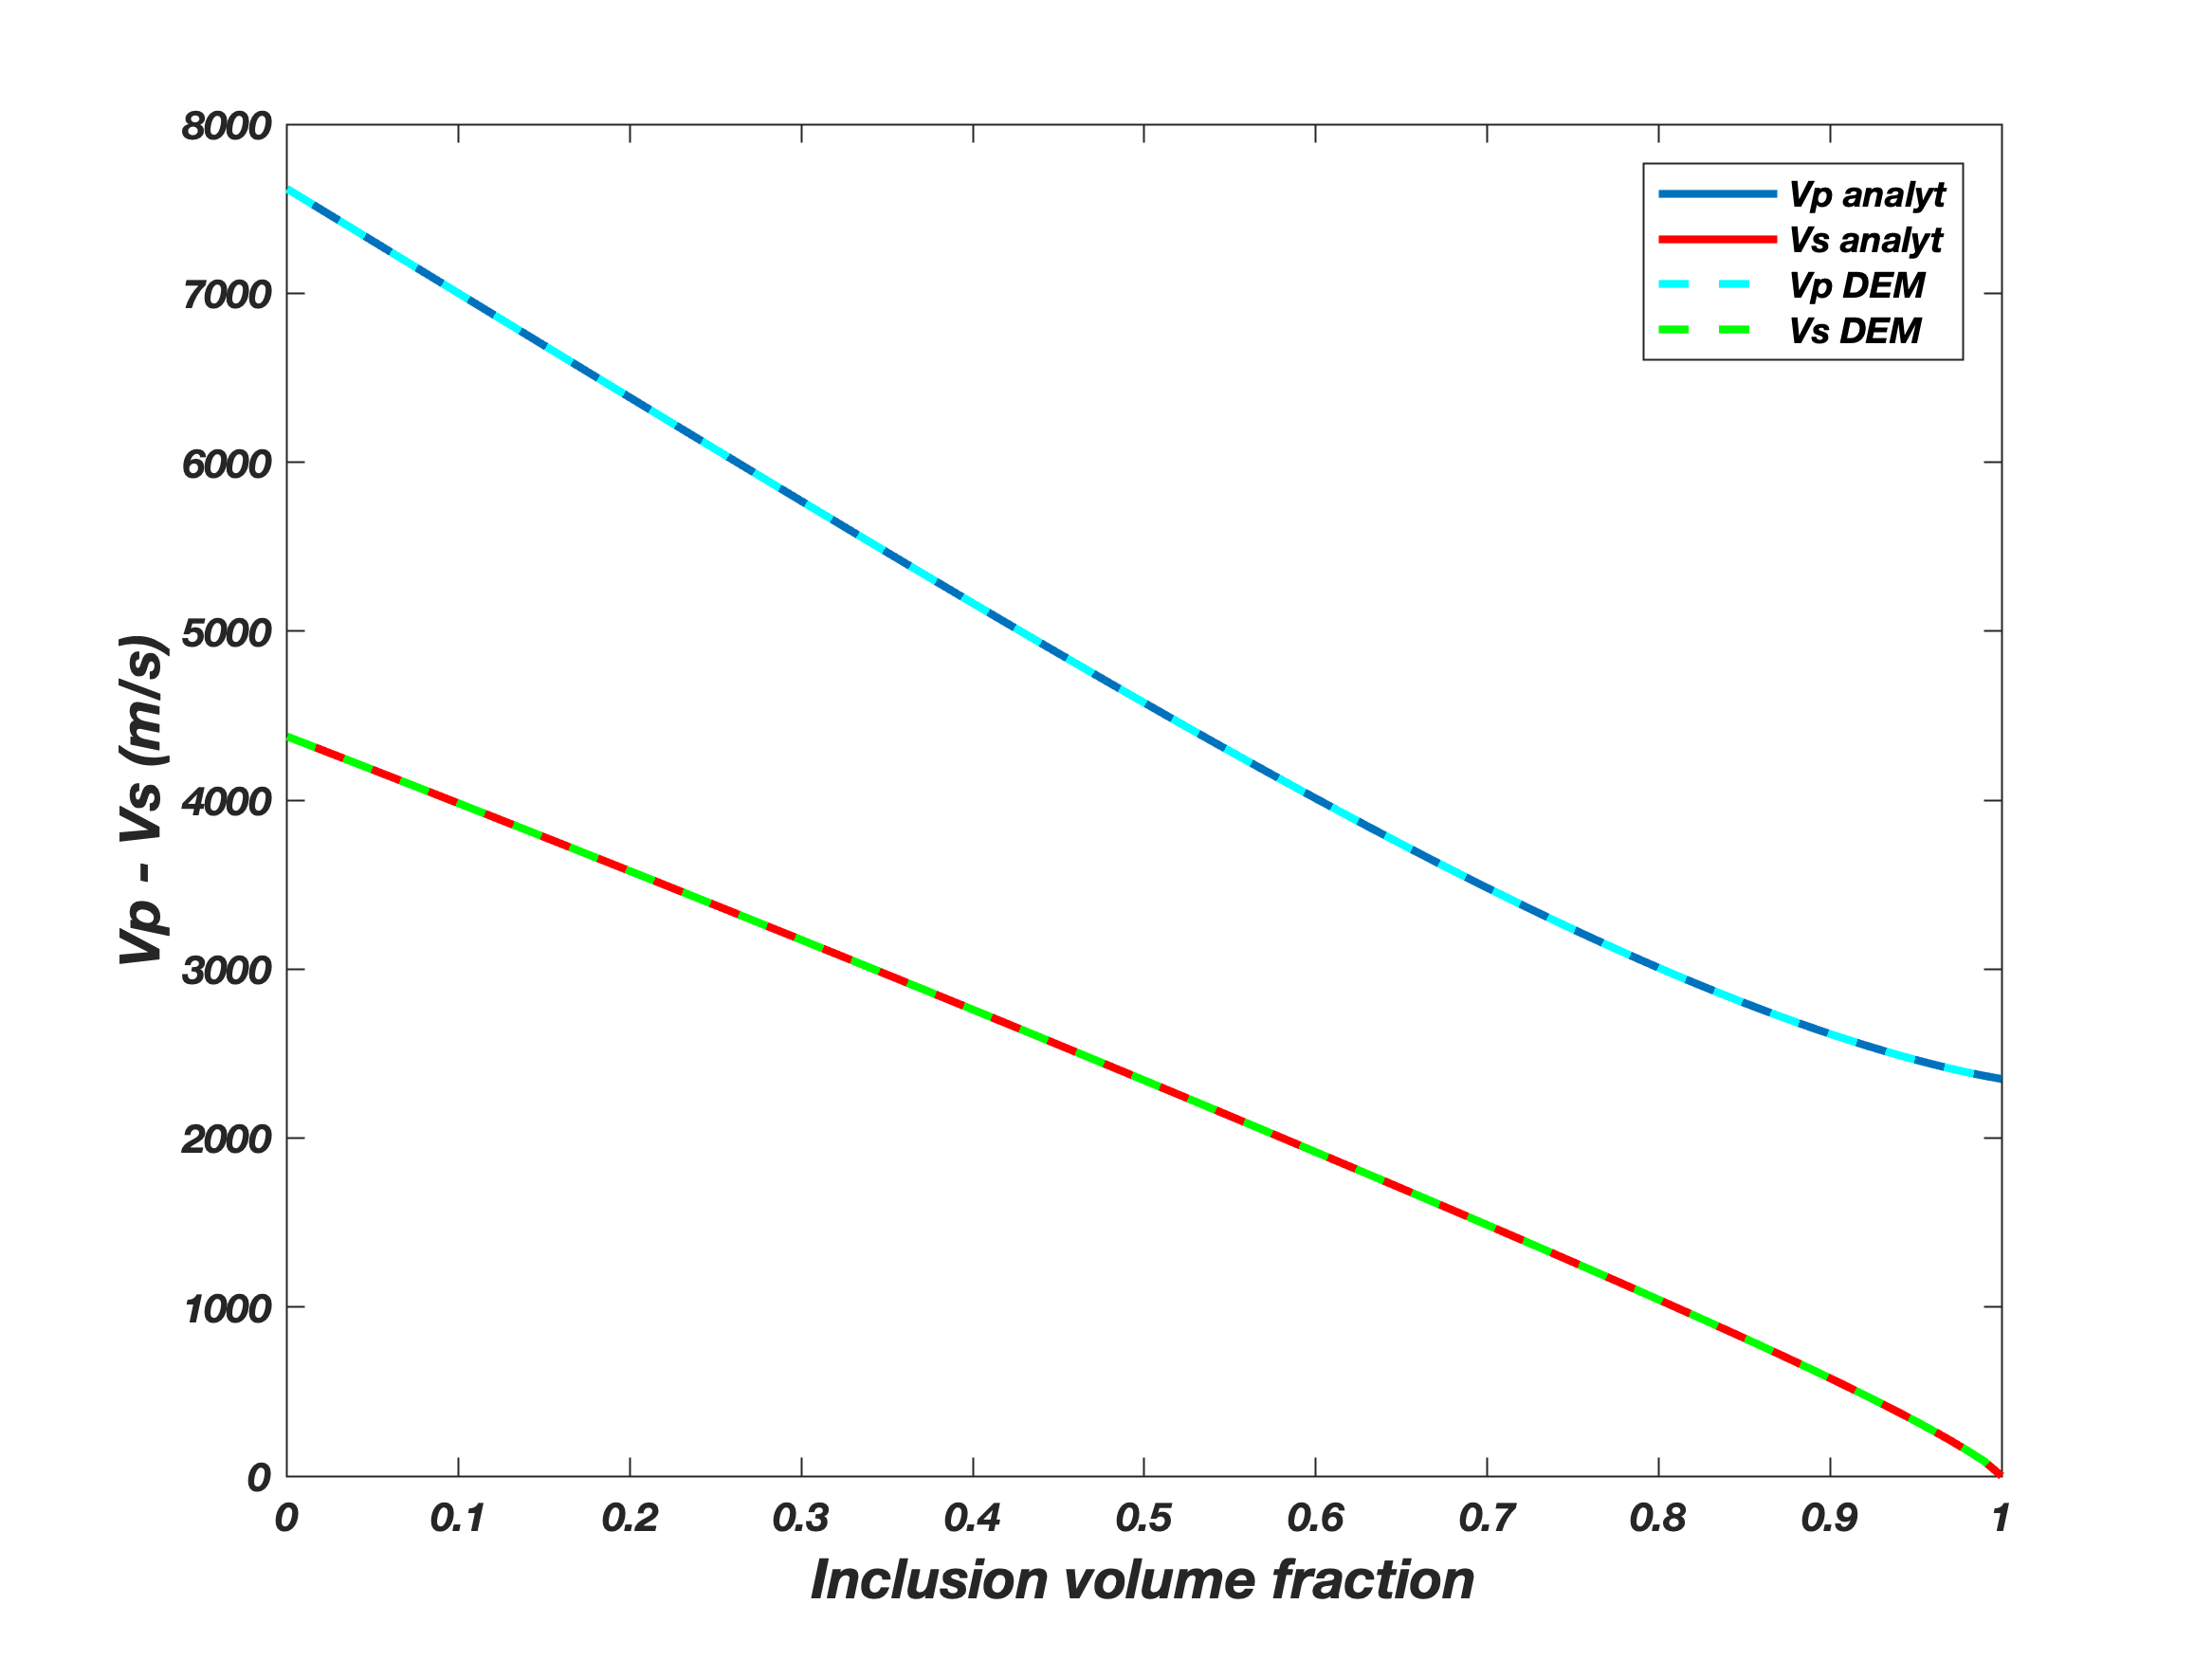
\includegraphics[width=1.0\textwidth]{EXEV/DEM_spheres.png}
    \caption{Comparison between analytical and DEM modeling solutions for spherical inclusions}
    \label{fig:dem_benchmark}
\end{figure}


\section{Extrinsic elastic anisotropy}
\label{section:elasticSPO}
Seismic anisotropy can be generated by the strain‐induced lattice preferred orientation (LPO) of minerals with anisotropic elastic properties (as modelled with D-Rex) and/or by the shape‐preferred orientation (SPO) of isotropic compositional heterogeneities. The former anisotropy is referred to as intrinsic mechanical anisotropy, while the latter is referred to as extrinsic mechanical anisotropy. Extrinsic anisotropy occurs when (i) the size of the SPO is much smaller than the wavelength of the seismic signal and (ii) the contrast in isotropic elastic properties between the compositional domains is very large. When these conditions are satisfied, seismology fails to distinguish a finely layered and strongly heterogeneous isotropic medium from a smooth intrinsic anisotropic medium.\\
Within the Earth, extrinsic anisotropy can be related to either (1) the presence of a free gas or liquid phase included in elongated and preferentially oriented grain boundaries, pores, cracks, and porosity bands or (2) grain‐scale (micrometer to centimeter) and/or rock‐scale (centimeter to kilometer) SPO of compositionally distinct domains.\\*
\\
Modelling of extrinsic elastic anisotropy due to SPO is activated with parameter \fonts{spomod} in \texttt{drexs\_input.dat} (when using \drexstitle{})  or \texttt{viztomo\_input.dat} (when using \viztomotitle{}):
\begin{itemize}
    \item[] \fonts{0} = no extrinsic anisotropy is computed, and the original elastic tensor computed as a function of the LPO evolution is retained.
    
    \item[] \fonts{1} = extrinsic elastic anisotropy computed with the STILWE (Smooth Transversely Isotropic Long-Wavelength Equivalent medium; \citep{backus1962jgr}), which calculates the elastic properties for a layered medium with $\geq$ 2 materials. The original elastic tensor computed in \drexmtitle{} is ignored. The newly computed elastic tensor is then rotated with the layering normal to the shortest semiaxis of the FSE (e.g., \citet{olson1984jgr}).
    
    \item[] \fonts{2} = extrinsic elastic anisotropy computed with the DEM (Differential Effective Medium; \citep{mclaughlin1977,mainprice1997tect}), which calculates the elastic properties of a 2-phase matrix-inclusions system. The shape of the inclusions is ellipsoidal and can be defined in \texttt{spo\_input.dat} together with their volume fraction. The elastic tensors of the 2 media are constant and the original elastic tensor computed in \drexmtitle{} is ignored. The inclusions are oriented parallel to $\sigma_1$, the maximum deviatoric stress, and normal to $\sigma_3$, the minimum deviatoric stress, $\pm$ an angle defined by \fonts{phi\_spo}.

    \item[] \fonts{3} = same as \fonts{spomod = 2}, but the elastic tensor computed in \drexmtitle{} is retained for the matrix.
\end{itemize}


In \viztomotitle{} the SPO fabrics are computed for aggregates with ln\textsubscript{fse} $\geq$ \fonts{ln\_fse\_min}, implying that the rocks have accumulated a certain amount of deformation to generate the SPO fabrics. \\
In order to have the possibility to compute seismological synthetics (e.g., SKS-splitting) with the new elastic tensors, these are saved in a \cijkltitle{} file placed in a new directory \fonts{output\_dir}\texttt{/SPO/}.\\

\subsection{STILWE modeling (active when \fonts{spomod = 1})}
The STILWE can be used to model grain-/rock-scale layering when the P-T conditions of each aggregate are known (implying that the geodynamic model is thermo-mechanical and that \fonts{ptmod > 0} when running \drexmtitle, or \drexstitle). Grain-scale or rock-scale layering can be evaluated for 5 lithologies with lookup tables of density and isotropic elastic moduli f(P,T) generated with MMA\_EoS \citep{chust2017jgr}. It is possible to simultaneously compute grain-scale and rock-scale SPO by setting \fonts{spograinmod > 0} and choosing a rock mixture in volfractrock.
When \fonts{ptmod = 0}, the constant C\textsubscript{$\alpha\beta$} of Medium 1 and 2 defined in \texttt{spo\_input.dat} will be used with a relative volume fraction \fonts{Vmax} for Medium 2. \\*
When using the STILWE, the LPO fabrics are ignored.\\*
The SPO modeling parameters to be set in \texttt{spo\_input.dat} are the following:\\
\\
Set type of layered model:
\begin{itemize}
    \item \fonts{spograinmod}: when > 0, computes the grain-scale SPO for a single lithology or lithology mixture as indicated in volfractrock. The allowed lithologies are Harzburgite, Pyrolite, Basalt and Pyroxenite, as Dunite does not generate grain-scale SPO.  The sum of volfractrock must be 100 (\%). It requires \fonts{spomod = 1}, \fonts{ptmod > 0} and \fonts{sporockmod = 0}.
    \item \fonts{sporockmod}: when > 0, computes the rock-scale SPO for the lithology mixture indicated in volfractrock. The sum of volfractrock must be 100 (\%) and there should be $\geq$2 lithologies with volfractrock > 0. It requires \fonts{spomod = 1}, \fonts{ptmod > 0} and \fonts{spograinmod = 0}.
    \item \fonts{volfractrock(1,…,5)}: volume fractions in \% of the 5 different lithologies (\fonts{1}: Dunite; \fonts{2}: Harzburgite; \fonts{3}: Pyrolite; \fonts{4}: Basalt; \fonts{5}: Pyroxenite). The sum must be 100\%.
\end{itemize}

\subsection{DEM modelling (active when \fonts{spomod > 1})}
The presence of a liquid phase (i.e., with null shear modulus) must be always evaluated with the DEM model (\fonts{spomod = 2} or \fonts{3}), as using the STILWE produces infinite elastic anisotropy.\\
As the inclusions are oriented relative to the principal stresses, when using \viztomotitle{} the flow field \textbf{V} from the input \vtptitle{} file needs to be loaded. As such, a copy of the "present-day" \vtptitle{} (where * is given by \fonts{Tend} as defined in \texttt{viztomo\_input.dat}) must be placed in \fonts{cijkl\_dir}.\\
When using the DEM, the matrix elastic tensor can be the constant C\textsubscript{$\alpha\beta$} of Medium 1 (\fonts{spomod = 2}) or the one from the \drexmtitle{} strain-induced LPO modeling (\fonts{spomod = 3}). \\
The inclusions elastic tensor is always given by the constant C\textsubscript{$\alpha\beta$} of Medium 2, and their volume fraction is given either by \fonts{Vmax} or, when \fonts{meltspomod > 0}, by the porosity of the geodynamic model (see Figs. \ref{fig:meltviscosity}, \ref{fig:extrinsic_anisotropy}). \\
The SPO modeling parameters to be set in \texttt{spo\_input.dat} are the following (unless otherwise specified, the variable format is \texttt{double precision}):\\
\\
Assign geodynamic model porosity (valid only when using \viztomotitle{} and not for the single aggregate fabric modelled with \drexstitle):
\begin{itemize}
    \item \fonts{meltspomod}: (Integer) when > 0, it requires an input file from which the porosity distribution in the computational domain is loaded. The inclusions volume fraction is given by the loaded fluid/melt fraction interpolated to the aggregate position.
    \item \fonts{meltfilename}: (String) name of the input HDF5 file with the geodynamic model porosity distribution. This file must be located in \fonts{cijkl\_dir} and can be created with \texttt{/VIZTOMO/makeporosityfile.m}.
\end{itemize}
Set constant elastic tensors (in Voigt notation) and density for the 2 media:
\begin{itemize}
    \item \fonts{Cback}: constant C\textsubscript{$\alpha\beta$} moduli of Medium 1 (Matrix for DEM)
    \item \fonts{Cinc}: constant C\textsubscript{$\alpha\beta$} moduli of Medium 2 (Inclusions for DEM)
\end{itemize}
Set DEM parameters:
\begin{itemize}
    \item \fonts{esa1,esa2,esa3}: define shape of the ellipsoidal inclusions defining the relative length of the 3 semiaxes ( or better to sigma 1, 2, 3). These semiaxes coincide initially with axes 1, 2 and 3 and then rotated such that \fonts{esa1} and \fonts{esa3} are parallel to, respectively, $\sigma_1$ and $\sigma_3$. The aspect ratio should not exceed 1000.
    \item \fonts{Vmax}: maximum inclusions volume fraction ( \fonts{0 < Vmax < 1})
    \item \fonts{Vstp}: volume fraction increments of the inclusions in the DEM model. The larger \fonts{Vstp}, the less accurate is the computation. \fonts{Vstp} should not be larger than 0.01. 
\end{itemize}
Cracks/porosity bands orientation relative to $\sigma_1$:
\begin{itemize}
    \item \fonts{phi\_spo} (\fonts{$\phi\textsubscript{SPO}$}): when different from 0, it allows to rotate around $\sigma_2$ the fluid-filled cracks/porosity bands by an angle  (in $^{\circ}$) with respect to $\sigma_1$ and in the direction of vorticity. As an example, porosity bands in melt-bearing mantle samples forming at relatively large strain are orientated at about $-25^{\circ}$ from $\sigma_1$ during simple shear deformation (the minus sign means that the rotation is against the vorticity) (\citet{katz2006} and references therein).
\end{itemize}



See \ref{table:spo} for the different combinations of SPO model parameters, and Fig \ref{fig:extrinsic_anisotropy} for an application to a 2D oceanic ridge setting.

The program \texttt{/EXEV/DEMelastic/DEMelastic.f90} can be used to compute the two-phase component elastic properties for a range of inclusion ellipsoidal shapes and volume fractions as defined in \texttt{/EXEV/DEMelastic/dem\_input.dat} (\texttt{COMPILE: ./bash\_compile},
 \texttt{RUN: ./demelastic}). \\
The elastic tensors properties saved in file \texttt{elastictensordem.h5} can then be plotted in Flinn diagrams using \texttt{/EXEV/DEMelastic/readDEMelastic.m} (Fig. \ref{fig:dem_elastic}).

\begin{figure}[ht]
    \centering
    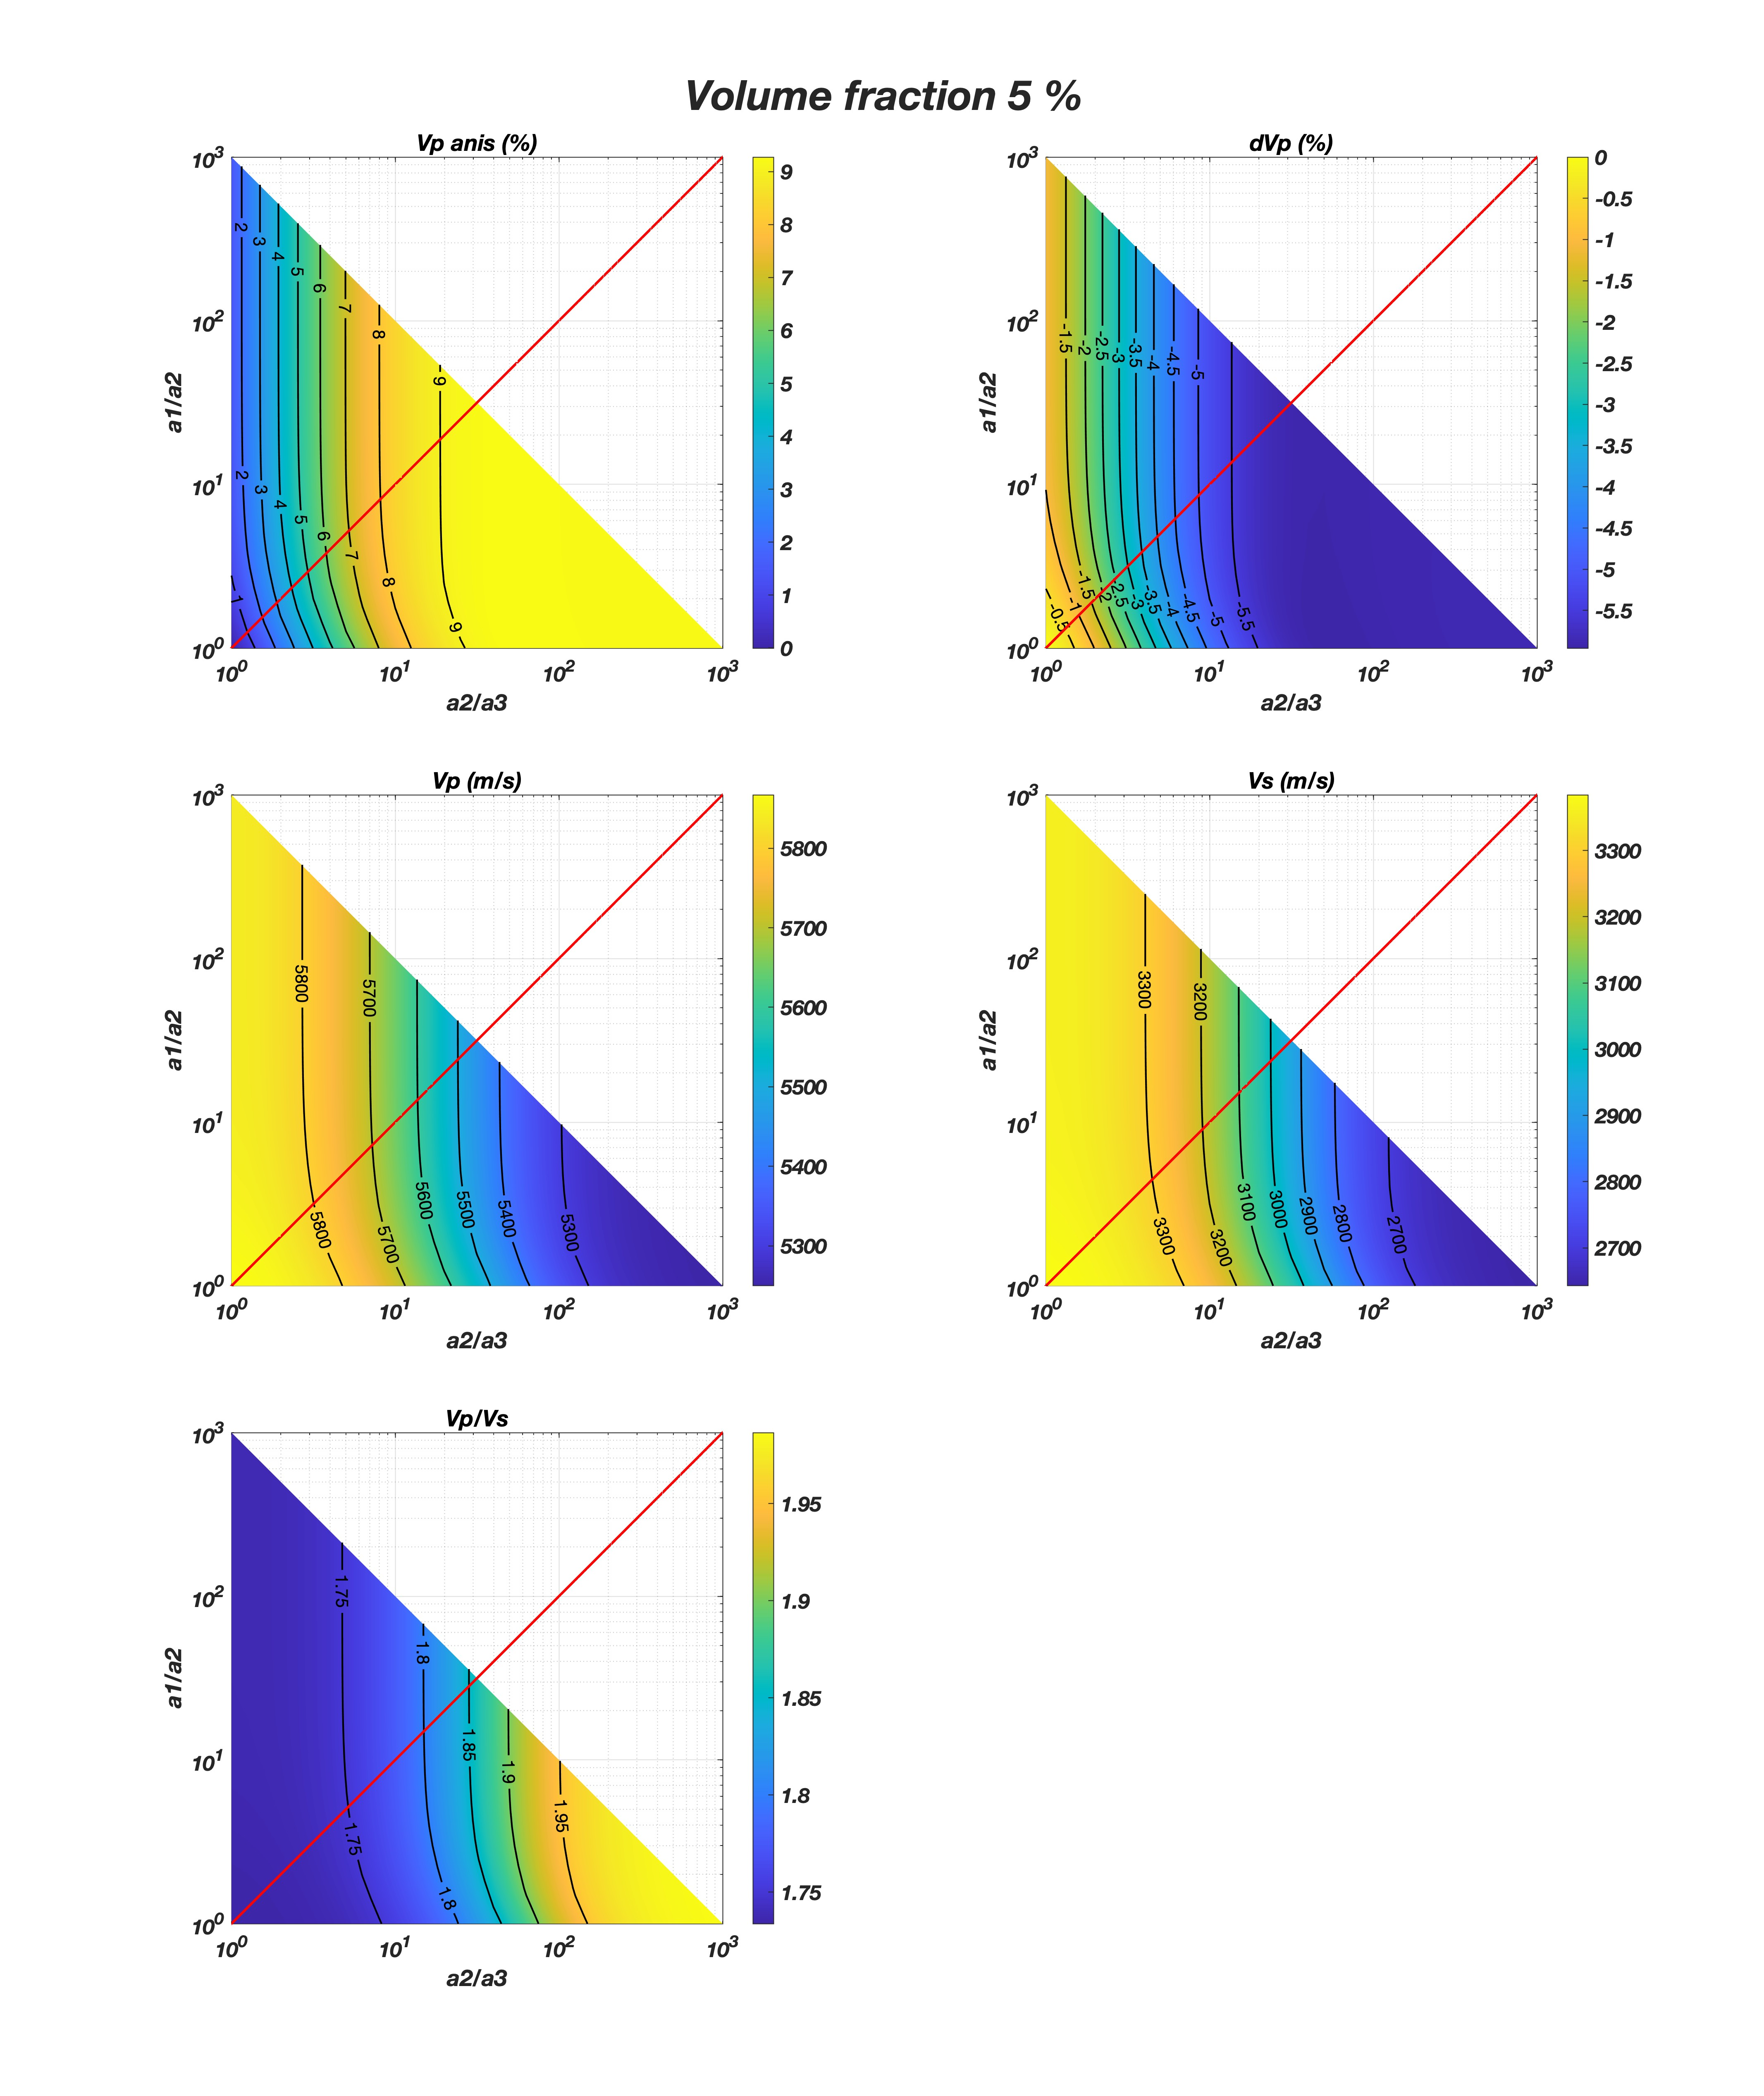
\includegraphics[width=0.82\textwidth]{EXEV/dem_elastic0.05.jpg}
    \caption{Flinn diagram showing the elastic properties of an aggregates with $5\%$ in volume of melt-filled ellipsoidal inclusions with different shapes defined by the semiaxes ratios a1/a2 and a2/a3 and matrix-inclusion physical properties as defined in \texttt{dem\_input.dat}. From top to bottom, left to right: P-wave anisotropy, isotropic P-wave anomaly w.r.t. the dry sample, isotropic P- and S-wave velocities, and their ratio.}
    \label{fig:dem_elastic}
\end{figure}

\newpage

\begin{table}[ht]
\centering
\caption{\raggedright Different SPO models as a function of operating mode parameters}
\begin{adjustbox}{width=1\textwidth}
\begin{tabular}{|>{\centering}m{.09\textwidth}|>{\centering}m{0.09\textwidth}|>{\centering}m{0.16\textwidth}|>{\centering}m{0.16\textwidth}|>{\centering}m{0.15\textwidth}|m{0.35\textwidth}|} 

\hline
\fonts{spomod}	& \fonts{ptmod}$^1$	& \fonts{spograinmod} &	\fonts{sporocksmod} &	\fonts{meltspomod}	& Type of model\\ [1ex] 
\hline\hline

 \fonts{1} & \fonts{0} & - & - & - & STILWE with 2 constant C\textsubscript{$\alpha\beta$} from \texttt{spo\_input.dat} \\\hline

\fonts{1} &	\fonts{1} & \fonts{1} & \fonts{0} & - & \small{STILWE with grain-scale SPO f(P,T)} \\\hline
\fonts{1} & \fonts{1} & \fonts{0} & \fonts{1} & - & STILWE with rock-scale SPO f(P,T)\\\hline
\fonts{2} & - & - & - & \fonts{0} & DEM with constant C\textsubscript{$\alpha\beta$}, ellipsoidal shape and $\psi^2$ = \fonts{Vmax} from \texttt{spo\_input.dat} \\\hline
\fonts{2} & - & - & - & \fonts{1} & DEM with constant C\textsubscript{$\alpha\beta$} and ellipsoidal shape from \texttt{spo\_input.dat}. $\psi$ from geodynamic model\\\hline
\fonts{3} & - & - & - & \fonts{0} & DEM with C\textsubscript{$\alpha\beta$} from LPO for matrix, while constant C\textsubscript{$\alpha\beta$} for inclusions, ellipsoid shape and $\psi$ = \fonts{Vmax} defined in \texttt{spo\_input.dat}\\\hline
\fonts{3} & - & - & - & \fonts{1} & DEM with C\textsubscript{$\alpha\beta$} from LPO for matrix, while constant C\textsubscript{$\alpha\beta$} for inclusions, ellipsoid shape defined in \texttt{spo\_input.dat}. $\psi$ from geodynamic model\\
\hline
\hline

\end{tabular}

\end{adjustbox}

\raggedright \footnotesize{$^1$ to be set in the \texttt{drexs\_input.dat} or \texttt{viztomo\_input.dat} files.}\\
\raggedright \footnotesize{$^2$ porosity.}\\
\vspace{0.3cm}

\raggedright \footnotesize{The '-' symbol means that the corresponding parameter is ignored}


\label{table:spo}
\end{table}

\newpage

\section{Extrinsic viscous anisotropy}
The modelling of extrinsic viscous anisotropy related to rock-scale and grain-scale fabrics relies on the DEM modelling and a geometric parametrization extrapolated from 3D high-resolution simulations of deforming matrix-inclusions aggregates \citep{demontserrat2021}. \\
The DEM modelling is used to generate a database of viscous tensors for different matrix-inclusions viscosity contrasts, relative volume fraction and inclusions aspect ratios. Given the aggregate bulk FSE, the geometric parametrization provides an estimate of the inclusions average aspect ratio and orientation, thus allowing the mapping of the viscous tensor from the database and its rotation with respect to the FSE axes orientation. \\
Thus, the first modelling phase requires generating the DEM database (stored in file \texttt{viscoustensordem.h5}), which, together with the geometric parametrization, can be then exploited to estimate the local viscous tensor due to SPO-related fabrics in every point of the computational domain. The viscous tensor can be returned on the fly when the proper functions are called from a running geodynamic model (coupled mechanical simulations). Alternatively, its anisotropic properties can be computed for post-processing visualization (uncoupled mechanical simulations).\\
It is important to note that the values of the aggregate viscous tensor are always normalized with respect to the isotropic matrix viscosity $\eta_{mat}$. Hence, to retrieve the total viscous tensor:

$\pmb{\eta_{tot}}= \pmb{\eta_{DEM}}\cdot\eta_{mat}$


\subsection{Generate the viscous tensor database}
\label{section:viscousDEM}

The main file \texttt{DEMviscous.f90} can be compiled and run as:

\texttt{DIRECTORY: /EXEV/DEMviscous}\\*
\\
\texttt{COMPILE: ./bash\_compile}\\*
\\
\texttt{RUN: ./demviscous}\\*

The DEM modeling parameters to be set in the parameter input file \texttt{dem\_input.dat} are the following (unless otherwise specified, the variable format is \texttt{double precision}):
\begin{itemize}
    \item \fonts{devmod}: (Integer) 
    \begin{itemize}
        \item[] \fonts{0} = compute total viscous tensor
        \item[] \fonts{>0} = compute deviatoric viscous tensor
    \end{itemize}
\end{itemize}

Set viscosities for the 2 media:
\begin{itemize}

    \item \fonts{isotropicmod}: (Integer)  
    \begin{itemize}
        \item[] \fonts{0} = viscous tensors as defined in Voigt notation by \pmb{$\eta_{mat}$} and \pmb{$\eta_{inc}$}
        \item[] \fonts{>0} = force the viscous tensors to be isotropic with the range of viscosity contrasts defined by \fonts{etacontrmin}, \fonts{etacontrmax}, \fonts{etacontrstp}
    \end{itemize}
    \item \fonts{etacontrlogscalemod}: (Integer), when > 0, the following viscosity contrasts must be defined as $log_{10}$.
    \item \fonts{etacontrmin}, \fonts{etacontrmax}, \fonts{etacontrstp}: define min, max and increment of isotropic viscosity contrasts.
    
    \item \pmb{$\eta_{mat}$}: $\eta_{\alpha\beta}$ moduli of Medium 1 (Matrix for DEM)
    \item \pmb{$\eta_{inc}$}: $\eta_{\alpha\beta}$ moduli of Medium 2 (Inclusions for DEM)

\end{itemize}

Define inclusions shape range:
\begin{itemize}
    \item \fonts{axislogscalemod}: (Integer), when > 0, the following semiaxes lengths must be defined as $log_{10}$.
    \item \fonts{esa1,esa2,esa3}: define shape of the ellipsoidal inclusions defining the range of lengths for, respectively, the maximum, intermediate, minimum semiaxes normalized to that of the smallest one. Thus, \fonts{esa3}, the length of semiaxis 3, should be always 1. The range of lengths should be given as the min. max. and increment lengths.
\end{itemize}
    
Define array of inclusions volume fraction for which the viscous tensor is saved:
\begin{itemize}
    \item \fonts{Volsavemin}: minimum inclusions volume fraction ( \fonts{0 < Volsavemin < Vsavemax}). It must be a multiple of \fonts{Vstpdem}.
    \item \fonts{Volsavemax}: maximum inclusions volume fraction ( \fonts{Volsavemin < Volsavemax < 1}). It must be a multiple of \fonts{Vstpdem}.
    \item \fonts{Volsavestp}: volume fraction increments of the inclusions in the DEM model. It must be a multiple of \fonts{Vstpdem}. 
\end{itemize}

Set volume fraction increment for DEM solution
\begin{itemize}
    \item \fonts{Vstpdem}: it is recommended to keep it as low as possible, especially for large aspect ratios, as the larger \fonts{Vstpdem}, the less accurate is the computation. However, bear in mind that the smallest the volume increment, the larger the number of iterations and the longer the computational time. As a rule of thumb, \fonts{Vstpdem} should not be larger than 0.01, and a good choice is 0.005.
\end{itemize}

The viscous tensor database is saved in the output file \texttt{EXEV/DEMviscous/viscoustensordem.h5} that must be then copied/moved in the \vizvisctitle{} directory.

The viscous tensors properties saved in file \texttt{viscoustensordem.h5} can then be plotted in Flinn diagrams using \texttt{/EXEV/DEMviscous/readDEMviscous.m}.

\\
In \texttt{VIZVISC/viscoustensordem.h5} we provide such a database for deviatoric viscous tensors that can be readily used and computed in the parameter ranges:\\* 
\\
$log_{10}(etac)=-3:1:3$,\\
$log_{10}(esa1)=0:0.1:3$,\\
$log_{10}(esa2)=0:0.1:3$,\\
$log_{10}(esa3)=0$,\\
$Volume fraction = 0.05:0.05:0.3$.
\vfill{}

\subsection{Coupled mechanical simulations}

\texttt{DIRECTORY: /EXEV}\\*

In order to update the \textbf{F} tensor and extract the associated \pmb{$\eta$} tensor from the database, the file \texttt{viscoustensor.f90} must be compiled together with \texttt{moduledem.f90}. This file includes subroutine \texttt{viscoustensor()} to be called from the large-scale geodynamic model by inputting the following variables:

\begin{itemize}
    \item[] \fonts{x1m} = axis 1 coordinate. In polar coordinates, longitude in radians (double)
    \item[] \fonts{x3m} = axis 3 coordinate. In polar coordinates, colatitude in radians (double). In 2D cylindrical/annulus, set to pi/2.0 
    \item[] \fonts{cartspher} = cartesian (1) or polar (2) domain (integer)
    \item[] \fonts{yinyang} = Yin-Yang grid for 3D global simulations, active when = 2 (integer)
    \item[] \fonts{fse0} = particle Fij (3x3 double) in cartesian coordinates       
    \item[] \fonts{l} = particle velocity gradient (3x3 double) in cartesian coordinates
    \item[] \fonts{dt} = timestep (double)                
    \item[] \fonts{etac} = matrix-inclusions isotropic viscosity contrast: $\eta_inc/\eta_mat$ (double). For hard inclusions (\fonts{etac} $ > 1$), allowed values are \fonts{etac}$ = 10, 100, 1000$
    \item[] \fonts{volinc} = inclusions volume fraction (double). Allowed values are \fonts{volinc} $= 0.1, 0.2, 0.3$.
\end{itemize}

The function returns as an output:
\begin{itemize}
    \item[] \fonts{fse}  = updated particle \textbf{F} tensor (3x3 double) in cartesian coordinates      
    \item[] \fonts{etavoigt} = mapped viscous tensor (6x6 double)
\end{itemize}


\vfill{}

\subsection{Uncoupled mechanical simulations: visualizing the viscous tensors with \vizvisctitle{}}

\texttt{DIRECTORY: /VIZVISC}\\*
\\
\texttt{COMPILE: ./bash\_compile}\\*
\\
\texttt{RUN: ./vizvisc vizvisc\_input.dat}\\*

\vizvisctitle{} is a software pretty much similar to \viztomotitle{}. It includes routines for post-processing the \cijkltitle{} output files generated with \drexmtitle{} and for visualizing the \pmb{$\eta$} anisotropy and \textbf{FSE} tensors with \paraviewtitle{}. The viscous tensor \pmb{$\eta$} due to extrinsic viscous anisotropy is extracted from a database of tensors according to the FSE geometry, the matrix-inclusions viscosity contrast (\fonts{etac}) and the inclusions volume fraction (\fonts{volinc}). Thus, pre-computation of the viscous tensor database as explained in section \ref{section:viscousDEM} is required before running \vizvisctitle{} (or one can use the one provided as explained above). The viscous anisotropy is visualized on an eulerian grid defined below, as a function of the radial and azimuthal viscous anisotropy (which are analogous to those defined for elastic anisotropy) computed in the FSE reference frame.

The parameter input file is \texttt{vizvisc\_input.dat}, where the following parameters can be set (unless otherwise specified, the variable format is \texttt{double precision}): 

A) Input and output directories/files
\begin{itemize}
    \item \fonts{cijkl\_dir}: (String) path to input directory where to load the \drexmtitle{} \cijkltitle{} output files (the path should end with  “/” )
	\item \fonts{output\_dir}: (String) path to output directory where to save the visualization output (the path should end with  “/” ), which can be or not the same as \fonts{cijkl\_dir}
	\item \fonts{Tinit},\fonts{Tstep},\fonts{Tend}: (Integers) initial, increment and final number of input \cijkltitle{} files to be processed. When \fonts{Tinit} = \fonts{Tend}, only a single \cijkltitle{} file is processed.
\end{itemize}

B) Define viscosity contrast and inclusions volume fraction
\begin{itemize}
    \item \fonts{etac}: isotropic viscosity contrast: $\eta_{inc}/\eta_{mat}$. For hard inclusions (\fonts{etac} $ > 1$), allowed values are \fonts{etac}$ = 10, 100, 1000$ 
	\item \fonts{volinc}: inclusions volume fraction. Allowed values are \fonts{volinc} $= 0.1, 0.2, 0.3$.
\end{itemize}

C) Visualize properties of Lagrangian aggregates:
\begin{itemize}
    
    \item \fonts{Lagrangian}: (Integer) when > 0, activates visualization of Lagrangian aggregates. The datasets saved in file \texttt{lagrangian*.h5} can be loaded on PARAVIEW with the corresponding file \texttt{XDMF.lagrangian*.xmf}. Vectors can be visualized applying the Glyph filter
	
	\item \fonts{ln\_fse\_min}: assumes values >= 0.0, and indicates the threshold of\\ ln\textsubscript{fse} = ln(fse\textsubscript{max}/fse\textsubscript{min}) above which aggregates properties are visualized. It allows to skip aggregates that experienced low deformation and are nearly isotropic (try with 0.5, for example, as suggested by \citet{becker2006epsl}). When  = 0.0, all aggregates are displayed.
	
	\item \fonts{uppermantlemod}: (Integer) when > 0, displays only upper mantle aggregates.
	
	\item \fonts{rocktypemod}: (Integer) when > 0, displays the rocktype of the aggregates.
	
	\item \fonts{fse3Dmod}\footnotemark: (Integer) when > 0, the left stretch tensor \textbf{FSE} of ALL aggregates are saved in file \texttt{3Dfse*.h5}, and can be loaded on \paraviewtitle{} with \texttt{XDMF.3Dfse*.xmf}. Applying the TensorGlyph filter, the 3D FSE are displayed. The ellipsoids can be colored according to the rocktype or fse\textsubscript{max} (suggestion: set the scale factor equal to the initial spacing of the aggregates defined in \texttt{drexm\_input.dat}) (see Fig. \ref{fig:polarcells_viscous}C).
	
	\item \fonts{fseminmod}: (Integer) when > 0, saves the fse\textsubscript{min} vector scaled by ln\textsubscript{fse}.
	
	\item \fonts{fsemaxmod}: (Integer) when > 0, saves the fse\textsubscript{max} vector scaled by ln\textsubscript{fse}.
	
\end{itemize}

\footnotetext{Visualizing the 3D ellipsoid requires lots of computer memory, so be careful!}

D) Eulerian gridding: interpolate the \pmb{$\eta$} and \textbf{FSE} tensors of Lagrangian crystal aggregates to an Eulerian grid and visualize the anisotorpic properties of \pmb{$\eta$} at each grid node only when ln\textsubscript{fse NODE} > \fonts{ln\_fse\_min}.

\begin{itemize}
    \item \fonts{Eulerian}: (Integer) when > 0, activates Eulerian gridding and visualization of Eulerian nodes elastic properties. The datasets saved in files named \texttt{eulerian*.h5} can be loaded on PARAVIEW with the corresponding files \texttt{XDMF.eulerian*.xmf}.

	\item \fonts{n1first},\fonts{n1last},\fonts{nx11}: define Eulerian grid axis 1: min, max coordinates (in $m$ or $m'$ in cartesian coord.; in degrees in polar/spherical coord.), number of nodes (2 $\leq$ Integer $\leq$ number of aggregates along axis 1).  
	\item \fonts{n2first},\fonts{n2last},\fonts{nx21}: define Eulerian grid axis 2: min, max coordinates, number of nodes (2 $\leq$ Integer $\leq$ number of aggregates along axis 2).  
	\item \fonts{n3first},\fonts{n3last},\fonts{nx31}: define Eulerian grid axis 3: min, max coordinates (in $m$ or $m'$ in cartesian coord.; in degrees in spherical coord.), number of nodes (2 $\leq$ Integer $\leq$ number of aggregates along axis 3).  
	
	\item \fonts{radialmod}: (Integer) compute the radial anisotropy as a scalar when ln\textsubscript{fse NODE} > \fonts{ln\_fse\_min}:

    \begin{itemize}
        \item[] \fonts{0} = no radial anisotropy
        \item[] \fonts{1} = radial anisotropy computed as $\xi=N/L$
        \item[] \fonts{2} = radial anisotropy computed as $\xi(\%)=\sqrt{(N/L)-1}\cdot100$
    \end{itemize}
    where
    $N=\frac{1}{8} (\eta_{11}+\eta_{22} )-\frac{1}{4} \eta_{12}+\frac{1}{2} \eta_{66}$,
    $L=\frac{1}{2} (\eta_{44}+\eta_{55})$
    
	\item \fonts{azimod}: (Integer) compute the azimuthal anisotropy when ln\textsubscript{fse NODE} > \fonts{ln\_fse\_min}. In 2D, only the magnitude G of the azimuthal anisotropy is saved. In 3D, it is possible to visualize also the azimuth of the fast V\textsubscript{SV} indicated by a vector that can be plotted with the Glyph filter of \paraviewtitle{}. The 3D vector is scaled by G, and saved in files \texttt{XDMF.azianis*.xmf} and \texttt{azianis*.h5}.

    \begin{itemize}
        \item[] \fonts{0} = no azimuthal anisotropy
        \item[] \fonts{1} = azimutahl anisotropy computed as $G=\sqrt{{G_C}^2+{G_S}^2} $ 
        \item[] \fonts{2} = azimutahl anisotropy computed as $G(\%)=\sqrt{\eta_{55}/\eta_{44} )-1}\cdot100$
    \end{itemize}
    where $G_C=\frac{1}{2}(\eta_{55}-\eta_{44} )  ; G_S=\eta_{54}$
	
	\item \fonts{aziscalex1}, \fonts{aziscalex2}, \fonts{aziscalex3}: set position of scale bar for azimuthal anisotropy in 3D models (in $m$ or $m'$ in cartesian coord.; in degrees in polar/spherical coord. for \fonts{aziscalex1} and, in 3D, \fonts{aziscalex3}). The bar length correspond to G = 1\% and it is oriented parallel to x1 axis. 
	
\end{itemize}

\vspace{1cm}

Figure \ref{fig:polarcells_viscous} shows the viscous anisotropy in the FSE reference frame for the steady-state global scale convection model in 2D polar coordinates explained in section \ref{section:cookbook_2Dconvection}. \\
The run can be executed after having computed the velocity field with \texttt{cartesiancells.m} (that returns file \texttt{vtp0001.h5}), and the \textbf{F} field with \drexmtitle{} (that returns file \texttt{Cijkl0001.h5}), as:

\texttt{RUN:./vizvisc ../cookbooks/2Dpolar\_convection/vizvisc\_input.dat}\\*

For the other examples shown in the cookbooks chapter, it is straightforward to prepare the input file \texttt{vizvisc\_input.dat}, with several parameters similar to those found in \texttt{viztomo\_input.dat}.

\begin{figure}[ht]
    \centering
    \includegraphics{EXEV/polarcells_viscous_composition.pdf}
    \caption{Steady-state  convection  patterns  in  polar  coordinates  created  with \texttt{polarcells.m}.  A) Radial and B) Azimuthal viscous anisotropy when $\fonts{etac}=0.1$ and $\fonts{volinc}=0.2$; C) the shape and orientation of the FSE ellipsoids plotted with the \paraviewtitle{} tool TensorGlyph. The ellipsoids are color-coded according to the length of the maximum semiaxis upscaled by 50 km.\\
    }
    \label{fig:polarcells_viscous}
\end{figure}

\vfill % Fill the rest of the page with whitespace

\vfill{}

\newpage


\chapter{\viztomotitle: visualization of the \drexmtitle{} output} 
\label{chapter:viztomo}

\viztomotitle{} is a software that includes routines for post-processing the \cijkltitle{} output files generated with \drexmtitle{} and for visualizing the elastic tensor \textbf{C} and left stretch tensor \textbf{FSE} with \paraviewtitle{}. The software also allows computing extrinsic elastic anisotropy (which can or not be superimposed over the LPO fabrics) and provides grid structured distributions of elastic tensors for seismological model simulations.\\
\\
\texttt{COMPILE: ./bash\_compile}\\*
\\
\texttt{RUN: ./viztomo viztomo\_input.dat}\\*

\section{Parameter input file}

The parameter input file is \texttt{viztomo\_input.dat}, where the following parameters can be set (unless otherwise specified, the variable format is \texttt{double precision}): 

A) Input and output directories/files
\begin{itemize}
    \item \fonts{cijkl\_dir}: (String) path to input directory where to load the \cijkltitle{} files generated by \drexmtitle{} (the path should end with  “/” )
	\item \fonts{output\_dir}: (String) path to output directory where to save the visualization output (the path should end with  “/” ), which can be or not the same as \fonts{cijkl\_dir}
	\item \fonts{Tinit},\fonts{Tstep},\fonts{Tend}: (Integers) initial, increment and final number of input \cijkltitle{} files to be processed. When \fonts{Tinit} = \fonts{Tend}, only a single \cijkltitle{} file is processed.
\end{itemize}

B) Visualize \textbf{C} and \textbf{FSE} properties of Lagrangian aggregates:
\begin{itemize}
    
    \item \fonts{Lagrangian}: (Integer) when > 0, activates visualization of Lagrangian aggregates. The datasets saved in file \texttt{lagrangian*.h5} can be loaded on \paraviewtitle{} with the corresponding file \texttt{XDMF.lagrangian*.xmf}. Vectors can be visualized applying the Glyph filter.
	
	\item \fonts{ln\_fse\_min}: assumes values >= 0.0, and indicates the threshold of\\ ln\textsubscript{fse} = ln(fse\textsubscript{max}/fse\textsubscript{min}) above which aggregates properties are visualized. It allows to skip aggregates that experienced low deformation and are nearly isotropic (try with 0.5, for example, as suggested by \citet{becker2006epsl}). When  = 0.0, all aggregates are displayed.
	
	\item \fonts{uppermantlemod}: (Integer) when > 0, displays only upper mantle aggregates.
	
	\item \fonts{rocktypemod}: (Integer) when > 0, displays the rocktype of the aggregates.
	
	\item \fonts{fse3Dmod}\footnotemark: (Integer) when > 0, the left stretch tensor \textbf{FSE} of ALL aggregates are saved in file \texttt{3Dfse*.h5}, and can be loaded on \paraviewtitle{} with \texttt{XDMF.3Dfse*.xmf}. Applying the TensorGlyph filter, the 3D FSE are displayed. The ellipsoids can be colored according to the rocktype or fse\textsubscript{max} (suggestion: set the scale factor equal to the initial spacing of the aggregates defined in \texttt{drexm\_input.dat}) (see Fig. \ref{fig:polarcells_viscous}C).
	
	\item \fonts{fseminmod}: (Integer) when > 0, saves the fse\textsubscript{min} vector scaled by ln\textsubscript{fse}.
	
	\item \fonts{fsemaxmod}: (Integer) when > 0, saves the fse\textsubscript{max} vector scaled by ln\textsubscript{fse}.
	
	\item \fonts{TIaxismod}: (Integer) when > 0, saves the symmetry axis of the Transverse Isotropic component of the full elastic tensor. The length of the vector is proportional to the ratio of the Euclidean norm of the hexagonal part of the tensor over the Euclidean norm of the full tensor (in \%; details of the tensor decomposition are provided in \citet{browaeys2004gji}). In addition, it saves as scalar fields the ratio in \% of the Euclidean norm of the anisotropic part of the tensor over the Euclidean norm of the full tensor (\fonts{perc\_anis}), as well as the ratio of the Euclidean norm of each anisotropic component of the tensor over the Euclidean norm of the total anisotropic components (\fonts{perc\_hexa, perc\_ortho, perc\_tetra, perc\_mono, perc\_tri}). 
	
	\item \fonts{vpmaxmod}: (Integer) when > 0, saves the direction of Vp\textsubscript{max}. The vector is scaled by:\\ 
	$Vp_{anis} = (Vp_{max} - Vp_{min})/ (Vp_{max} + Vp_{min})*200$ (in \%)
	
	\item \fonts{dvsmaxmod}: (Integer) when > 0, saves the direction of maximum Vs splitting. The vector is scaled by:\\ 
	$dVs_{MAX} = (Vs_1 - Vs_2)/ (Vs_1 + Vs_2)*200$ (in \%).
	
\end{itemize}

\footnotetext{Visualizing the 3D ellipsoid requires lots of computer memory, so be careful!}
C) SPO: Extrinsic elastic anisotropy\footnotemark
\begin{itemize}
    \item \fonts{spomod}: (Integer) when > 0, computes extrinsic elastic anisotropy for aggregates with  ln\textsubscript{fse} > \fonts{ln\_fse\_min} using two Effective Medium Theoretical models: STILWE and DEM.
    \begin{itemize}
        \item[] \fonts{0} = no extrinsic elastic anisotropy
        \item[] \fonts{1} = extrinsic elastic anisotropy due to grain-scale or rock-scale layering (STILWE model). The LPO fabrics are ignored.
        \item[] \fonts{2} = extrinsic elastic anisotropy due to the presence of aligned inclusions (DEM model). The LPO fabrics are ignored.
        \item[] \fonts{3} = extrinsic elastic anisotropy due to the presence of aligned inclusions (DEM model) superimposed over  the LPO fabrics.
    \end{itemize}
\end{itemize}

\footnotetext{The SPO modeling is explained in detail in section \textbf{\ref{section:elasticSPO}}}

D) Eulerian gridding: interpolate the \textbf{C} and \textbf{FSE} tensors of Lagrangian crystal aggregates to an Eulerian grid and visualize the \textbf{C} properties at each grid node. \textbf{FSE} is used to visualize a given elastic properties only when ln\textsubscript{fse NODE} > \fonts{ln\_fse\_min}.

\begin{itemize}
    \item \fonts{Eulerian}: (Integer) when > 0, activates Eulerian gridding and visualization of Eulerian nodes elastic properties. The datasets saved in files named \texttt{eulerian*.h5} can be loaded on \paraviewtitle{} with the corresponding files \texttt{XDMF.eulerian*.xmf}.

	\item \fonts{n1first},\fonts{n1last},\fonts{nx11}: define Eulerian grid axis 1: min, max coordinates (in unit length in cartesian coord.; in degrees in polar/spherical coord.), number of nodes (2 $\leq$ Integer $\leq$ number of aggregates along axis 1).  
	\item \fonts{n2first},\fonts{n2last},\fonts{nx21}: define Eulerian grid axis 2: min, max coordinates (always in unit length), number of nodes (2 $\leq$ Integer $\leq$ number of aggregates along axis 2).  
	\item \fonts{n3first},\fonts{n3last},\fonts{nx31}: define Eulerian grid axis 3: min, max coordinates (in unit length in cartesian coord.; in degrees in spherical coord.), number of nodes (2 $\leq$ Integer $\leq$ number of aggregates along axis 3).  

	\item \fonts{vpvsmod}: (Integer) compute Vp and Vs 
	\begin{itemize}
        \item[] \fonts{0} = no Vp, Vs velocities saved.
        \item[] \fonts{1} = isotropic Vp, Vs velocities.
        \item[] \fonts{2} = Vp, Vs velocities along the direction given by (\fonts{cosx1},\fonts{cosx2},\fonts{cosx3}). This is useful to see what seismic waves “see” when propagating along certain directions.
    \end{itemize}
    
	\item \fonts{dvpvsmod}: (Integer) compute dVp and dVs anomalies and requires \fonts{vpvsmod} > 0.
    \begin{itemize}
        \item[] \fonts{0} = no dVp, dVs anomalies saved.
        \item[] \fonts{1} = dVp, dVs computed with respect to the average Vp,Vs velocity at a given depth.
        \item[] \fonts{2} = dVp, dVs computed with respect to the Vp,Vs along the reference vertical profile of Eulerian nodes specified by the horizontal node index \fonts{nx1ref} (and \fonts{nx3ref}, in 3D).
    \end{itemize}

	\item \fonts{zoeppritzmod}: (Integer) compute transmitted/reflected energies for each couple of adjacent horizontal layers of the Eulerian grid for an incident P wave as dictated by the Zoeppritz’s equation \citep{akirichards2002book}. The incidence angle (angle between the P wave and the vertical axis) is given by: 
	\begin{center}
	$\psi = atan2(\sqrt{\fonts{cosx1}^2+\fonts{cosx3}^2 },\fonts{cosx2})$. \\
	\end{center}
	When the incidence angle is larger than the critical angle, an error message appears and the run is exited. The P wave is assumed travelling along the vertical axis positive direction. Four datasets are produced: \fonts{ERpp} (P-P reflected energy), \fonts{ERps} (P-S reflected energy), \fonts{ETpp} ( P-P transmitted energy), \fonts{ETps} (P-S transmitted energy). The energies are proportional to the square of the reflection/transmission coefficients and are normalized with respect to the incoming P-wave energy, such that their sum is 1. It is clear that the vertical resolution of the model grid affects the values of these  energies, as a low resolution tends to smooth eventual sharp variations in acoustic impedance.

    \begin{itemize}
        \item[] \fonts{0} = no \fonts{ERpp, ERps, Etpp, ETps} energies saved.
        \item[] \fonts{1} = \fonts{ERpp, ERps, Etpp, ETps} computed with isotropic Vp, Vs.
        \item[] \fonts{2} = \fonts{ERpp, ERps, Etpp, ETps} computed with Vp, Vs along the direction given by (\fonts{cosx1},\fonts{cosx2},\fonts{cosx3}).
    \end{itemize}
    
	\item \fonts{cosx1},\fonts{cosx2},\fonts{cosx3}: direction angles (in degrees) of the incident seismic waves with respect to axes 1, 2 and 3, from which direction cosines are computed. The sum of the squared direction cosines must be 1.0 (i.e., should yield a unit vector), otherwise an error message is displayed and the run exited when \fonts{vpvsmod} = 2 or \fonts{zoepptrizmod} > 0. 
	
	\item \fonts{nx1ref}: (Integer) node index along horizontal axis 1 for the reference Vp, Vs profile when \fonts{dvpvsmod} = 2.
	
	\item \fonts{nx3ref}: (Integer) node index along horizontal axis 3 for the reference Vp, Vs profile when \fonts{dvpvsmod} = 2.
	
	\item \fonts{radialmod}: (Integer) compute the radial anisotropy as a scalar when ln\textsubscript{fse NODE} > \fonts{ln\_fse\_min}:

    \begin{itemize}
        \item[] \fonts{0} = no radial anisotropy
        \item[] \fonts{1} = radial anisotropy computed as $\xi={V_{SH}}^2/{V_{SV}}^2=N/L$
        \item[] \fonts{2} = radial anisotropy computed as $\xi(\%)=\sqrt{(N/L)-1}\cdot100$
    \end{itemize}
    where
    $N=\frac{1}{8} (C_{11}+C_{22} )-\frac{1}{4} C_{12}+\frac{1}{2} C_{66}$,
    $L=\frac{1}{2} (C_{44}+C_{55})$
    
	\item \fonts{azimod}: (Integer) compute the azimuthal anisotropy when ln\textsubscript{fse NODE} > \fonts{ln\_fse\_min}. In 2D, only the magnitude G of the azimuthal anisotropy is saved. In 3D, it is possible to visualize also the azimuth of the fast V\textsubscript{SV} indicated by a vector that can be plotted with the Glyph filter of \paraviewtitle{}. The 3D vector is scaled by G, and saved in files \texttt{XDMF.azianis*.xmf} and \texttt{azianis*.h5}.

    \begin{itemize}
        \item[] \fonts{0} = no azimuthal anisotropy
        \item[] \fonts{1} = azimutahl anisotropy computed as $G=\sqrt{{G_C}^2+{G_S}^2} $ 
        \item[] \fonts{2} = azimutahl anisotropy computed as $G(\%)=\sqrt{C_{55}/C_{44} )-1}\cdot100$
    \end{itemize}
    where $G_C=\frac{1}{2}(C_{55}-C_{44} )  ; G_S=C_{54}$
	
	\item \fonts{aziscalex1}, \fonts{aziscalex2}, \fonts{aziscalex3}: set position of scale bar for azimuthal anisotropy in 3D models (in unit length in cartesian coord.; in degrees in polar/spherical coord. for \fonts{aziscalex1} and, in 3D, \fonts{aziscalex3}). The bar length correspond to G = 1\% and it is oriented parallel to x1 axis. 
	
	\item \fonts{reflectmod}: (Integer) when > 0, the Eulerian grid is reflected with respect the given axis. The size of the eulerian grid should be adjusted accordingly (i.e., if the \drexmtitle{} axis 1 is X(0,1000 km), and it is desired to reflect with respect to n1first, the new axis 1 should be X(-1000 km, 1000 km) ).

    \begin{itemize}
        \item[] \fonts{ 0} = no Eulerian grid reflection
        \item[] \fonts{-1} = the Eulerian grid is reflected with respect to n1first
        \item[] \fonts{ 1} = the Eulerian grid is reflected with respect to n1last
        \item[] \fonts{-3} = the Eulerian grid is reflected with respect to n3first
        \item[] \fonts{ 3} = the Eulerian grid is reflected with respect to n3last
    \end{itemize}

	\item \fonts{replicateZmod}: (Integer) when > 0, it works only for 2D models and activates the replication of the 2D model along the third dimension as indicated by \fonts{n3first}, \fonts{n3last}, \fonts{nx31}.

	\item \fonts{specfem3Dmod}: (Integer) when > 0, save the Eulerian grid to be loaded in \textbf{SPECFEM3D} cartesian or globe version

    \item \fonts{psitomomod}: (Integer) when > 0, save the Eulerian grid to be loaded in \psitomotitle{}.

\end{itemize}

\vspace{0.5cm}

Figs. \ref{fig:plume}, \ref{fig:reflectreplicate}, \ref{fig:radial+sks}, \ref{fig:polarcells}, \ref{fig:sinkinkslab_cartesian}, \ref{fig:sinkinkslab_spherical}, \ref{fig:globalconvection} show some of the Eulerian and Lagrangian fields that can be visualized in 2D and 3D geodynamic models.\\

In order to better understand the utility of \fonts{reflectmod} and \fonts{replicateZmod}, Fig. \ref{fig:reflectreplicate} shows, instead, the isotropic P-wave velocity for a 2D subduction model in polar coordinates (section \ref{section:cookbook_2Dsubduction}) extending in longitude from $0^{\circ}$ to $40^{\circ}$ (A), the same model reflected with respect to \fonts{x1min} (B), and then replicated along colatitude from $70^{\circ}$ to $110^{\circ}$ with 201 nodes (C).\\

\begin{figure}[ht]
    \centering
    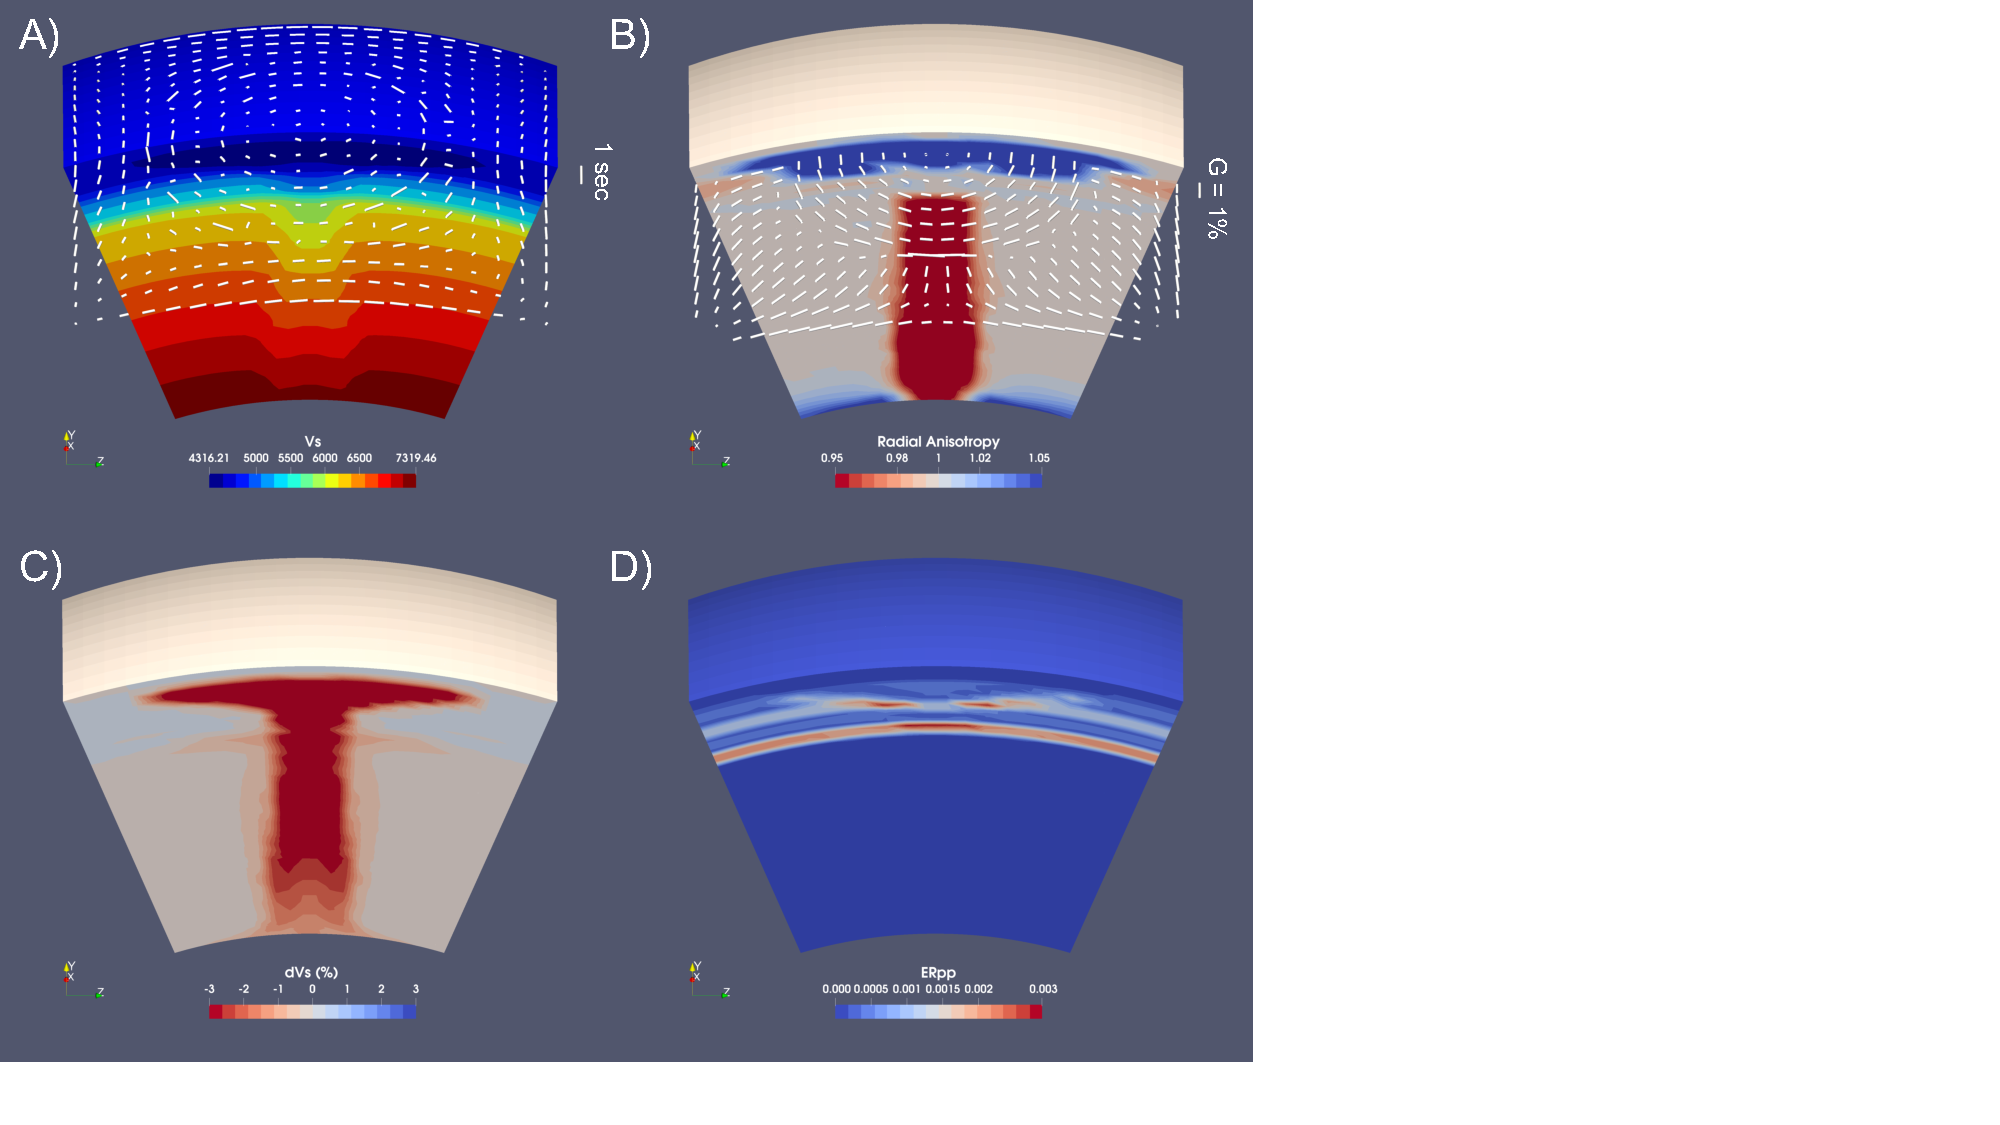
\includegraphics[width=1.0\textwidth]{VIZTOMO/plume.pdf}
    \caption{Example of a 3D thermo-mechanical model of an axi-symmetric thermal plume rising from the CMB in spherical coordinates. Only half of the eulerian grid generated with \viztomotitle{} is showed. A) S-wave isotropic velocity together with SKS splitting patterns at the surface (see chapter \ref{chapter:sks}); B) Radial anisotropy together with azimuthal anisotropy patterns (white bars) at 180 km depth; C) S-wave velocity anomalies (\%); D) Reflected P-P energy (note the lateral variations of the 410 and 660 km discontinuities as a function of the temperature anomaly).
    }
    \label{fig:plume}
\end{figure}

\begin{figure}[ht]
    \centering
    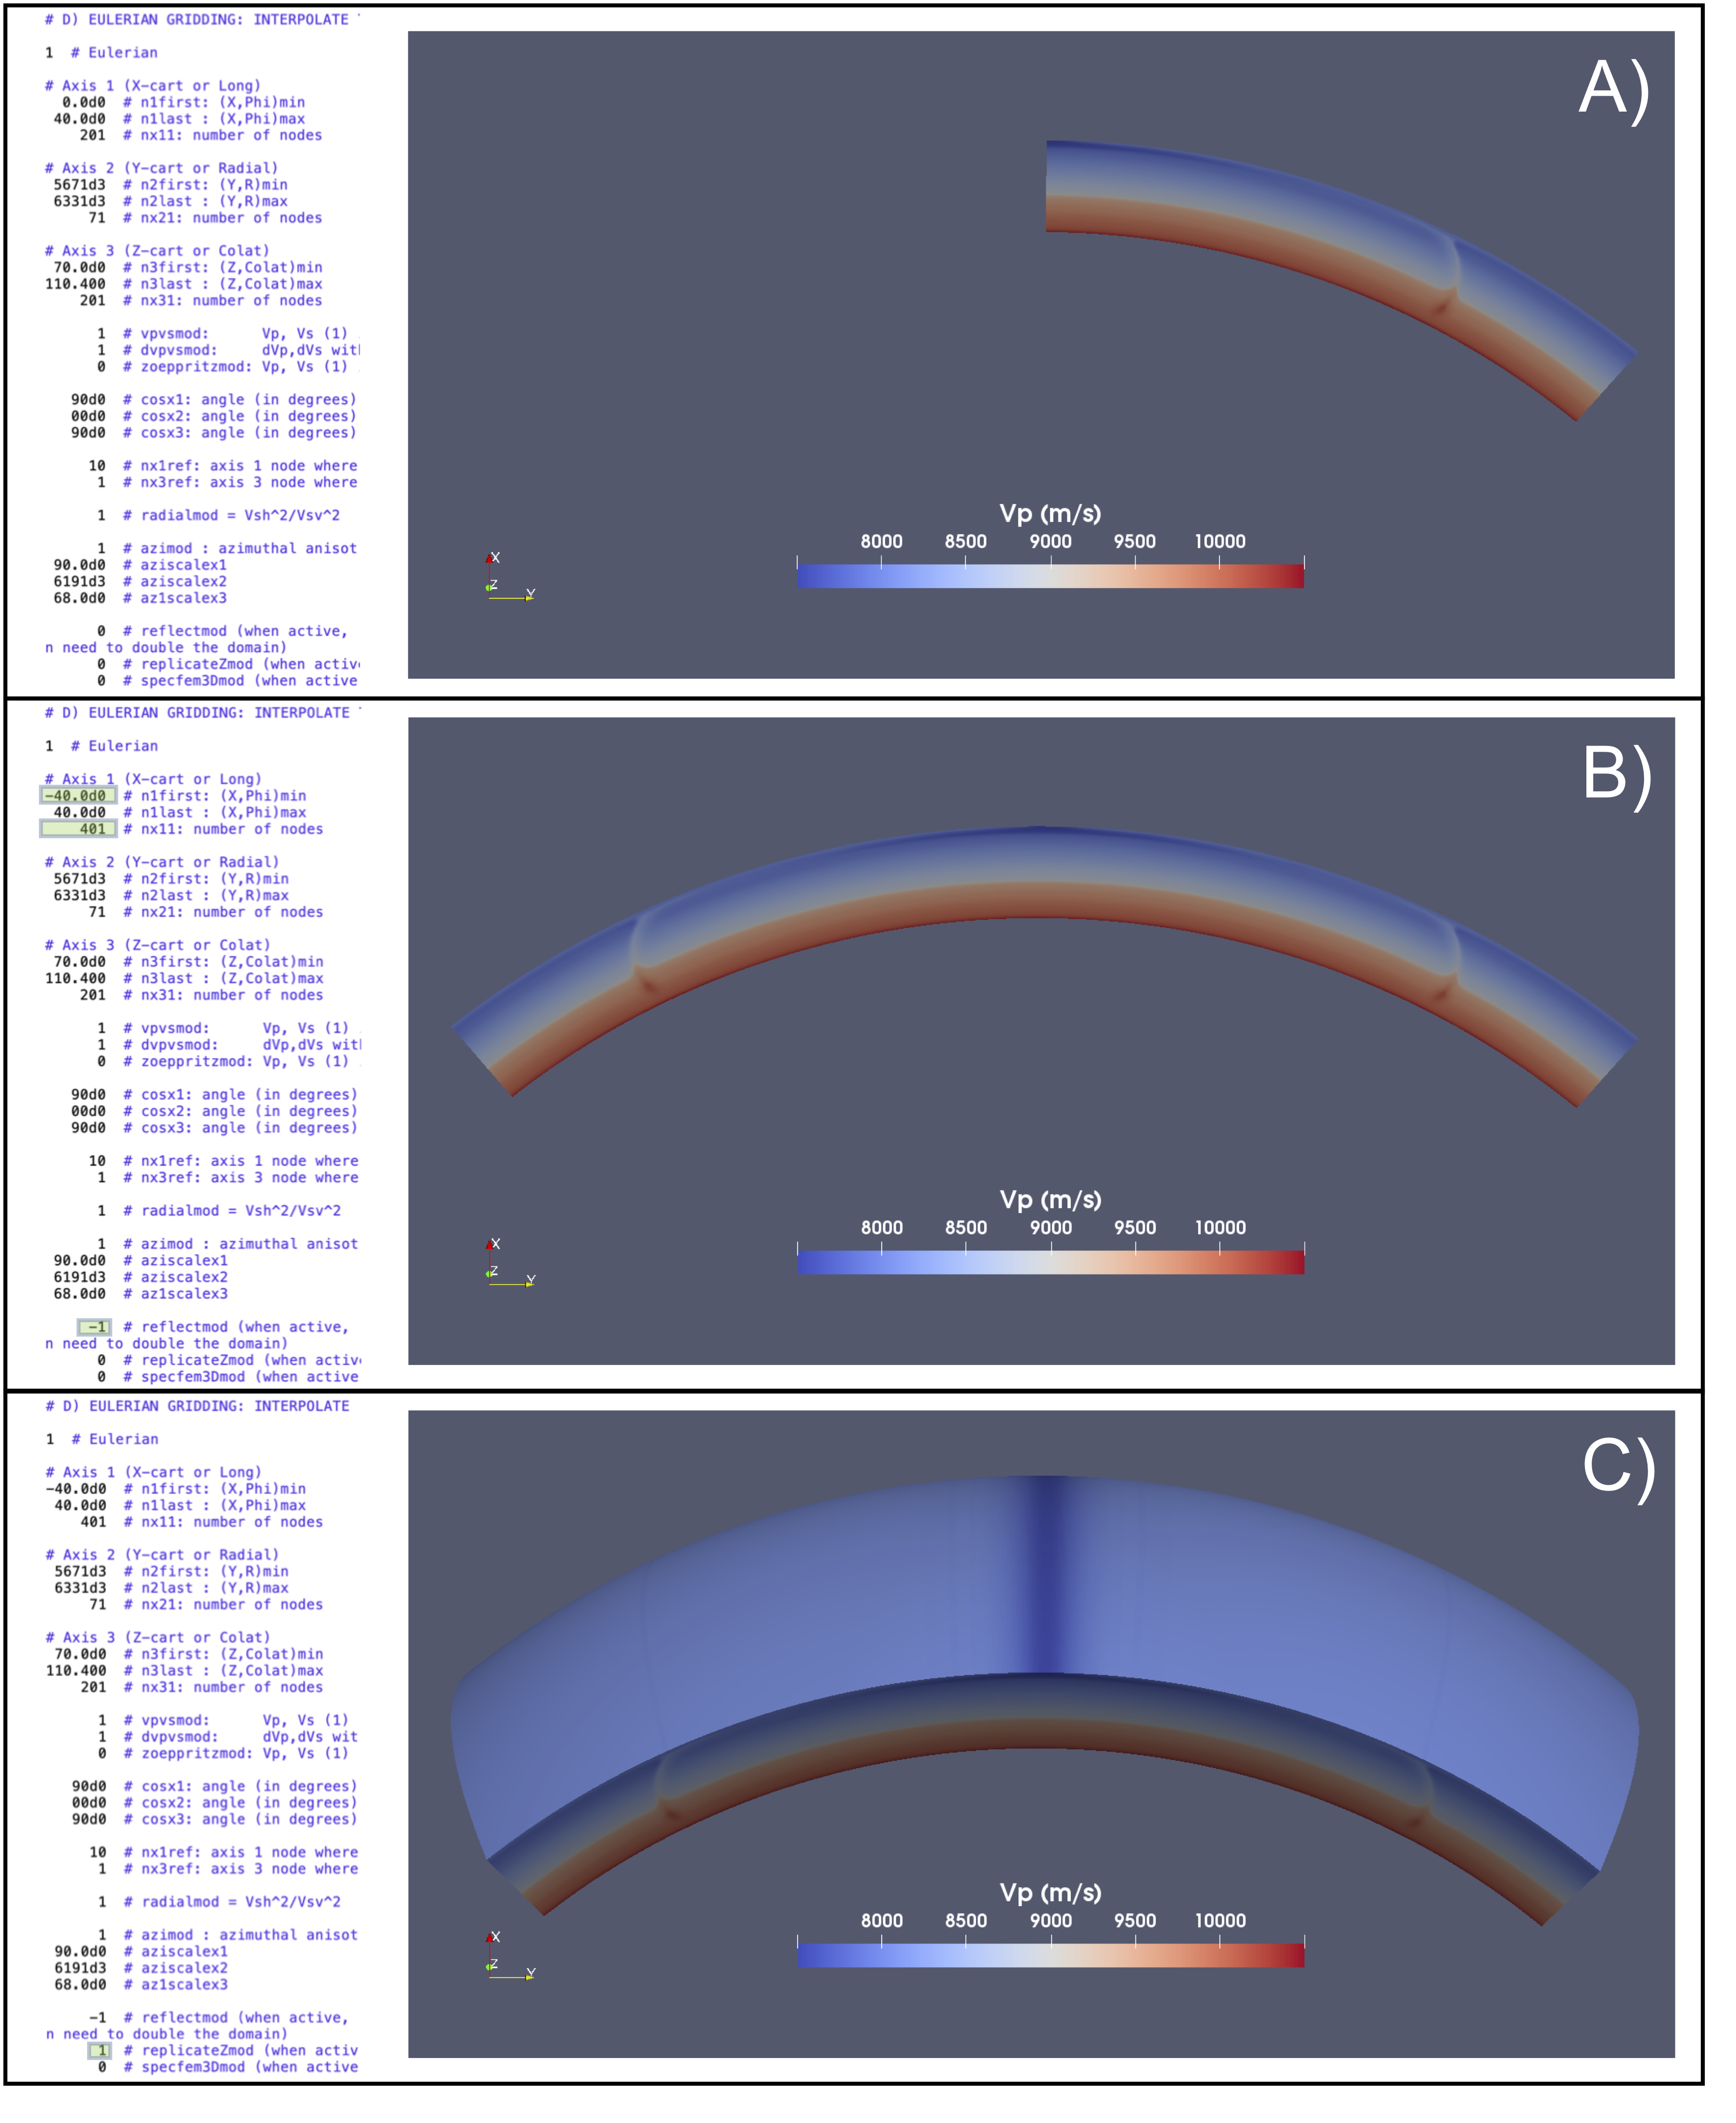
\includegraphics[width=1.0\textwidth]{VIZTOMO/reflectreplicate.png}
    \caption{Isotropic P-wave velocity of a 2D petrological-thermo-mechanical model of subduction in polar coordinates (see section \ref{section:cookbook_2Dsubduction}) (A). The same model reflected with respect to the oceanic ridge (B) and then replicated along the ridge axis (C). Right column: input variables in \texttt{viztomo\_input.dat}; the variations with respect to the configuration in the case right above is highlighted in pale green. Left column: P-wave velocity.  
    }
    \label{fig:reflectreplicate}
\end{figure}



%\vfill % Fill the rest of the page with whitespace


\section{SPECFEM3D simulations within the domain built with \viztomotitle{}}

To be finalized, coming soon!.\\

\vfill % Fill the rest of the page with whitespace
\chapter{\skstitle: synthetic SKS splitting}
\label{chapter:sks}

Synthetic SKS splitting is computed with routines included in FSTRACK (\citet{becker2006epsl}). An additional routine (savstack.f90) is provided to define a grid of seismic stations and, per each seismic station, build a stack of mantle horizontal layers by averaging elastic tensors and densities of crystal aggregates that are located close to the vertical projection of the station at depth and that are loaded from the \texttt{Cijkl*.h5} output file generated with \drexmtitle{} .\\*
\vspace{0.5cm}

\texttt{COMPILE:}\\*

\begin{itemize}
    \item Untar \texttt{fstrack.tar.gz: tar -zxvf fstrack.tar.gz}
    \item Execute the \texttt{Makefile} in \texttt{fstrack/single\_layer}\footnotemark:   \texttt{make}
    \item Execute the \texttt{Makefile} in \texttt{fstrack/multi\_layer}:   \texttt{make}
    \item copy the binary file \texttt{anicake} from \texttt{/fstrack/bin} directory to the \skstitle{} directory containing the bash file \texttt{pbs\_sks}. Directory \texttt{/fstrack} can be now deleted, if wanted.
    \item Execute \texttt{./bash\_compile} in \skstitle{}
\end{itemize}

\footnotetext{Depending on the Intel Fortran Compiler and environment settings, you need to add \texttt{F77=ifort},\texttt{F90=ifort},\texttt{CC=icc} to each of the two \texttt{Makefile}. This is done in the FSTRACK version present in this package}

\vspace{0.5cm}

\texttt{RUN:} submit the \texttt{pbs\_sks} bash file which consecutively runs:\\
\texttt{./stack\_calc args} (generates a stack of horizontal layers with different elastic tensors)\\
\texttt{mpiexec  -np nprocs  ./split\_calc args} (computes splitting paramters averaged over back-azimuth)\\
\\*

\section{Parameter input file(s)}
In \skstitle{}, open the bash file \texttt{pbs\_sks} and set the directory \fonts{cijkl\_dir} (String) where the \cijkltitle{} file that you want to process is and its filenumber \fonts{timestep} (4 digit Integer). Other parameters are rarely modified, and thus here not explained (but please feel free to contact the software developer for more infos). The number of processes (nprocs) is defined by the run control parameters (shown as an example in \texttt{pbs\_sks}). 
At first, the code \texttt{stack\_calc}, executed by one process, generate a 2D virtual grid of seismic stations and the underlying vertical stack of homogeneous elastic horizontal layers. Successively SKS splitting is computed by nprocs OpenMPI processes by executing \texttt{split\_calc} (modified after Thorsten Becker).

Set the following parameters in file \texttt{stack\_input.dat} (to be placed in the \fonts{cijkl\_dir} directory) to build the grid of virtual seismic stations (in 2D models, ignore \fonts{nsx3, i3first, i3last}):

\begin{itemize}
    \item \fonts{nsx1}: Integer. Number of seismic stations along horizontal axis 1 of the domain defined below
    \item \fonts{nsx3}: Integer. Number of seismic stations along horizontal axis 3 of the domain defined below
    \item \fonts{depthaxis}: Integer
    \begin{itemize}
	    \item[] \fonts{0}: vertical axis positive downward
        \item[] \fonts{1}: vertical axis positive upward
    \end{itemize}
\end{itemize}
    
Define the domain where to set the grid of seismic stations, and the volume enclosing the Lagrangian crystal aggregates sampled by the SKS waves. As SKS waves are mostly sensitive to anisotropy at upper mantle depths (\citet{sieminski2008bssa}), the vertical extent of the domain is usually that of the upper mantle.
\begin{itemize}
    \item \fonts{i1first}, \fonts{i1last}: seismic stations grid and Lagrangian domain axis 1: min, max coordinates (in unit length in cartesian coord.; in degrees in polar/spherical coord.).  
    \item \fonts{i2first}, \fonts{i2last}: Lagrangian domain axis 2: min, max coordinates (in unit length).  
    \item \fonts{i3first}, \fonts{i3last}: seismic stations grid and Lagrangian domain axis 3: min, max coordinates (in unit length in cartesian coord.; in degrees in spherical coord.).
    \item \fonts{maxdist}: maximum horizontal distance of mantle aggregates to be used for the interpolation of density and elastic tensor from the vertical projection at depth of the seismic station (in unit length). As the Fresnel zone of SKS waves is 100-200 km in the upper mantle, maxdist is tipically set to 50-100 km.
    \item \fonts{minlayer}: minimum thickness of each mantle layer (in unit length). This is to avoid a very slow computation resulting from the formation of too many horizontal mantle layers when Lagrangian aggregates are densely packed. The max. number of layers set in anicake.F is 500. 
    \item \fonts{Xscale}: scaling factor used to convert depth in km as Depth [km] = Depth [geodynamic model units] $\cdot$ \fonts{Xscale}. As an example, if depth is defined in meters in the geodynamic model, \fonts{Xscale} must be set equal to $10^{-3}$.  
\end{itemize}

\section{Compute SKS splitting}
By running \texttt{./calc\_split}, the seismic stations position and vertical stack of averaged elastic tensors scaled by density are saved in directory \fonts{cijkl\_dir}\texttt{/seismic\_stations}, while the apparent SKS splitting computed as a function of the back-azimuth every 5 degrees are saved in files \fonts{cijkl\_dir}\texttt{/splitting/split$*$.dat.gz}, where $*$ is the seismic station number. \\*
The azimuthally averaged fast azimuth and delay times, together with standard deviations and station position, are saved in \fonts{cijkl\_dir}\texttt{/splitting/split.0.$*$.staat}, where $*$ is the \cijkltitle{} file number.\\*

\section{SKS splitting visualization}
Files \texttt{split.0.$*$.staat} can be processed with file \texttt{/viz/read\_sks\_splitting.m}, by setting the input parameters. The script plots the SKS splitting averages for a quick view, and generates \texttt{$*$.xmf} and \texttt{$*$.h5} files for visualization in Paraview via the Glyph plot filter. In this way, the SKS data can be superimposed over the geodynamic model and/or the Eulerian grids generated with \viztomotitle{}   (Fig. \ref{fig:radial+sks}). 

Examples of \texttt{stack\_input.dat} and \texttt{read\_sks\_splitting.m} are available for each of the models shown the cookbooks chapter \ref{chapter:cookbooks}.

\begin{figure}
    \centering
    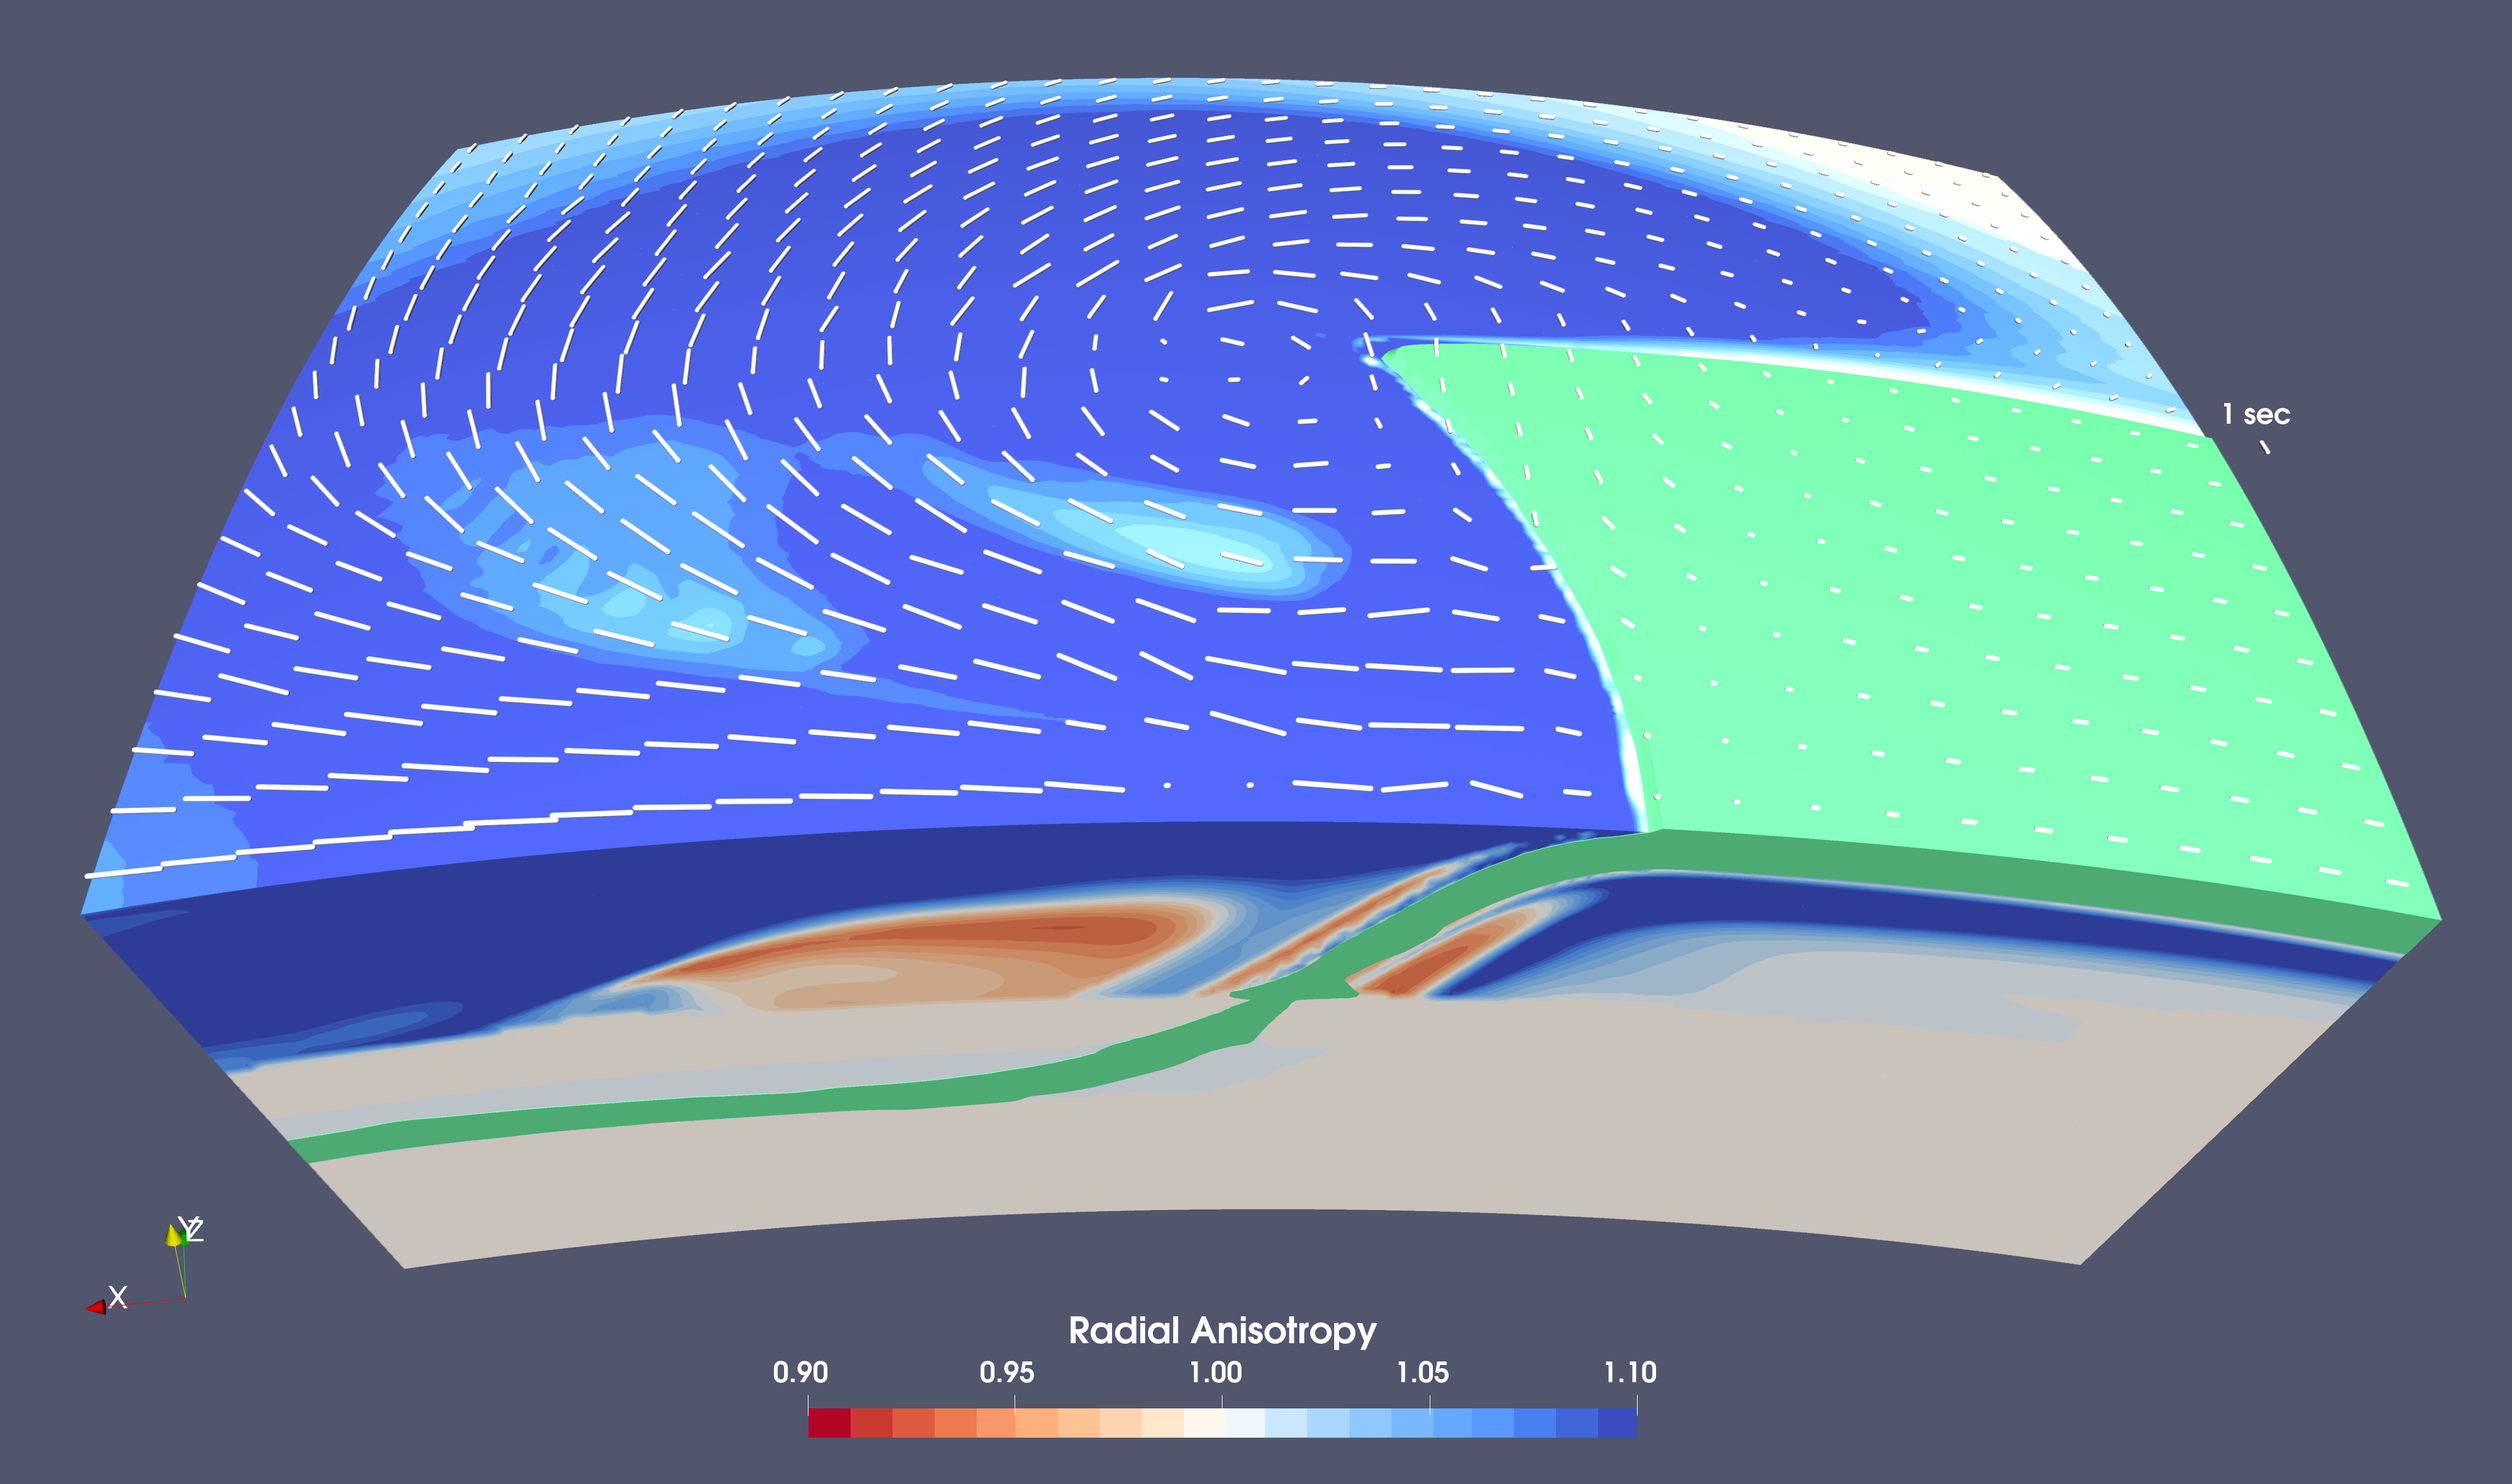
\includegraphics[width=1.0\textwidth]{SKS-SPLIT/Radial+SKS.png}
    \caption{Example of a 3D thermo-mechanical model of subduction in spherical coordinates. The front wall is the subduction zone mid-plane, and it is a symmetric boundary. The green surface enclose material with +1\% Vp anomalies which are related to the cold slab temperatures (note the thicker anomaly around the 410 km discontinuity, which is due to the upwelling of the $Ol \leftrightarrows Wd$ phase transition). The volume is color coded according to radial anisotropy and it has been generated with \viztomotitle{} after running \drexmtitle. The white bars are the mean SKS splitting for each of the seismic stations computed with the \skstitle{} software.}
    \label{fig:radial+sks}
\end{figure}




  



 

\chapter{\psitomotitle: Platform for Seismic Imaging (Deterministic)}
\label{chapter:psi_d}

\section{Overview} \label{PSI_D:Overview}
The Platform for Seismic Imaging (\psitomotitle{}) is a Julia package for performing forward and deterministic inverse modelling of seismic datasets. Another stochastic inversion methodology is under development and planned for a future release (see Del Piccolo et al., 2023). The primary motivation for its development was to facilitate the conversion of mantle geodynamic models into realistic seismic velocity models that may in turn be compared to imaging results from real arrays. This allows one to better understand how geodynamic features may be represented in seismic images and to identify potential artefacts--particularly those arising from neglecting anisotropy \citep[e.g.][]{bezada2016g3, vanderbeek2021, vanderbeek2023}. To this end, synthetic seismic datasets can be generated directly from elastic models produced via \viztomotitle{} (Chapter \ref{chapter:viztomo}) and subsequently inverted for both isotropic and/or anisotropic parameters. Note that only \viztomotitle{} models in spherical coordinates are supported at this time.

At present, \psitomotitle{} can predict P and S travel-times, splitting intensity, and shear wave splitting parameters in a ray-theoretical framework. Forward calculations are supported for models parameterized by (1) isotropic body wave velocities, (2) Thomsen parameters describing hexagonally anisotropic media, and (3) the full 21-component elastic tensor. Travel-time and splitting intensity datasets can be inverted for both isotropic and hexagonally anisotropic 3D models with arbitrary symmetry axis orientations. The inversion is performed using an iterative Gauss-Newton approach to solve for the model perturbations that minimize the sum of the squared data residuals in addition to constraints on the model norm and Laplacian. For a complete description of the methodology see \cite{vanderbeek2021} and \cite{vanderbeek2023}.


\section{Installation} \label{PSI_D:Installation}
\psitomotitle{}, may be installed from Julia's package manager,

\texttt{julia> using Pkg} \\
\texttt{julia> Pkg.add(url="https://github.com/bvanderbeek/PSI\_D.git")}

\textbf{Attention non-Windows users!} For travel-time and ray path calculations, \psitomotitle{} uses the \textbf{TauP Toolkit} [Crotwell et al., 1999]. For the Julia wrapper to this Java program to function properly, the environment variable \texttt{JULIA\_COPY\_STACKS = yes} must be defined. This may be done within the shell configuration file or in Julia prior to loading the \psitomotitle{} package,

\texttt{julia> ENV["JULIA\_COPY\_STACKS"] = "yes"}

\textbf{Attention Mac users!} To avoid Java related segmentation faults, Julia must be started with the flag \texttt{---handle-signals=no}. Note that this may cause multithreading in Julia to crash.

A pure Julia implementation of the travel-time calculations and ray tracing is planned for a future release to avoid these Java-related inconveniences.

\section{Forward Modelling} \label{PSI_D:Forward Modelling}

All the parameters required to make predictions are defined in a TOML file (see \path{https://toml.io/en/}). An example parameter file is located in: \path{examples/SinkingSlab/psi_input/psi_parameters_synthetic.toml}. The TOML table headings and variables are detailed below (\ref{forward_parameters}).

Once the parameter file is defined, predictions can be made by calling the forward problem function with the parameter file as input, e.g.,

\texttt{julia> psi\_forward("psi\_input/psi\_parameters\_synthetic.toml")}

Upon completion of the forward calculation, the predictions will be written to \texttt{csv}-formatted files in the output directory specified in the parameter file. A separate file is generated for each observation and phase (i.e., P or S) pair. The structure of these files is detailed below. A copy of the parameter file used to call \texttt{psi\_forward} will also be saved.

\subsection{Parameter file variables for forward modelling} \label{forward_parameters}
1. \texttt{[Output]}
\begin{itemize}
\item \texttt{output\_directory}: Path (String) to the directory where results are written.
\item \texttt{tf\_time\_stamp}: Flag (Boolean) that when \texttt{true} will write results to a time-stamped folder (\texttt{yymmdd\_hhmmss}) in \texttt{output\_directory}. This is for convenience if one does not want to define unique names for every run.
\end{itemize}
At least one of the following observations types should be defined,

2.1. \texttt{[Observations.TravelTime.CompressionalWave]}
\begin{itemize}
\item \texttt{filename}: Path (String) to file containing P-wave travel-time data. Data should be written to a \texttt{csv}-formatted file with the following columns, travel-time (s), error (s), dominant waveform period (s; this will be used in the future for finite-frequency kernels), IASPEI recognized phase name, source ID (Integer), receiver ID (String), Channel (String; not currently used for any calculations but for reference).
\end{itemize}
2.2. \texttt{[Observations.TravelTime.ShearWave]}
\begin{itemize}
\item \texttt{filename}: Defined as above. However, for anisotropic forward calculations an additional 8$^{\text{th}}$ column containing the polarization azimuth measured counter-clockwise positive from the Q-channel (in ray-aligned QTL-coordinates) should be defined. If not present, shear waves are assumed to be radially polarized.
\end{itemize}
2.3. \texttt{[Observations.SplittingIntensity.ShearWave]}
\begin{itemize}
\item \texttt{filename}: Defined as above for S-wave travel-times (replacing the travel-time and error columns with the splitting intensity values).
\end{itemize}
2.4. \texttt{[Observations.SplittingParameters.ShearWave]}
\begin{itemize}
\item \texttt{filename}: Defined similar to the S-wave travel-time file. However, the first two columns contain the split time (s) and fast-azimuth (radians), respectively. The 3$^{\text{rd}}$ and 4$^{\text{th}}$ columns contain the errors in the split time and fast-azimuth.
\end{itemize}

3.1 \texttt{[Model]}
\begin{itemize}
\item \texttt{parameterisation}: The type of parameterization (String) used to define the velocity model. Options are \texttt{"IsotropicVelocity"},\\ \texttt{"HexagonalVectoralVelocity"} for hexagonal anisotropic models with arbitrary symmetry axis orientations, or \texttt{"ElasticVoigt"} when models are defined using the 21-component elastic tensor.
\item \texttt{theModel}: Path (String) to the \texttt{csv}-file containing model data. At present, models must be defined on a regular grid in spherical coordinates. Each model file must contain 3 header lines,\\
Header 1: Earth radius (km), longitude of model origin (i.e. center; decimal degrees), latitude of model origin (i.e. center; decimal degrees), rotation of model from north (radians; for future use);\\
Header 2: Number of nodes in longitude, number of nodes in latitude, number of nodes in radial direction\\
Header 3: Half-arc width of model in east-west direction (degrees), half-arc width of model in north-south-direction, maximum depth of model (km).\\
For \texttt{IsotropicVelocity} models, the values are printed first by increasing longitude, then increasing latitude, and lastly decreasing elevation. Each data row contains the following columns, longitude (decimal degrees), latitude (decimal degrees), elevation (km), Vp (km/s), Vs (km/s).\\
For \texttt{HexagonalVectoralVelocity} models, an additional 4$^{\text{th}}$ header line containing a single Boolean is required specifying if the exact (1) or weak (0) form of Thomsen's phase velocity equations are used in the forward calculation. Data rows are printed as for \texttt{IsotropicVelocity} with columns 4-11 defining $\alpha$ (i.e. symmetry axis P-velocity; km/s), $\beta$ (i.e. symmetry axis P-velocity; km/s), $f$ the anisotropic fraction, $\phi$ the symmetry axis azimuth (radians), $\theta$ the symmetry axis elevation (radians), and the ratios between the anisotropic strength and the Thomsen parameters, $r_{\epsilon}$ = $\epsilon/f$, $r_{\eta}$ = $(\epsilon - \delta)/f$, and $r_{\gamma}$ = $\gamma/f$.\\
For \texttt{ElasticVoigt} models, an additional 4$^{\text{th}}$ header line containing a single Boolean is required specifying if the elastic constants are density-nomalized (1) or not (0). The 21 elastic coefficients should be written to columns 4-24 in the order, $c_{11}$, $c_{12}$,...,$c_{16}$, $c_{22}$, $c_{23}$,...,$c_{26}$,...,$c_{66}$. When density-normalized, the units should be m$^2$/s$^2$. If not density normalized, the 25$^{\text{th}}$-column should contain the density (kg/m$^3$) and the elastic coefficients given in GPa.
\end{itemize}

3.2 \texttt{[Model.Aquisition]}
\begin{itemize}
\item \texttt{source\_data}: Path (String) to \texttt{csv}-file with seismic source data. The data columns are organized as follows: numeric ID, longitude (decimal degrees), latitude (decimal degrees), elevation (km).
\item \texttt{receiver\_data}: Path (String) to \texttt{csv}-file with seismic receiver data. The file should be formatted the same as \texttt{source\_data} with the exception that the receiver ID will be interpreted as a string.
\end{itemize}

3.3 \texttt{[Model.Methods.TauP]}
\begin{itemize}
\item \texttt{reference\_model}: Name (String) of the reference 1D model used for computing ray paths with \textbf{TauP}. Any built-in \textbf{TauP} model names are valid (e.g., \texttt{"iasp91"}, \texttt{"ak135"}) and custom velocity profiles may also be used provided they comply with \textbf{TauP} format requirements.
\item \texttt{DL}: Ray path discretization interval (km). \textbf{TauP} ray paths are resampled at this level. An appropriate spacing is one that allows the details of the 3D velocity model to be accurately interpolated to the ray path.
\end{itemize}

\section{Inverse Modelling} \label{PSI_D:Inverse Modelling}

All the parameters required to run the inverse problem are defined in a TOML file similar to that used for the forward modelling (\ref{PSI_D:Forward Modelling}). An example parameter file for performing an inversion is located in: \path{examples/SinkingSlab/psi_input/psi_parameters_iso_inverse.toml}. The TOML table headings and variables are detailed below (\ref{inverse_parameters}).

Once the parameter file is defined, an inversion is run by calling the inverse problem function with the parameter file as input, e.g.,

\texttt{julia> psi\_inverse("psi\_input/psi\_parameters\_iso\_inverse.toml")}

Upon completion, a number of outputs will be generated and stored in the directory specified in the parameter file. These are described below in section \ref{inverse_output}.

\subsection{Parameter file variables for inverse modelling} \label{inverse_parameters}
All the forward modelling parameters detailed in \ref{forward_parameters} must also be defined in the inversion parameter file in addition to the following:

1. \texttt{[Model]}\\
If the starting model for the inversion is read from a file (as in the forward modelling) then no additional parameters are required under this TOML heading. \textbf{Note!} Only \texttt{IsotropicVelocity} and \texttt{HexagonalVectoralVelocity} parameterizations are allowed for inverse modelling. It's also possible to use the 1D TauP velocity profile as the starting model in which case the following additional definitions are required.
\begin{itemize}
\item \texttt{theModel}: This should be defined as an empty string (\texttt{""}) to trigger the use of the reference 1D TauP velocity model.
\end{itemize}

1.1. \texttt{[Model.Parameters]}\\
When using \texttt{HexagonalVectoralVelocity} default ratios between the Thomsen parameters ($\epsilon$, $\eta = \epsilon - \delta$, $\gamma$) and the anisotropic strength ($f$) must be defined.
\begin{itemize}
\item \texttt{ratio\_epsilon}: The ratio $\epsilon/f$.
\item \texttt{ratio\_eta}: The ratio $\eta/f$.
\item \texttt{ratio\_gamma}: The ratio $\gamma/f$.
\end{itemize}

1.2: \texttt{[Model.CoordinateSystem]}\\
Because the coordinate system parameters are no longer read from the model file header, they must be defined.
\begin{itemize}
\item \texttt{R\_0}: The reference Earth radius (km).
\item \texttt{Lon\_0}: Longitude origin (i.e. center) of model domain (decimal degrees).
\item \texttt{Lat\_0}: Latitude origin (i.e. center) of model domain (decimal degrees).
\item \texttt{Rot}: Rotation of model with respect to North (degrees). Rotated coordinate systems are not yet implemented and this value should remain '0'.
\end{itemize}

1.3. \texttt{[Model.Mesh]}\\
Define the size of the forward model domain.
\begin{itemize}
\item \texttt{DX\_1}: Longitudinal half-width of model domain (decimal degrees).
\item \texttt{DX\_2}: Latitudinal half-width of model domain (decimal degrees).
\item \texttt{DX\_3}: Maximum depth (positive) of model domain (km).
\item \texttt{NX\_1}: Number of nodes in the longitudinal direction.
\item \texttt{NX\_2}: Number of nodes in the latitudinal direction.
\item \texttt{NX\_3}: Number of nodes in depth.
\end{itemize}

2. \texttt{[Invert]}\\
All of the inversion parameters are defined under this heading in the TOML file. Excluding any of the parameters defined below from an inversion simply requires that it's not defined in the parameter file.

2.1. \texttt{[Invert.SourceStatics]}
Source statics can be defined for each observation type using a separate heading as shown below.

2.1.1. \texttt{[Invert.SourceStatics.TravelTime]}
Define the above heading in the TOML parameter file to invert for travel-time source static terms. A unique static for every source-observation type-phase tuple is included. Under this heading the following variables must be defined:
\begin{itemize}
\item \texttt{phases}: A vector of strings listing the phase types (\path{"CompressionalWave"} or \path{"ShearWave"}) to include.
\item \texttt{damping}: Vector of damping values that limit the norm of the static perturbations for each phase.
\item \texttt{tf\_jump}: Vector of booleans to minimise the cumulative (true) or incremental (false) static perturbation for each phase.
\end{itemize}

These variables can be repeated under \texttt{[Invert.SourceStatics.SplittingIntensity]} to include splitting intensity source statics. 


2.2. \texttt{[Invert.ReceiverStatics]}\\
Receiver statics are implemented in the same way as the source statics with the same variables defined under the headings \texttt{[Invert.ReceiverStatics.ObservationType]} where \texttt{ObservationType} is a place-holder for \texttt{TravelTime} or \texttt{SplittingIntensity}.

2.3. \texttt{[Invert.Velocity]}\\
Under the \texttt{Velocity} sub-heading are defined isotropic and anisotropic seismic velocity inversion parameters.

2.3.1. \texttt{[Invert.Velocity.Isotropic]}
\begin{itemize}
\item \texttt{parameterisation}: Here we define the type of parameterization to use for the isotropic velocity fields. Currently, the only option is "InverseIsotropicSlowness". In the future, one may want to invert directly for velocity (rather than slowness) or relative velocity perturbations (i.e. dlnV).
\item \texttt{coupling\_option}: This parameter is for future use in joint P and S velocity inversions. It will describe how to couple P and S velocity perturbations. The only option currently implemented is '0' which does not enforce any coupling between P and S velocity perturbations.
\end{itemize}

2.3.1.1. \texttt{[Invert.Velocity.Isotropic.Mesh]}\\
Define the grid on which the isotropic inversion parameters are discretized. The inversion grid is separate from the forward model grid such that we can choose to solve for heterogeneity on a different scale than the starting model. This is useful when the starting model contains \textit{a priori} fine-scale structure (e.g., sediment basins). The variables for this field are the same as those described under \texttt{[Model.Mesh]} (i.e. \path{type}, \path{DX_1}, \path{DX_2}, \path{DX_3}, \path{NX_1}, \path{NX_2}, \path{NX_3}).

2.3.1.2. \texttt{[Invert.Velocity.Isotropic.P]}\\
Define the regularization parameters for P-velocity perturbations. If this heading is not defined, will not invert for P-velocity perturbations.
\begin{itemize}
    \item \texttt{damping\_weight}: Damping value that limits the norm of the velocity perturbations.
    \item \texttt{tf\_min\_cumulative}: Boolean to minimise cumulative (true) or incremental (false) norm of the of velocity perturbations.
    \item \texttt{smoothing\_weights}: Smoothing weights to enforce spatially smooth velocity perturbations in x1-, x2-, and x3-directions.
    \item \texttt{tf\_smooth\_cumulative}: Boolean to minimise cumulative (true) or incremental (false) Laplacian of the velocity perturbations with respect to the starting model.
\end{itemize}

2.3.1.3. \texttt{[Invert.Velocity.Isotropic.S]}\\
Define the regularization parameters for S-velocity perturbations. If this heading is not defined, will not invert for S-velocity perturbations. Variables for this section are the same as those detailed in \path{[Invert.Velocity.Isotropic.P]}.

2.4. \texttt{[Invert.Velocity.Anisotropic]}
Under this heading are the variables relevant to anisotropic inversions.

2.4.1. \texttt{[Invert.Velocity.Anisotropic.Mesh]}\\
Define the grid on which the isotropic inversion parameters are discretized. This is done as described under \texttt{[Invert.Velocity.Isotropic.Mesh]}.

2.4.1.1. \texttt{[Invert.Velocity.Anisotropic.Orientations]}\\
Define the regularization parameters for hexagonal symmetry axis inversions. If this heading is not defined, will not solve for any anisotropic parameters.
\begin{itemize}
    \item \texttt{parameterisation}: Here we define the type of parameterization to use for the isotropic velocity fields. Currently, the only option is \texttt{"InverseAzRadVector"} which will solve for the azimuthal and radial (i.e. vertical) components of the hexagonaly symmetry axis. The magnitude of the symmetry axis is directly proportional the P- and S-anisotropic fractions via the \texttt{ratio\_epsilon}, \texttt{ratio\_eta}, and \texttt{ratio\_gamma} forward model parameters.
    \item \texttt{damping\_weight}: Damping value that limits the norm of the anisotropy perturbations.
    \item \texttt{tf\_min\_cumulative}: Boolean to minimise cumulative (true) or incremental (false) norm of the of anisotropy perturbations.
    \item \texttt{smoothing\_weights}: Smoothing weights to enforce spatially smooth anisotropy perturbations in x1-, x2-, and x3-directions.
    \item \texttt{tf\_smooth\_cumulative}: Boolean to minimise cumulative (true) or incremental (false) Laplacian of the anisotropy perturbations with respect to the starting model.
\end{itemize}

3. \texttt{[Solver]}
\begin{itemize}
    \item \texttt{type}: Type of solver for performing the inverse problem. Only the LSQR-based method \texttt{"SolverLSQR"} is implemented. L-BFGS and gradient descent methods planed for future releases.
    \item \texttt{atol}: Stopping tolerance for LSQR algorithm (see lsqr documentation from IterativeSolvers.jl package). Default is \texttt{1.0e-6}.
    \item \texttt{conlim}: Convergence tolerance for LSQR algorithm (see lsqr documentation from IterativeSolvers.jl package). Default is \texttt{1.0e8}.
    \item \texttt{maxiter}: Maximum number of LSQR iterations allowed.
    \item \texttt{tf\_jac\_scale}: Boolean that if true, applies Levenberg-Marquardt style scaling of the regularization constraints. It is recommended that this parameter is true for most inversions.
    \item \texttt{nonliniter}: Maximum number of non-linear iterations (i.e. forward calculations and LSQR calls). Non-linear anisotropic inversions typically converge within 6 iterations. Iterations may stop before this criteria if the reduction in the sum of the squared residuals with respect to the prior iteration does not decrease significantly (as determined by an F-test at the 95\% confidence level).
\end{itemize}


\subsection{Inversion Output} \label{inverse_output}
When an inversion is run via\\
\texttt{julia> psi\_inverse("psi\_parameters.toml")}\\
the following outputs are generated:

\begin{itemize}
\item \texttt{FinalModel.vts}: VTK file that can be visualized in \textbf{Paraview}. This file contains both the starting model and the solution from the last iteration.
\item \texttt{RSJS\_ParameterField.vts}: VTK file that can be visualized in \textbf{Paraview}. This file contains the row-sum of the squared Jacobian elements (i.e. the squared derivative weight sum) and illustrates the data coverage for a given parameter field.
\item \texttt{chi\_squared.txt}: This file summarizes the data fit at each iteration. The first line of the file contains the critical F-value at which point iterations are stopped. The following lines list the iteration number and the corresponding F test statistic.
\item \texttt{RES\_ObservationType\_PhaseType.dat}: Data (\texttt{csv}) files containing the  residuals for each observation computed through the final iteration model. Separate files are generated for each observation type-phase pair. Files are formatted as described in \ref{forward_parameters} with the first column containing the residual (instead of the observed value).
\item \texttt{Parameters.dat}: A \texttt{csv} file containing the final model data in a format that can be used as a starting model for subsequent inversions (format is described in \ref{forward_parameters} under \texttt{[Model]}.
\item \texttt{Statics\_Sources.dat}: A \texttt{csv} file containing the final source statics. The columns are organized as follows, (1) source ID, Observation Type, Phase Type, static value.
\item \texttt{Statics\_Receivers.dat}: A \texttt{csv} file containing the final receiver statics. The columns are organized as follows, (1) receiver ID, Observation Type, Phase Type, static value.
\item \texttt{psi\_parameters.toml}: A copy of the parameter file used to run the inversion.
\end{itemize}


\section{Examples} \label{PSI_D:Examples}
Best way to get started using \psitomotitle{} is by looking through the examples. Two examples are included in the package repository and described below.

\subsection{Sinking Slab}
This example demonstrates how to generate a synthetic tomography model from a fully anisotropic elastic geodynamic model generated via \viztomotitle{}. The target model is a sinking slab generated by the Cookbook example \ref{section:cookbook_3Dspherical_sinking} and is located in the \psitomotitle{} repository under \path{examples/SinkingSlab}.

The \path{SinkingSlab} example include the following directories and files:

\texttt{jl-files/} Contains \textbf{Julia} scripts for generating synthetic data and running \psitomotitle{}
\begin{itemize}
    \item \texttt{mk\_inputs.jl}: Create synthetic array of seismic receivers and teleseismic sources for tomography.
    \item \texttt{mk\_synthetics.jl}: Runs the forward calculation (\path{psi_forward}) to generate synthetic observation files.
    \item \texttt{run\_inversion.jl}: Runs the inverse problem (\path{psi_inverse}).
    \item \texttt{example\_SKS\_SplittingParameters.jl}: Provides a short tutorial on how to generate SKS splitting parameters.
\end{itemize}

\texttt{psi\_input/} Contains input data for \psitomotitle{}.
\begin{itemize}
    \item \texttt{psitomo0020.dat}: The \viztomotitle{} elastic model used for creating synthetic observations.
    \item \texttt{ak135\_no\_crust.tvel}: A modified version (no crustal velocities) of the AK135 1D reference earth used as a starting model for the inversions.
    \item \texttt{psi\_parameters\_synthetic.toml}: The \psitomotitle{} parameter file referenced in \path{mk_synthetics.jl} to call \path{psi_forward} and generate synthetic data.
    \item \texttt{psi\_parameters\_iso\_inverse.toml}: The \psitomotitle{} parameter file for running isotropic inversion via \path{run_inversion.jl}.
    \item \texttt{psi\_parameters\_ani\_inverse.toml}: The \psitomotitle{} parameter file for running an anisotropic inversion via \path{run_inversion.jl}.
\end{itemize}

\texttt{psi\_output/} The location where the example will write inversion results.

\texttt{visualization/} Contains state-files that can be loaded to \textbf{Paraview} to automatically generate 3D plots of the isotropic (\path{render_solution_ISO_TTP.pvsm}) and anisotropic (\path{render_solution_ANI_TTP_TTS_SI.pvsm}) inversion results. Screen shots of the isotropic and anisotropic inversion results and predicted SKS split are provided in \path{figures}.


Here are the steps to reproduce the SinkingSlab synthetic tomography results:
\begin{enumerate}
    \item Build required input data. \viztomotitle{} generates a target model (\path{psi_input/psitomo0020.dat}) but we must define the seismic array and source distribution used in the tomographic reconstruction. These data are generated by running the \path{jl-files/mk_inputs.jl}. This script will create \path{psi_input/Sources.dat} and \path{psi_input/Receivers.dat} files and the place-holder observation files \path{psi_input/DUMMY_TravelTime_CompressionalWave.dat}, \path{psi_input/DUMMY_TravelTime_ShearWave.dat}, and \path{psi_input/DUMMY_SplittingIntensity_ShearWave.dat} (these contain P and S travel-times and S splitting intensity observation files for every source-receiver pair). The synthetic array consists of a regular grid of 625 receivers extending $\pm$10° in longitude and $\pm$10° in latitude. In total, 24 teleseismic sources are used for imaging; 12 at a range of 50° and 12 at 80° from the model center and equally distributed in back-azimuth.
    
    \item Generate synthetic observations. Using the inputs generated in step 1, we create synthetic travel-time and splitting intensity datasets by running \path{jl-files/mk_synthetics.jl}. This will create an output directory \path{psi_output/SYN_SinkingBlock} with the synthetic data files. This takes approx. 6 minutes to complete.
    
    \item Perform an isotropic inversion of the P-wave travel-times. Open \path{jl-files/run_inversion.jl} and set the variable \path{the_parameter_file} to \path{"psi_parameters_iso_inverse.toml"}. Then run the \textbf{Julia} script. The isotropic tomography results will be output in \path{psi_output/ISO_TTP}. This inversion completes in approx. 2 minutes.

    \item Perform an anisotropic inversion of P and S travel-times and S splitting intensity data. Repeat step 3 but first redefine \path{the_parameter_file} to \path{"psi_parameters_ani_inverse.toml"}. The anisotropic tomography results will be output in \path{psi_output/ANI_TTP_TTS_SI}. This inversion completes in approx. 18 minutes.
    
    \item Visualize the results. The inversion will generate vtk-files that may be visualized using \textbf{Paraview}. From \textbf{Paraview}, one can load the state-files \path{render_solution_ISO_TTP.pvsm} or \path{render_solution_ANI_TTP_TTS_SI.pvsm} to automatically generate some 3D plots of the isotropic and anisotropic inversions, respectively. However, upon loading the state file, one should select "Search files under a specified directory" in the dialog box and then specify the path the appropriate output folder in \path{psi_output/}. The expected results of the isotropic and anisotropic inversions are shown in Fig. \ref{fig:psi_d_results}.
\end{enumerate}

\begin{figure}[ht]
    \centering
    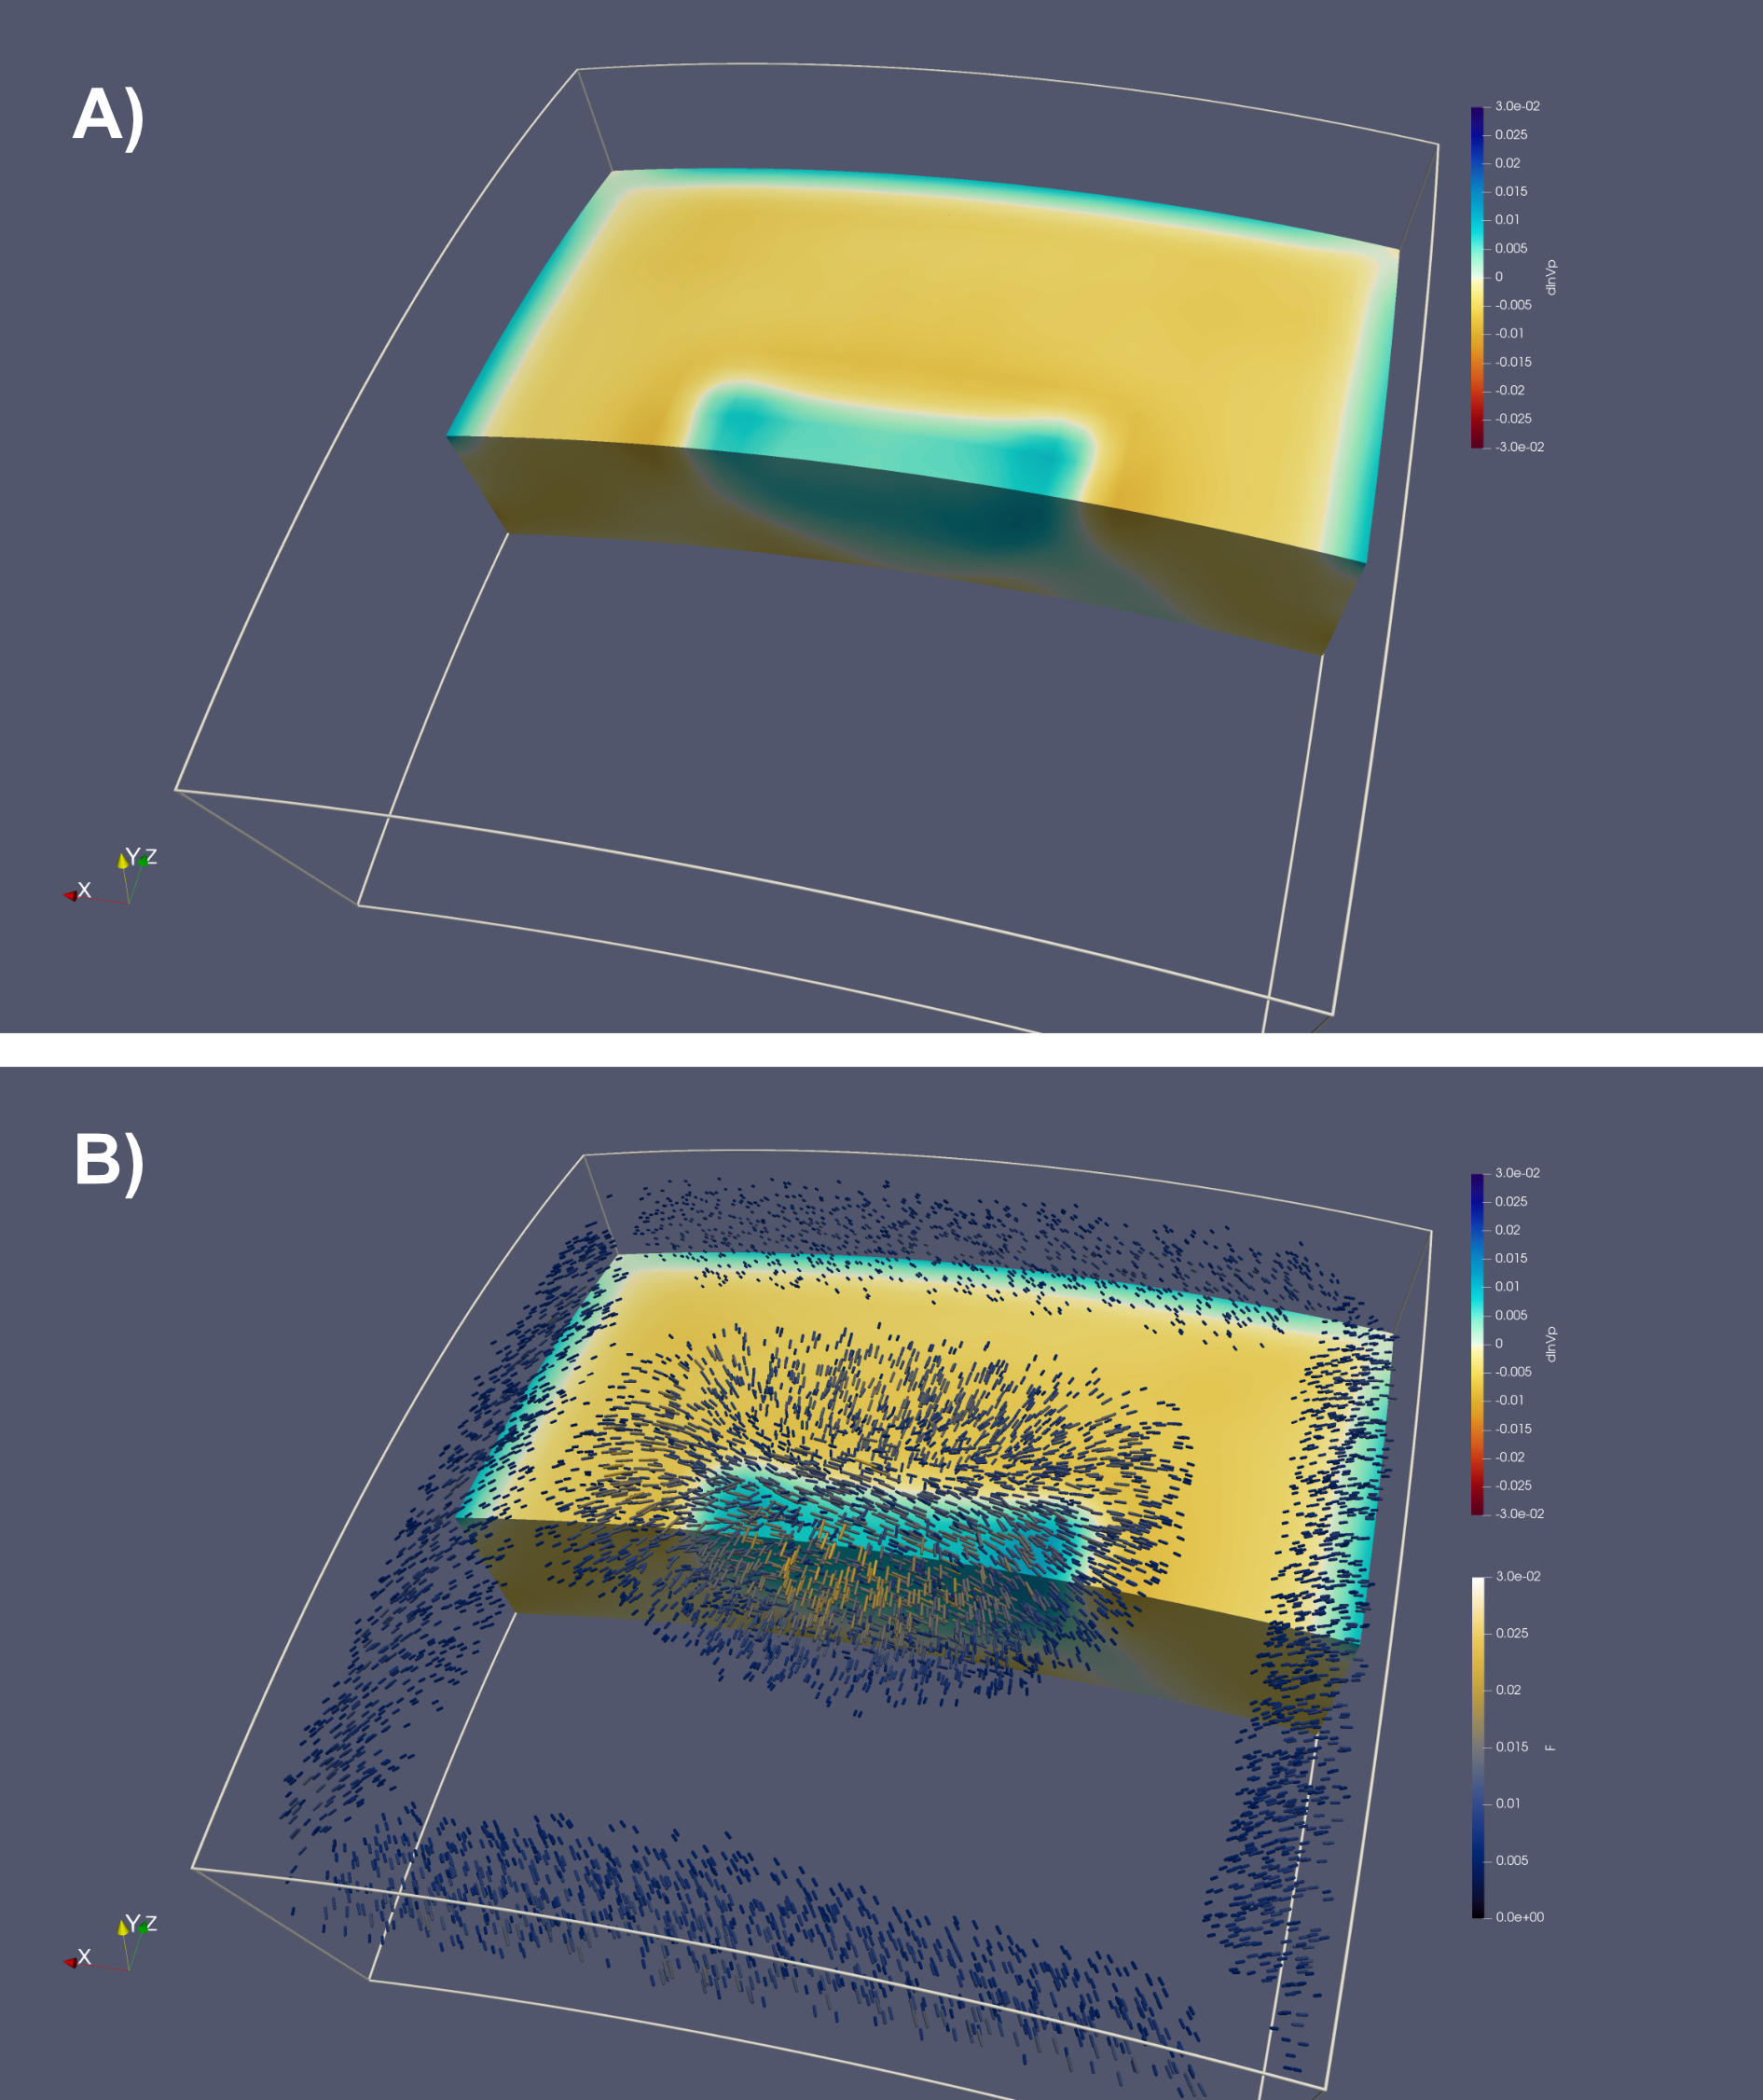
\includegraphics{PSI_D/PSI_D_Results.png}
    \caption{Sinking Slab tomography example. A) Isotropic inversion of P-wave travel-times. B) Anisotropic inversion of P and S travel-times and S splitting intensity. In both panels, the recovered isotropic P-wave anomaly is contoured and the model is sliced through the center of the sinking slab at 300 km depth and in the east-west direction; full extent of the model is outlined. In B), a random distribution of recovered hexagonal symmetry axes (i.e. fast axes) are plotted and colored by the anisotropic strength. Symmetry axes are shown only where the anisotropic strength is >0.5\%.\\
    }
    \label{fig:psi_d_results}
\end{figure}

\subsection{Subducting Plate}
In addition to the Sinking Slab example, we also include the files required to reproduce the anisotropic tomography results for the subducting plate shown in Figure \ref{fig:radial+sks} (or Figure 9 of the \textbf{ECOMAN} publication) and reproduced below in Fig. \ref{fig:psi_d_subduction}. The inputs required to run the inversion are located in \path{examples/SubductingPlate}. The reference \viztomotitle{} model file is not included due to its large size. To run the inversion, do \texttt{julia jl-files/run\_inversion.jl}. The results will be stored in \path{psi_output/ANI_TTP_TTS}. This inversion should finish in approx. 15 minutes. Once finished, load the state-file \path{visualization/render_model.pvsm} in \textbf{Paraview} (be sure to update the path to the appropriate output directory when prompted by the \textbf{Paraview} dialog box) and the tomographic results should appear as show in Fig. \ref{fig:psi_d_subduction}.

\begin{figure}[ht]
    \centering
    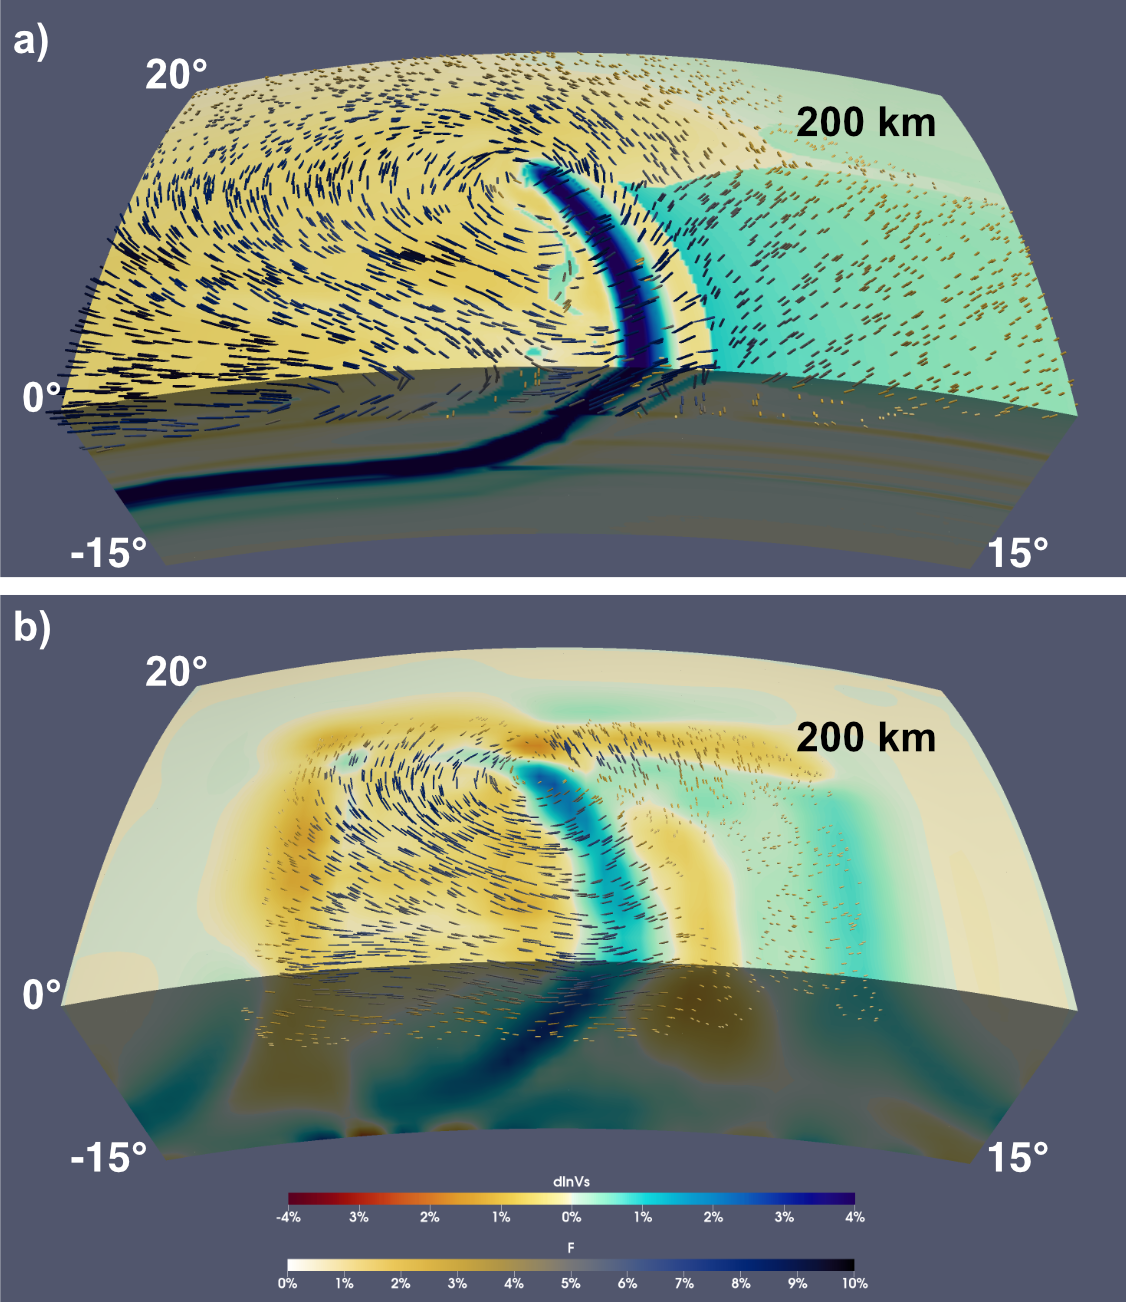
\includegraphics{PSI_D/PSI_D_Subduction.png}
    \caption{Synthetic subducting plate example. (a) Target anisotropic model generated from VIZTOMO. (b) Recovered anisotropic model obtained by inverting synthetic teleseismic P and S (relative) travel times computed from the model in (a). In both panels, the isotropic S-wave velocity perturbations are computed with respect to the far-field 1D velocity profile. Quivers parallel the hexagonal symmetry axis and are scaled and coloured by the anisotropic strength. The top surface shown is located at 200 km depth while the full model extends from 0-1000 km along the radial direction, 85°-115° along longitude, and 0-20° along latitude.\\
    }
    \label{fig:psi_d_subduction}
\end{figure}


% REFERENCES
% Aki, K., Christoffersson, A., \& Husebye, E. S. (1977). Determination of the three‐dimensional seismic structure of the lithosphere. Journal of Geophysical Research, 82(2), 277-296.

% Bezada, M. J., Faccenda, M., \& Toomey, D. R. (2016). Representing anisotropic subduction zones with isotropic velocity models: A characterization of the problem and some steps on a possible path forward. Geochemistry, Geophysics, Geosystems, 17(8), 3164-3189.

% Bodmer et al. (2020)

% Lévêque, J. J., \& Masson, F. (1999). From ACH tomographic models to absolute velocity models. Geophysical Journal International, 137(3), 621-629.

% Masson, Y., \& Romanowicz, B. (2017). Box tomography: localized imaging of remote targets buried in an unknown medium, a step forward for understanding key structures in the deep Earth. Geophysical Journal International, 211(1), 141-163.

% Munzarová, H., Plomerová, J., \& Kissling, E. (2018a). Novel anisotropic teleseismic body-wave tomography code AniTomo to illuminate heterogeneous anisotropic upper mantle: Part I—Theory and inversion tuning with realistic synthetic data. Geophysical Journal International, 215(1), 524-545.

% Paige, C. C., \& Saunders, M. A. (1982). LSQR: An algorithm for sparse linear equations and sparse least squares. ACM Transactions on Mathematical Software (TOMS), 8(1), 43-71.

% Schmandt, B., \& Humphreys, E. (2010). Seismic heterogeneity and small‐scale convection in the southern California upper mantle. Geochemistry, Geophysics, Geosystems, 11(5).

% Toomey, D. R., \& Foulger, G. R. (1989). Tomographic inversion of local earthquake data from the Hengill‐Grensdalur central volcano complex, Iceland. Journal of Geophysical Research: Solid Earth, 94(B12), 17497-17510.

% Toomey, D. R., Solomon, S. C., \& Purdy, G. M. (1994). Tomographic imaging of the shallow crustal structure of the East Pacific Rise at 9$^{\circ}$30′ N. Journal of Geophysical Research: Solid Earth, 99(B12), 24135-24157.

% VanderBeek \& Faccenda (in review)
\chapter{\cookbookstitle: some useful examples}
\label{chapter:cookbooks}

The following cookbooks are provided as examples to facilitate the user configuring  \drexmtitle{}, \viztomotitle{} and \skstitle{} runs in different geodynamic model domains. The input parameter files (\texttt{*\_input.dat}) should be structured as provided, that is, preserving the same sequence of parameters. However, not all the parameters need to be considered, as some of them are only used when required (i.e., in 2D, the 3rd dimension is ignored; the size of the domain where to set a fossil fabric is considered only when \fonts{fossifabric} is > 0; visualization of the Lagrangian and Eulerian fields is active only when \fonts{Lagrangian} and \fonts{Eulerian} are > 0, respectively; etc.).\\  
In order to minimize the size of the \vtptitle{} files required to compute mantle fabrics, the examples below have been generated by low- to medium-resolution geodynamic models, and, in several cases, where the flow fields have reached or are assumed to have reached steady-state conditions.
For each cookbook, we provide parameter input files for software \drexmtitle{}, \viztomotitle{}, \vizvisctitle{} and \skstitle{}. \\
From each of the software directory execute:\\  

\drexmtitle{}: \texttt{./drexm ../cookbooks/DIRECTORY/drexm\_input.dat}

\viztomotitle{}: \texttt{./viztomo ../cookbooks/DIRECTORY/viztomo\_input.dat}

\vizvisctitle{}: \texttt{./vizvisc ../cookbooks/DIRECTORY/vizvisc\_input.dat} (provided only for \texttt{/2Dpolar\_convection})

\skstitle{}: \texttt{./calc\_split\_from\_flow\_model}\footnotemark


\footnotetext{Open the bash file \texttt{pbs\_sks}, and at lines 20 and 22 set, respectively, the directory \fonts{cijkl\_dir} (String) where the \cijkltitle{} file that you want to process is (and where the \texttt{stack\_input.dat} file has been copied), and its filenumber \fonts{timestep} (4 digit Integer)}

\vfill  % Fill the rest of the page with whitespace

\section{Steady-state convection in 2D cartesian coordinates}
\label{section:cookbook_2Dcartesianconvection}

\texttt{DIRECTORY: /2Dcartesian\_convection}

A 2D incompressible flow field in cartesian coordinates is given by the following analytical solution, whereby the radial and tangential velocities are: \\
\begin{center}
    $V_x(x,y) = -V_{x0}\sin(k_x2\pi/W)\cos(k_y\pi/H)$ \\
    $V_y(x,y) =  V_{y0}\cos(k_x2\pi/W)\sin(k_y\pi/H)$ \\
\end{center}

where $x$ and $y$ are the horizontal and vertical distance, $V_{x0}$ and $V_{y0}$ a constants, $k_x$ and $k_y$ are the horizontal and vertical wave numbers, $W$ and $H$ are the domain width and height. 

The \fonts{V} field is computed with the \matlabtitle{} script \texttt{cartesiancells.m} and saved to \texttt{vtp0001.h5} as a function of the numerical resolution, horizontal and vertical wave numbers. The model is mechanical, and thus  \fonts{ptmod = 0} in \texttt{drexm\_input.dat}.
The mantle fabrics computed with \drexmtitle{} in steady-state conditions for 5 Myr and visualized with \viztomotitle{} are shown in Fig. \ref{fig:cartesiancells}.


\begin{figure}[ht]
    \centering
    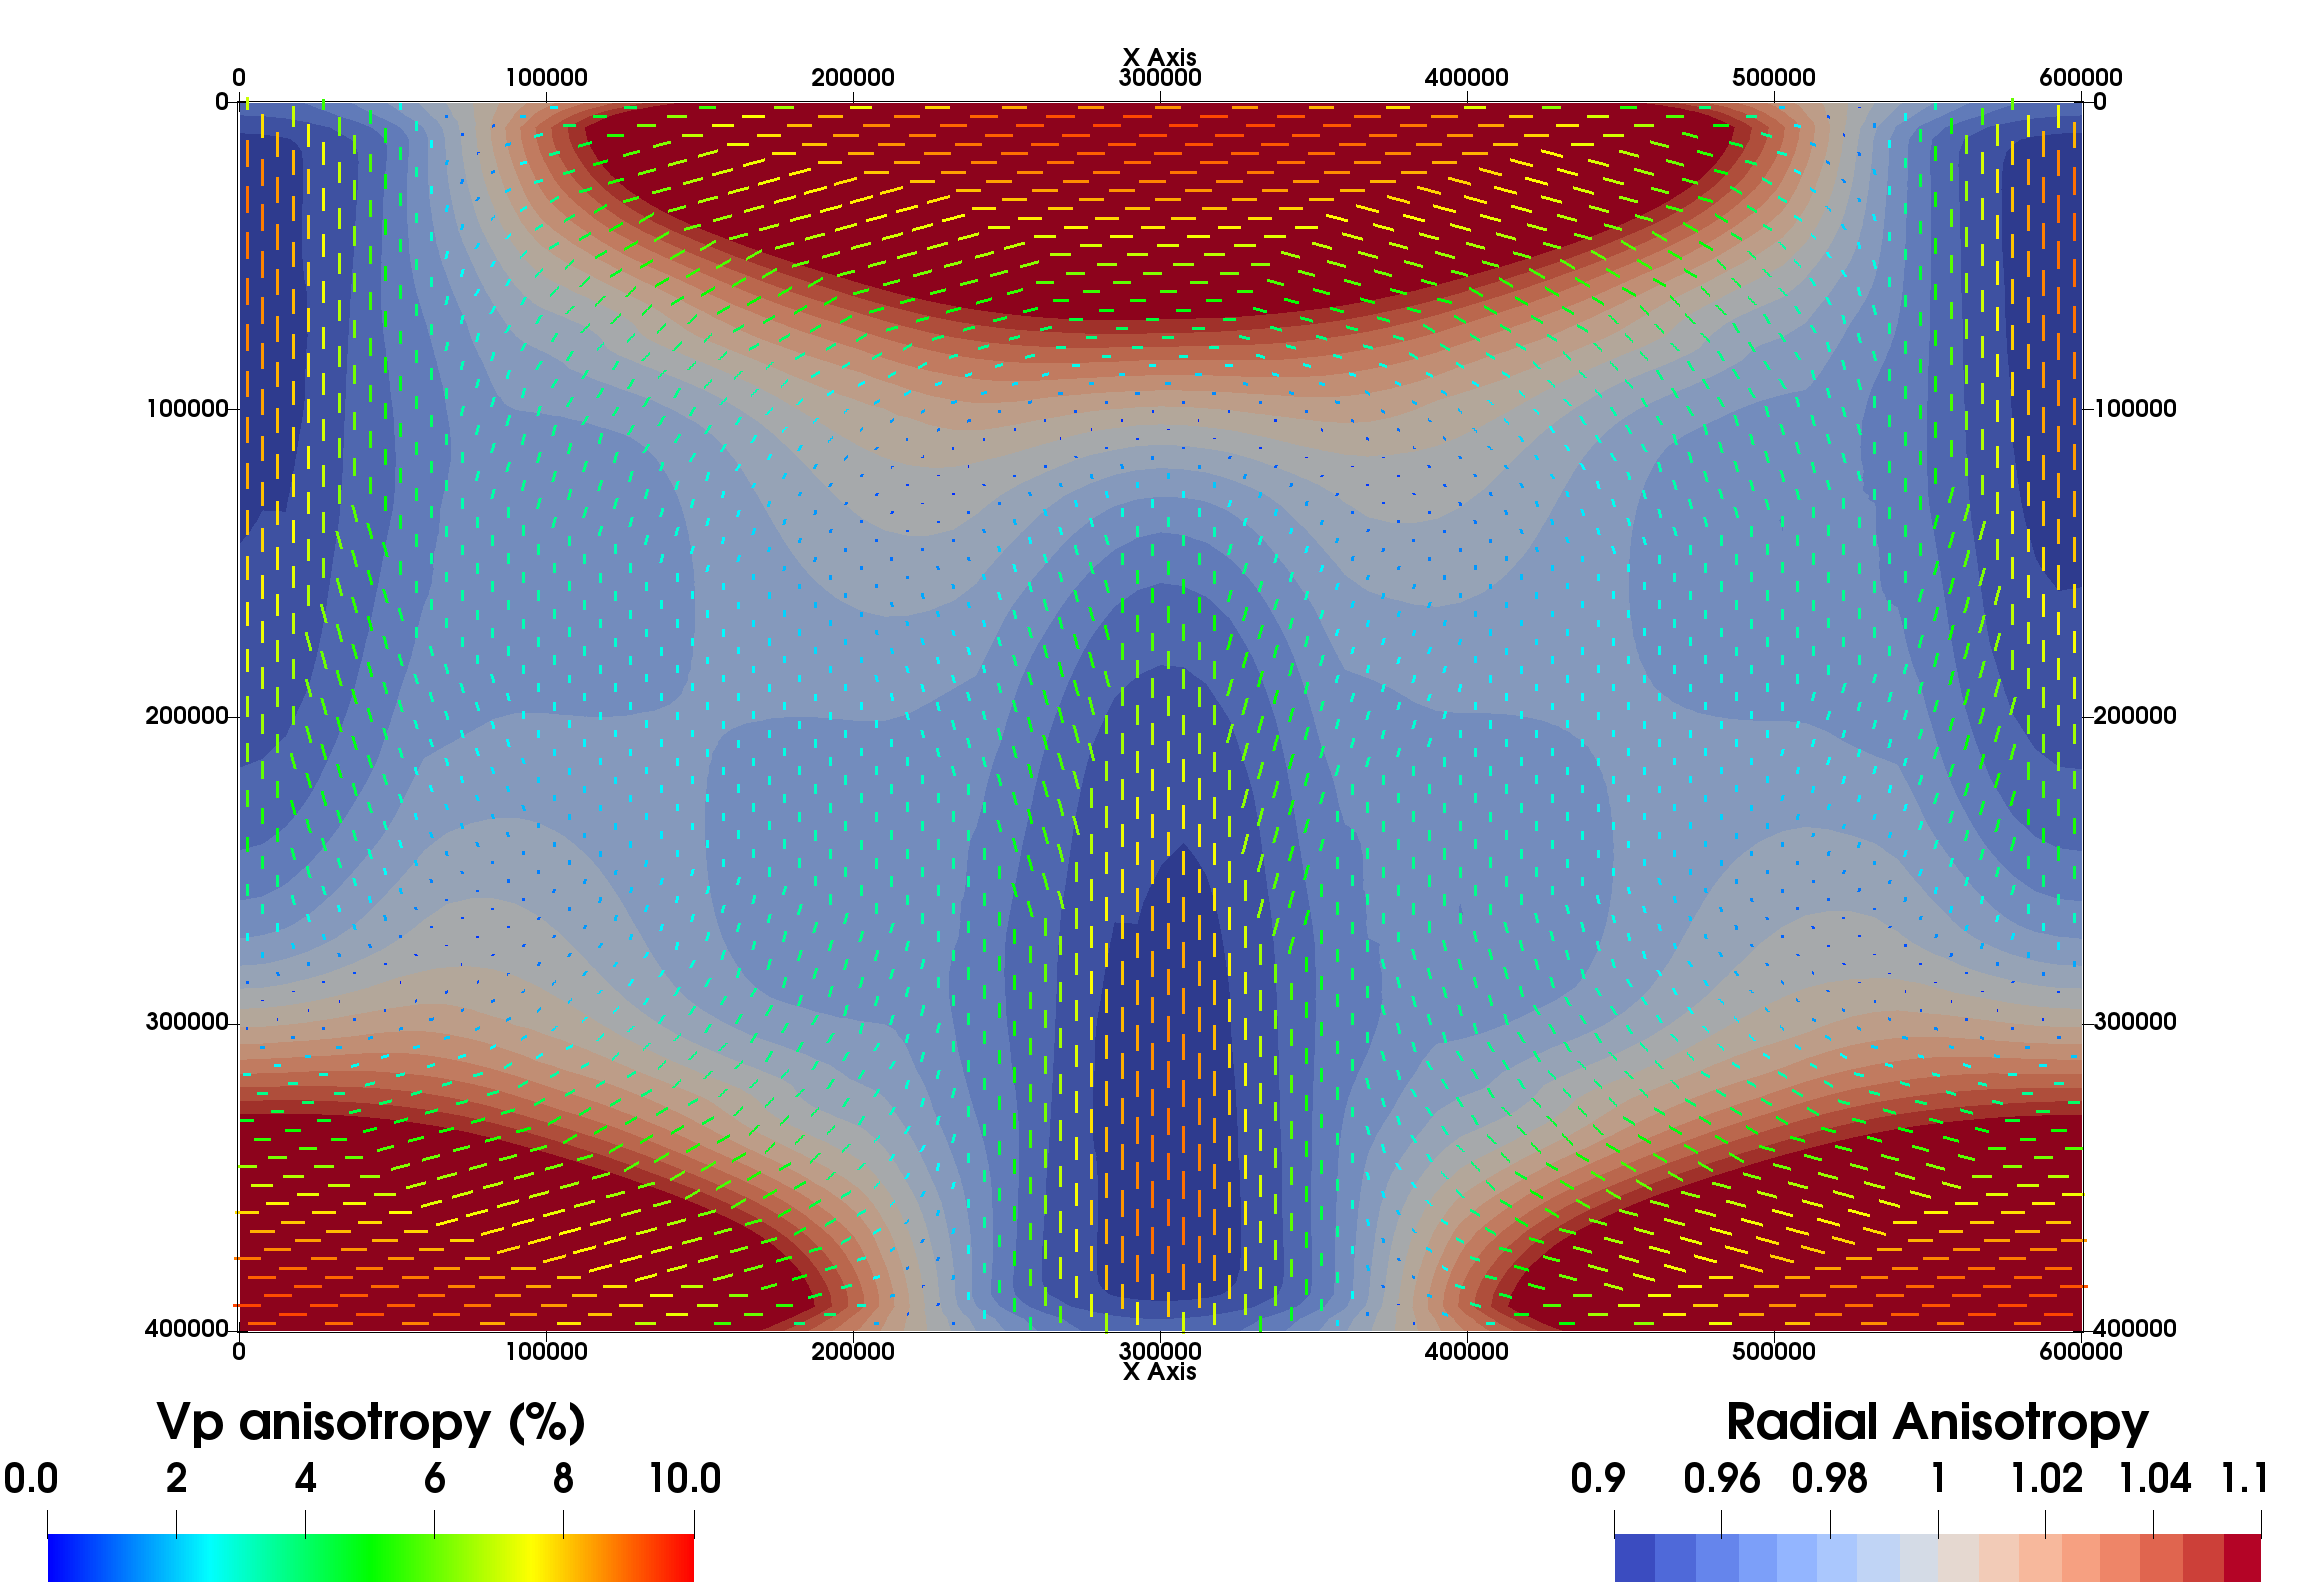
\includegraphics[width=1.0\textwidth]{cookbooks/2Dcartesian_convection_white.png}
    \caption{Steady-state convection pattern in cartesian coordinates created with \texttt{cartesiancells.m}. Radial anisotropy with superimposed Vp\textsubscript{max}.\\
    }
    \label{fig:cartesiancells}
\end{figure}

\vfill % Fill the rest of the page with whitespace

\section{Steady-state subduction in 2D polar coordinates}
\label{section:cookbook_2Dsubduction}

\texttt{DIRECTORY: /2Dpolar\_subduction}
\\
\\
Modeling the elastic properties in oceanic settings is fundamental to constrain the development of seismic anisotropy with formation, ageing and subduction of the oceanic lithosphere.\\  
Oceanic plate formation at the ridge and subsequent subduction at the trench is modelled in 2D polar coordinates with a modified version of the petrological-thermo-mechanical code \textbf{I2VIS} \citep{gerya2003pepi}. The domain is $(\phi,r)=(0-40^{\circ},5671-6371 km)$ and discretized with 1001x351 nodes, the ridge-trench distance is $25^{\circ}$, and a constant plate velocity of 4 cm/yr is imposed. 
The bottom boundary is open, and free slip is imposed on the other 3 boundaries. Free-surface is simulated with a 30 km thick air-layer.\\
The initial temperature field is defined by a constant temperature in the air layer (273 K), the half-space cooling model in the upper (20 Myr) and lower (0-62.5 Myr) plates, and a $0.5 K/km$ adiabat with a mantle potential temperature of $1540 K$.\\ 
The rheology is visco-plastic, and a composite low-T/diffusion/dislocation creep mechanism accommodates viscous deformation. Partial dry melting is simulated beneath the ridge according to parametrized solidus/liquidus curves (Fig. \ref{fig:meltviscosity}).\\ 

\begin{figure}
    \centering
    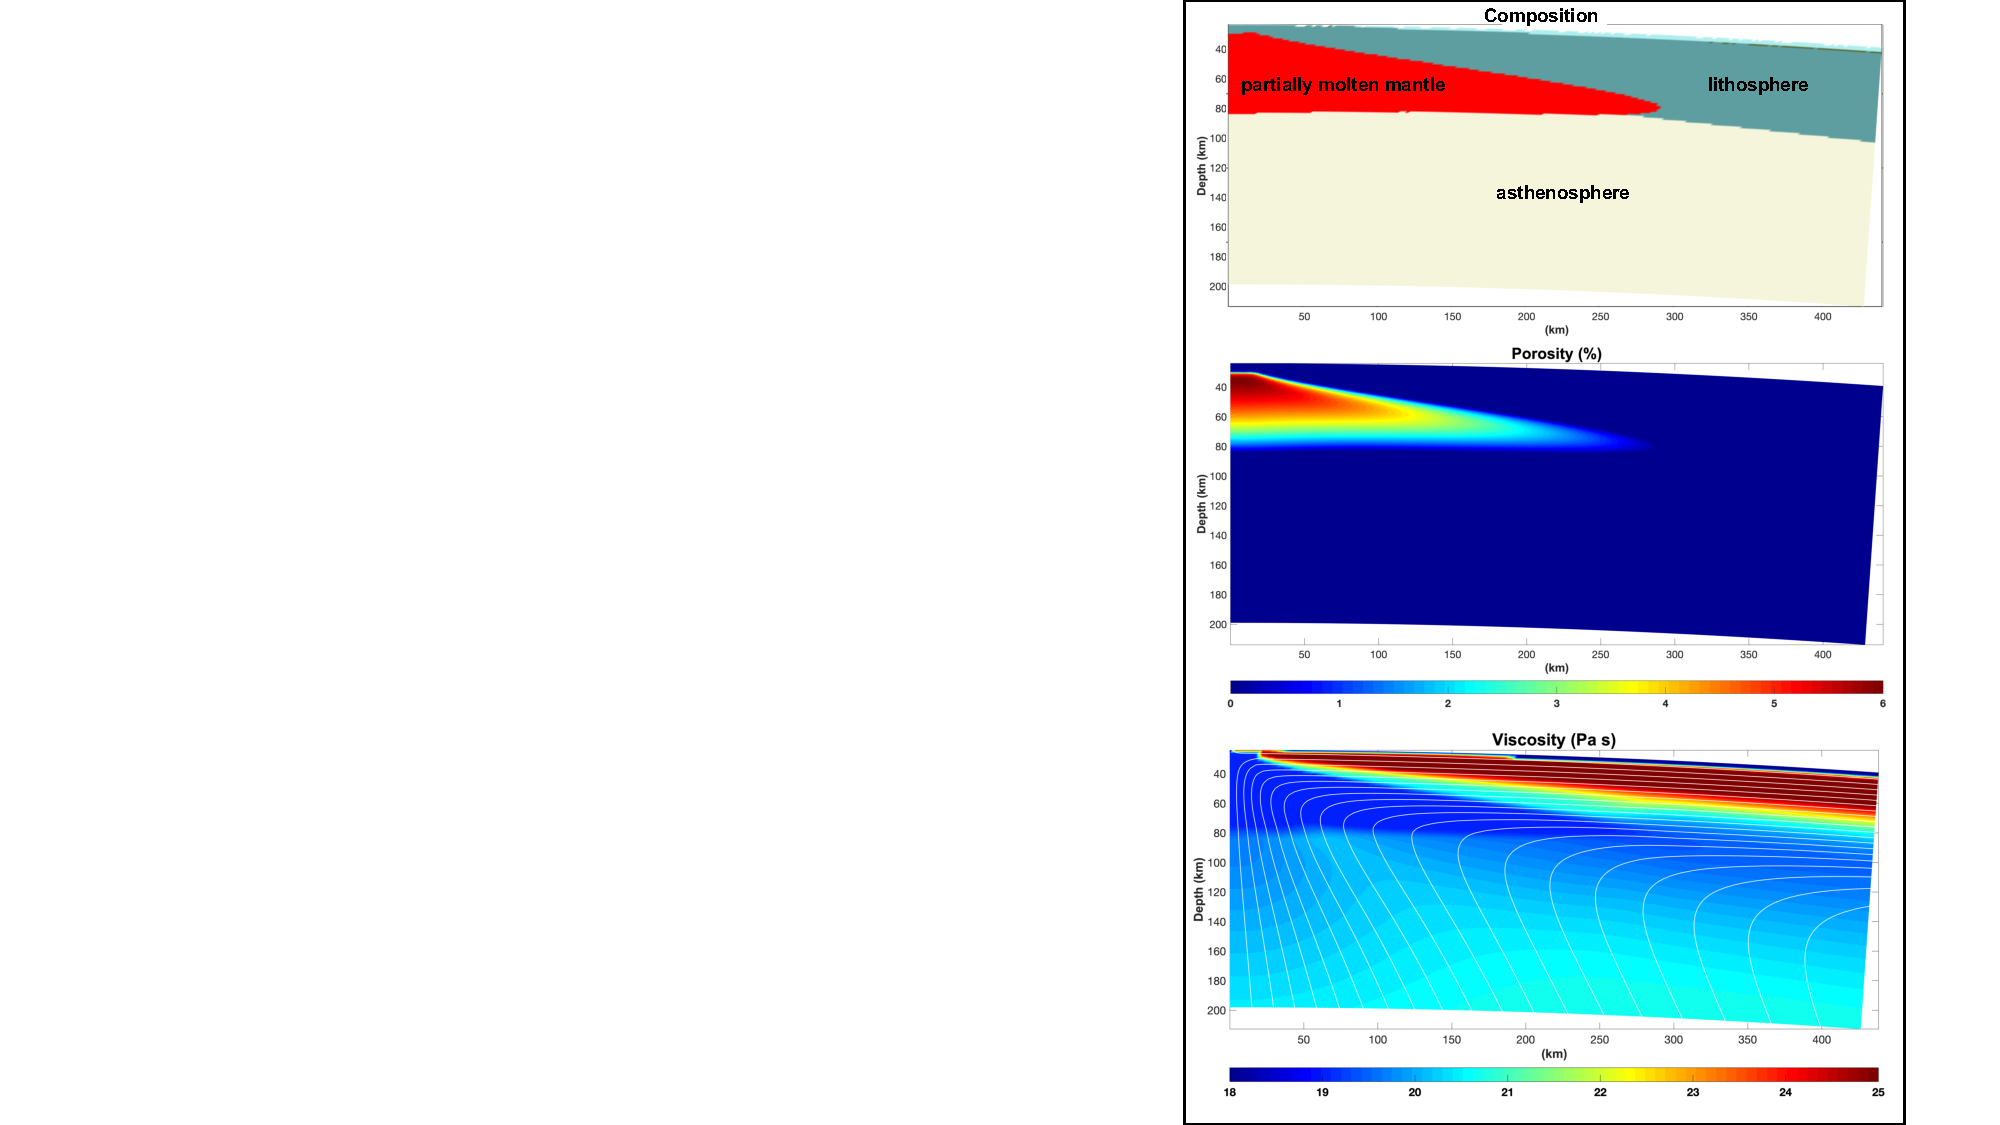
\includegraphics[width=0.9\textwidth]{EXEV/Melt+Viscosity.pdf}
    \caption{Close up of composition, melt fraction and viscosity (with superimposed the streamlines, white lines) of a 2D model of ridge dynamics and oceanic plate formation in polar coordinates.  
    }
    \label{fig:meltviscosity}
\end{figure}

The mantle fabrics are computed assuming steady-state conditions for 100 Myr, which is the time required by the crystal aggregates to move from the trench to the subduction zone, including the initial upwelling and final downwelling episodes.
The isoptropic P-wave distribution for an initial crystal aggregate spacing of 5 km is shown in Fig. \ref{fig:reflectreplicate} .\\

In order to check the role of melt-bearing cracks in seismic anisotropy, the mantle porosity has been saved in \texttt{dsd080melt.h5} and the SPO modelling has been activated in \texttt{viztomo\_input\_spo.dat} as shown in Fig. \ref{fig:extrinsic_anisotropy} for different SPO parameters defined in \texttt{\viztomotitle{}/spo\_input.dat}. 
By setting \fonts{spomod = 3} in \texttt{viztomo\_input.dat} and copying files \texttt{dsd080melt.h5} and \texttt{vtp0080.h5} in the output directory where the file \texttt{Cijkl0080.h5} is located, it is then possible to superimpose the effect of melt-bearing cracks on that due to LPO.


\begin{figure}
    \centering
    \includegraphics[width=0.9\textwidth]{EXEV/Anisotropy.pdf}
    \caption{Radial anisotropy with superimposed the orientation of Vp\textsubscript{max} (left) and TI axis (right) for the model in Fig. \ref{fig:meltviscosity}. In the top row the anisotropy is due to exclusively the strain-indcued LPO (AG-type olivine fabric) estimated with \drexmtitle{}, while in the underneath rows the LPO fabrics are superimposed with SPO fabrics due to the presence of melt. SPO control parameter used are \fonts{spomod = 3}; \fonts{meltspomod = 1}. The inclusions aspect ratio is indicated on the leftmost colums; \fonts{$\phi\textsubscript{SPO}$} is zero everywhere except in the second last row (-30$^{\circ}$). Note that for the penny-shaped inclusions (bottom row) the Vp\textsubscript{max} orientation is randomly oriented in the inclusion flat plane. The TI axis is normal to the flat inclusions, and parallel when cylindrical (second row).
    }
    \label{fig:extrinsic_anisotropy}
\end{figure}

\vfill % Fill the rest of the page with whitespace

\section{Steady-state global scale convection in 2D polar coordinates}
\label{section:cookbook_2Dconvection}

\texttt{DIRECTORY: /2Dpolar\_convection}

A 2D incompressible flow field in cylindrical coordinates is given by the following analytical solution, whereby the radial and tangential velocities are: \\
\begin{center}
    $V_r(\phi,r) = V_{r0}\cos(k_\phi\phi/2)\sin(k_r\pi r')$ \\
    $V_\phi(\phi,r) = -V_{\phi0}(r)\sin(k_\phi\phi/2)\cos(k_r\pi r')$ \\
    $V_{\phi0}(r) = 2V_{r0}/k_\phi[\tan(k_r\pi r') +  k_r\pi r/\Delta R )]$, \\
    $r' = (r - R_{min})/\Delta R$, \\
\end{center}

where $\phi$ and $r$ are longitude and radial distance, $V_{r0}$ a constant, $k_\phi$ and $k_r$ are the tangential and radial wave numbers, $\Delta R = R_{max} - R_{min}$, with $R_{min}$ and $R_{max}$ the bottom and top radial coordinate. 

Pressure distribution is:
\begin{center}
    $P(r) = P_0 + (R_{max} -r)/\Delta R \cdot P_1$ 
\end{center}
Temperature distribution is:
\begin{center}
    $T(\phi,r) = T_c(r) + dT (\phi,r)$

    $T_c(r) = T_0 + (R_{max} -r)/\Delta R \cdot T_1$

    $dT(\phi,r) = dT_{max}*V_r(\phi,r)/V_{r0}$
\end{center}
where $P_0$, $P_1$, $T_0$, $T_1$, $dT_{max}$, $V_{r0}$ are constants.

The \fonts{V}, \fonts{P} and \fonts{T} fields are computed with the \matlabtitle{} script \texttt{polarcells.m} and saved to \texttt{vtp0001.h5} as a function of the numerical resolution, radial and tangential wave numbers, and P-T conditions. 
The mantle fabrics computed with \drexmtitle{} in steady-state conditions for 100 Myr and visualized with \viztomotitle{} are shown in Fig. \ref{fig:polarcells} 
In global convection models, the vertical boundary should be open, i.e., the domain should be periodic along the tangential direction, thus:\\

    \begin{itemize}
        \item[] \fonts{dimensions = 2} 
        \item[] \fonts{cartspher = 2} 
        \item[] \fonts{x1periodic = 1} 
    \end{itemize}


\begin{figure}
    \centering
    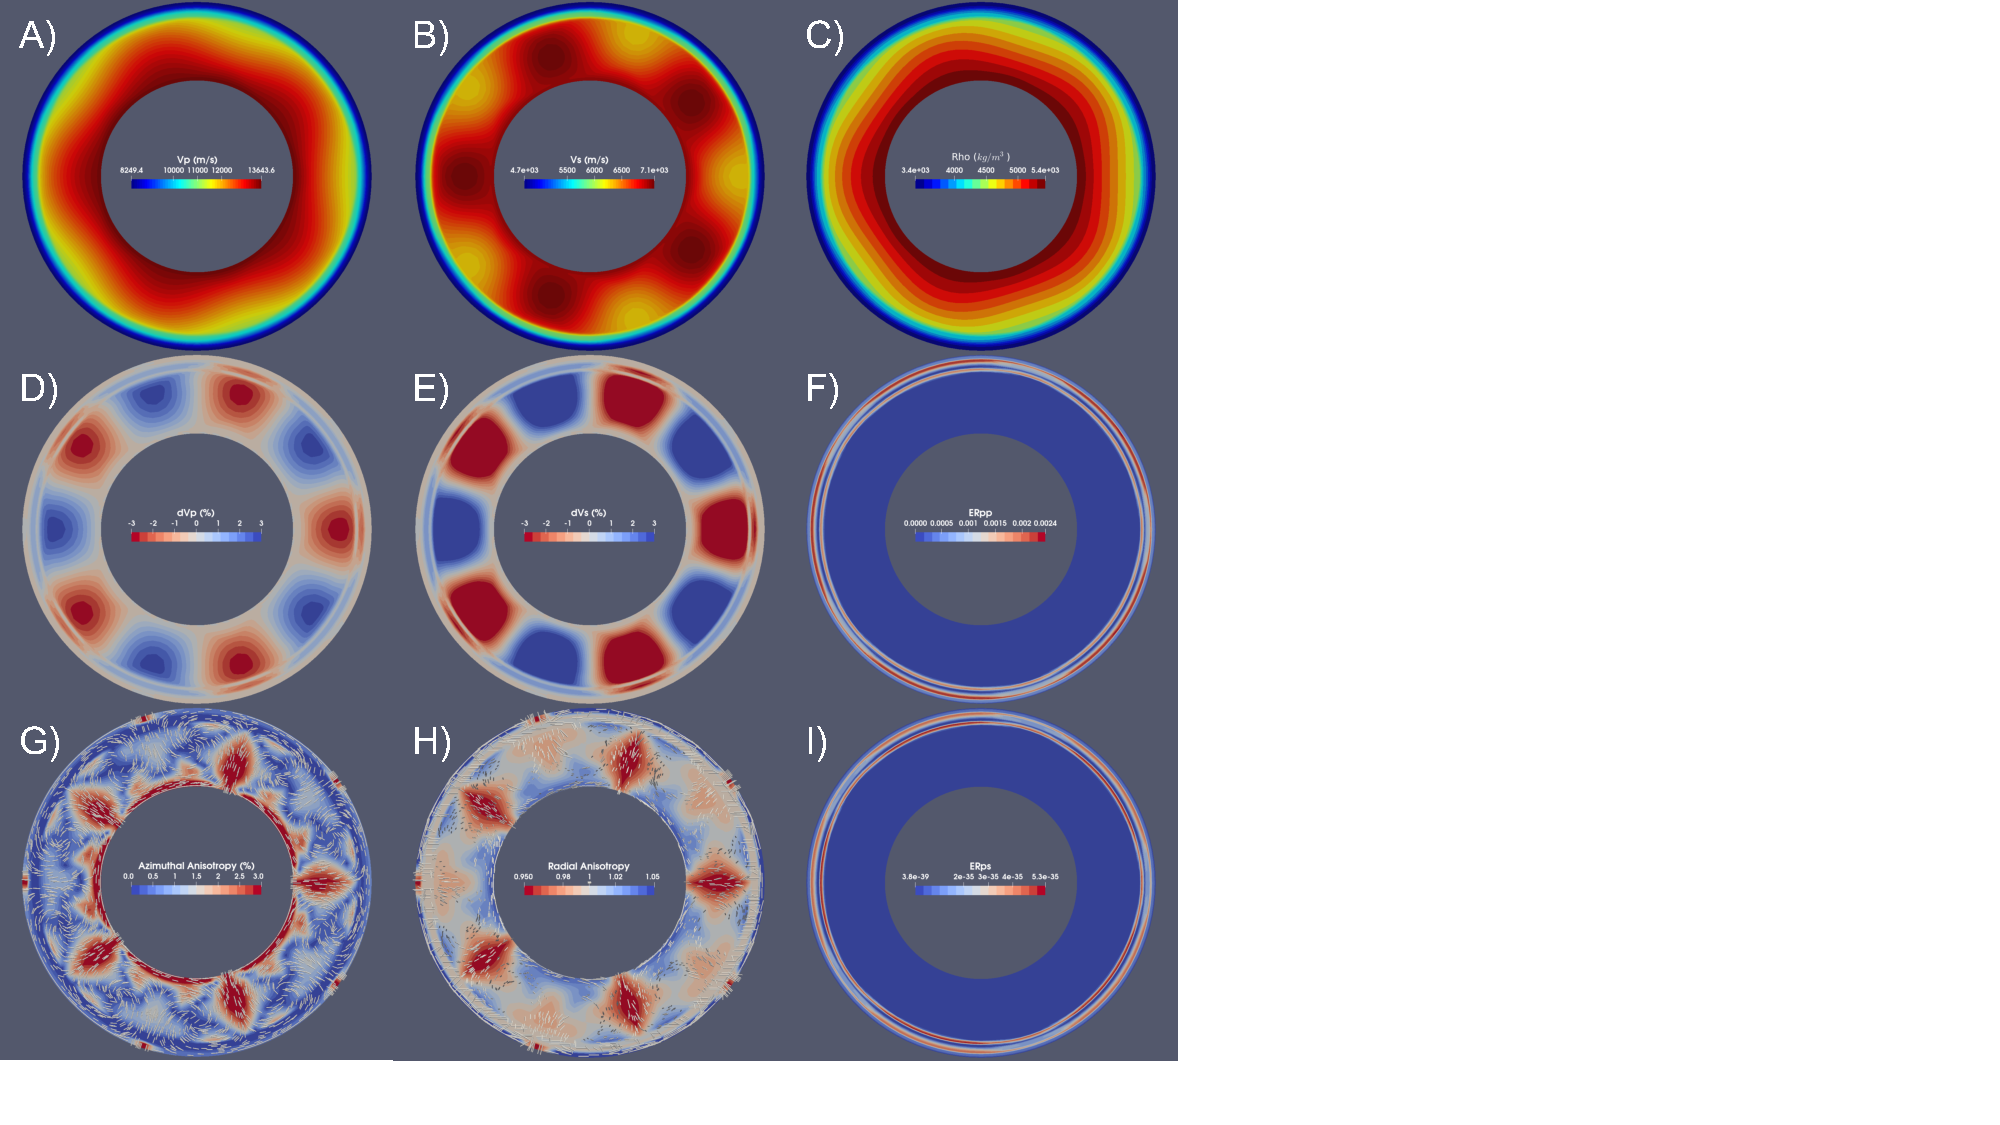
\includegraphics[width=1.0\textwidth]{cookbooks/polarcells.pdf}
    \caption{Steady-state convection patterns in polar coordinates created with \texttt{polarcells.m}. A) P-wave velocity; B) S-wave velocity; C) Density; F) and I) Normalized P-P and P-S reflected energy; D) and E) P- and S-wave anomalies with respect horizonthally averaged velocities. G) Azimuthal anisotropy with superimposed fse\textsubscript{max}; H) Radial anisotropy with superimposed Vp\textsubscript{max}.\\
    }
    \label{fig:polarcells}
\end{figure}

\vfill % Fill the rest of the page with whitespace

\section{Sinking slab in 3D cartesian coordinates}
\label{section:cookbook_3Dcartesian_sinking}

\texttt{DIRECTORY: /3Dcartesian\_sinkingslab}

The flow field of a sinking cold horizontal slab is computed with the petrological-thermo-mechanical code \textbf{I3MG} \citep{gerya2003pepi}.
The domain is $(x,y,z)=(2000,1000,2000) km$ and discretized with 37x37x37 nodes, and free slip is imposed on all boundaries. The initial temperature field is defined by the half-space cooling model in the 90 km thick, 80 Myr old plate, a constant temperature of 473 K in the 100 km thick, 800 km long and 400 km wide slab centered with respect to the horizontal plane and initially at depth of 200-300 km, and a $0.5 K/km$ adiabat in the surrounding mantle with a potential temperature of $1540 K$. \\
The rheology is visco-plastic, and a composite low-T/diffusion/dislocation creep mechanism accounts for viscous deformation. An increase in viscosity is set at the 660 km depth discontinuity. \\

The mantle fabrics are computed using 20 \vtptitle files, for a total of 2 Myr. An initial (fossil) fabric is imposed on the horizontal slab with fast directions lying in the horizontal plane at $45^{\circ}$ from the x and z axes (Fig. \ref{fig:sinkinkslab_cartesian}.

\begin{figure}[ht]
    \centering
    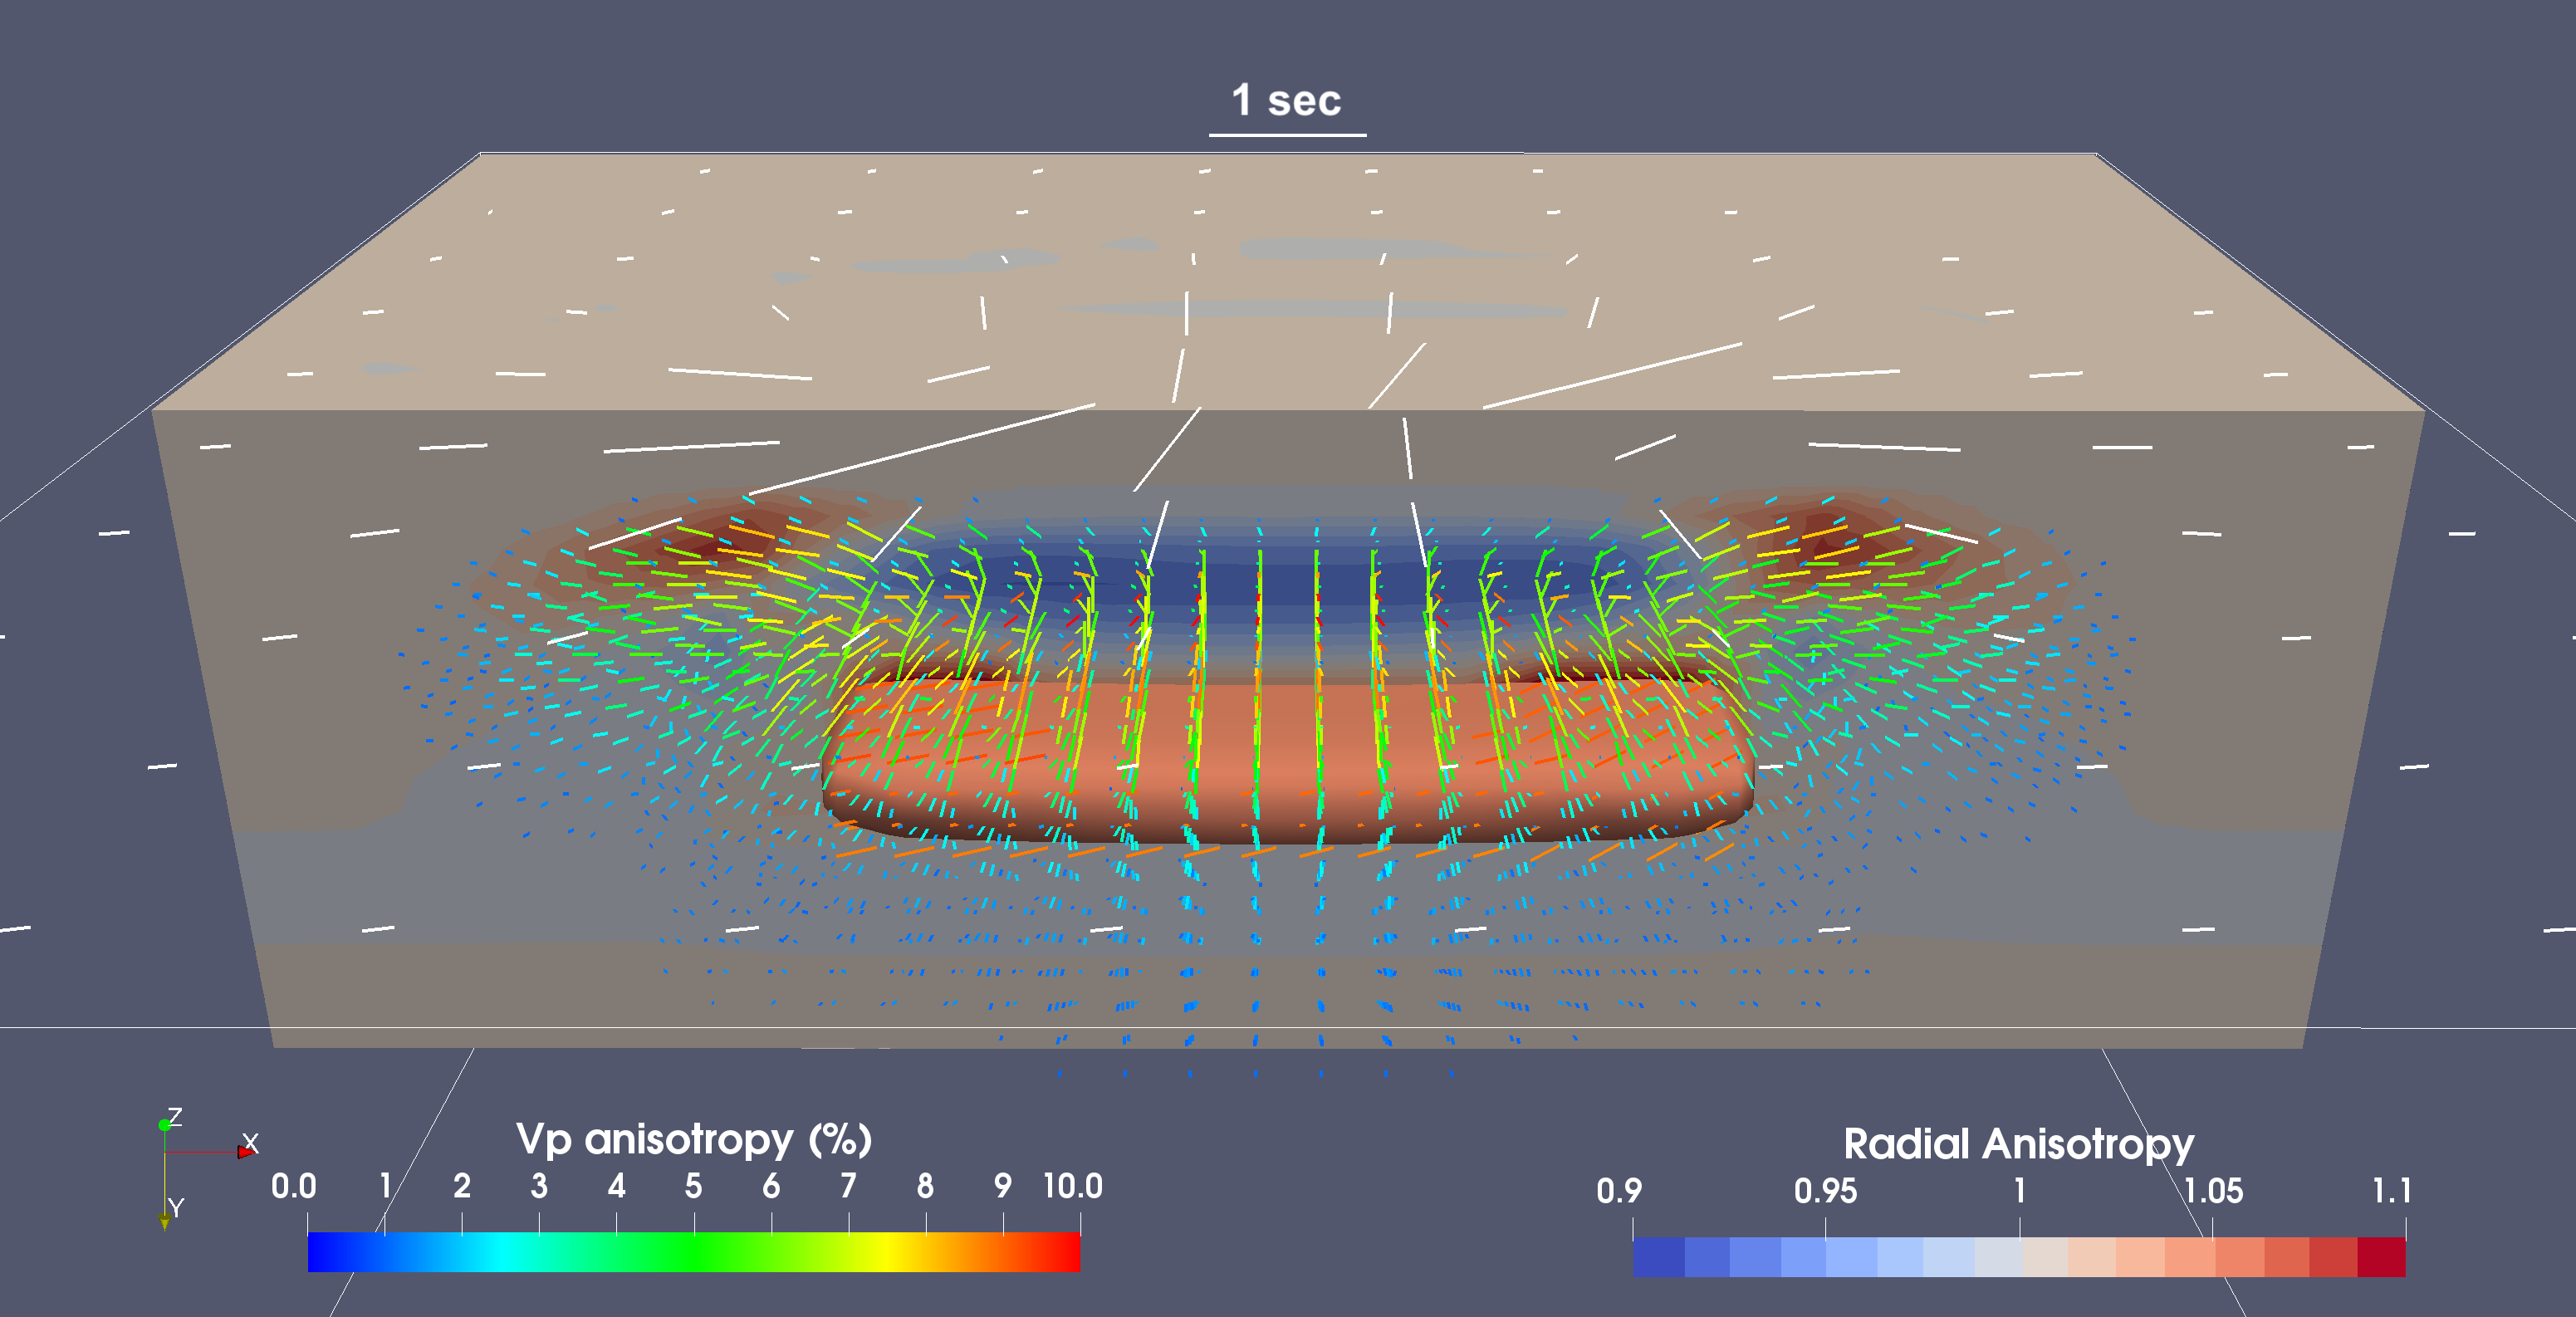
\includegraphics[width=1.0\textwidth]{cookbooks/3Dcartesian_sinkingslab2.png}
    \caption{Time-dependent flow model of a sinking horizontal slab (contoured by the pink surface) in 3D cartesian coordinates. Radial anisotropy is shown on upper half of the image, while Vp\textsubscript{max} in the lower half. The white bars at the surface show SKS splitting, with length proportional to the delay time. The fossil fabric is shown by the orange bars close to the slab. Areas of sub-horizontal flow are characterized by positive radial anisotropy and sub-horizontal Vp\textsubscript{max}.\\
    }
    \label{fig:sinkinkslab_cartesian}
\end{figure}

\vfill % Fill the rest of the page with whitespace

\section{Sinking slab in 3D spherical coordinates}
\label{section:cookbook_3Dspherical_sinking}

\texttt{DIRECTORY: /3Dspherical\_sinkingslab}

An analogous model setup for the sinking slab in cartesian coordinates has been run in spherical coordinates using a modified version of \textbf{I3MG}. Differently form the previous example, the horizontal coordinates in the input files are now given in degrees rather in meters. The domain is $(\phi,r,\theta)=(80-100^{\circ},5371-6371 km,80-100^{\circ})$, and the slab is $8^{\circ}$ long and $4^{\circ}$ wide (Fig. \ref{fig:sinkinkslab_spherical}).
This model is used as an example for the seismic inversions performed with \syntomotitle{} (see \ref{SynTomo:Example}).

\begin{figure}[ht]
    \centering
    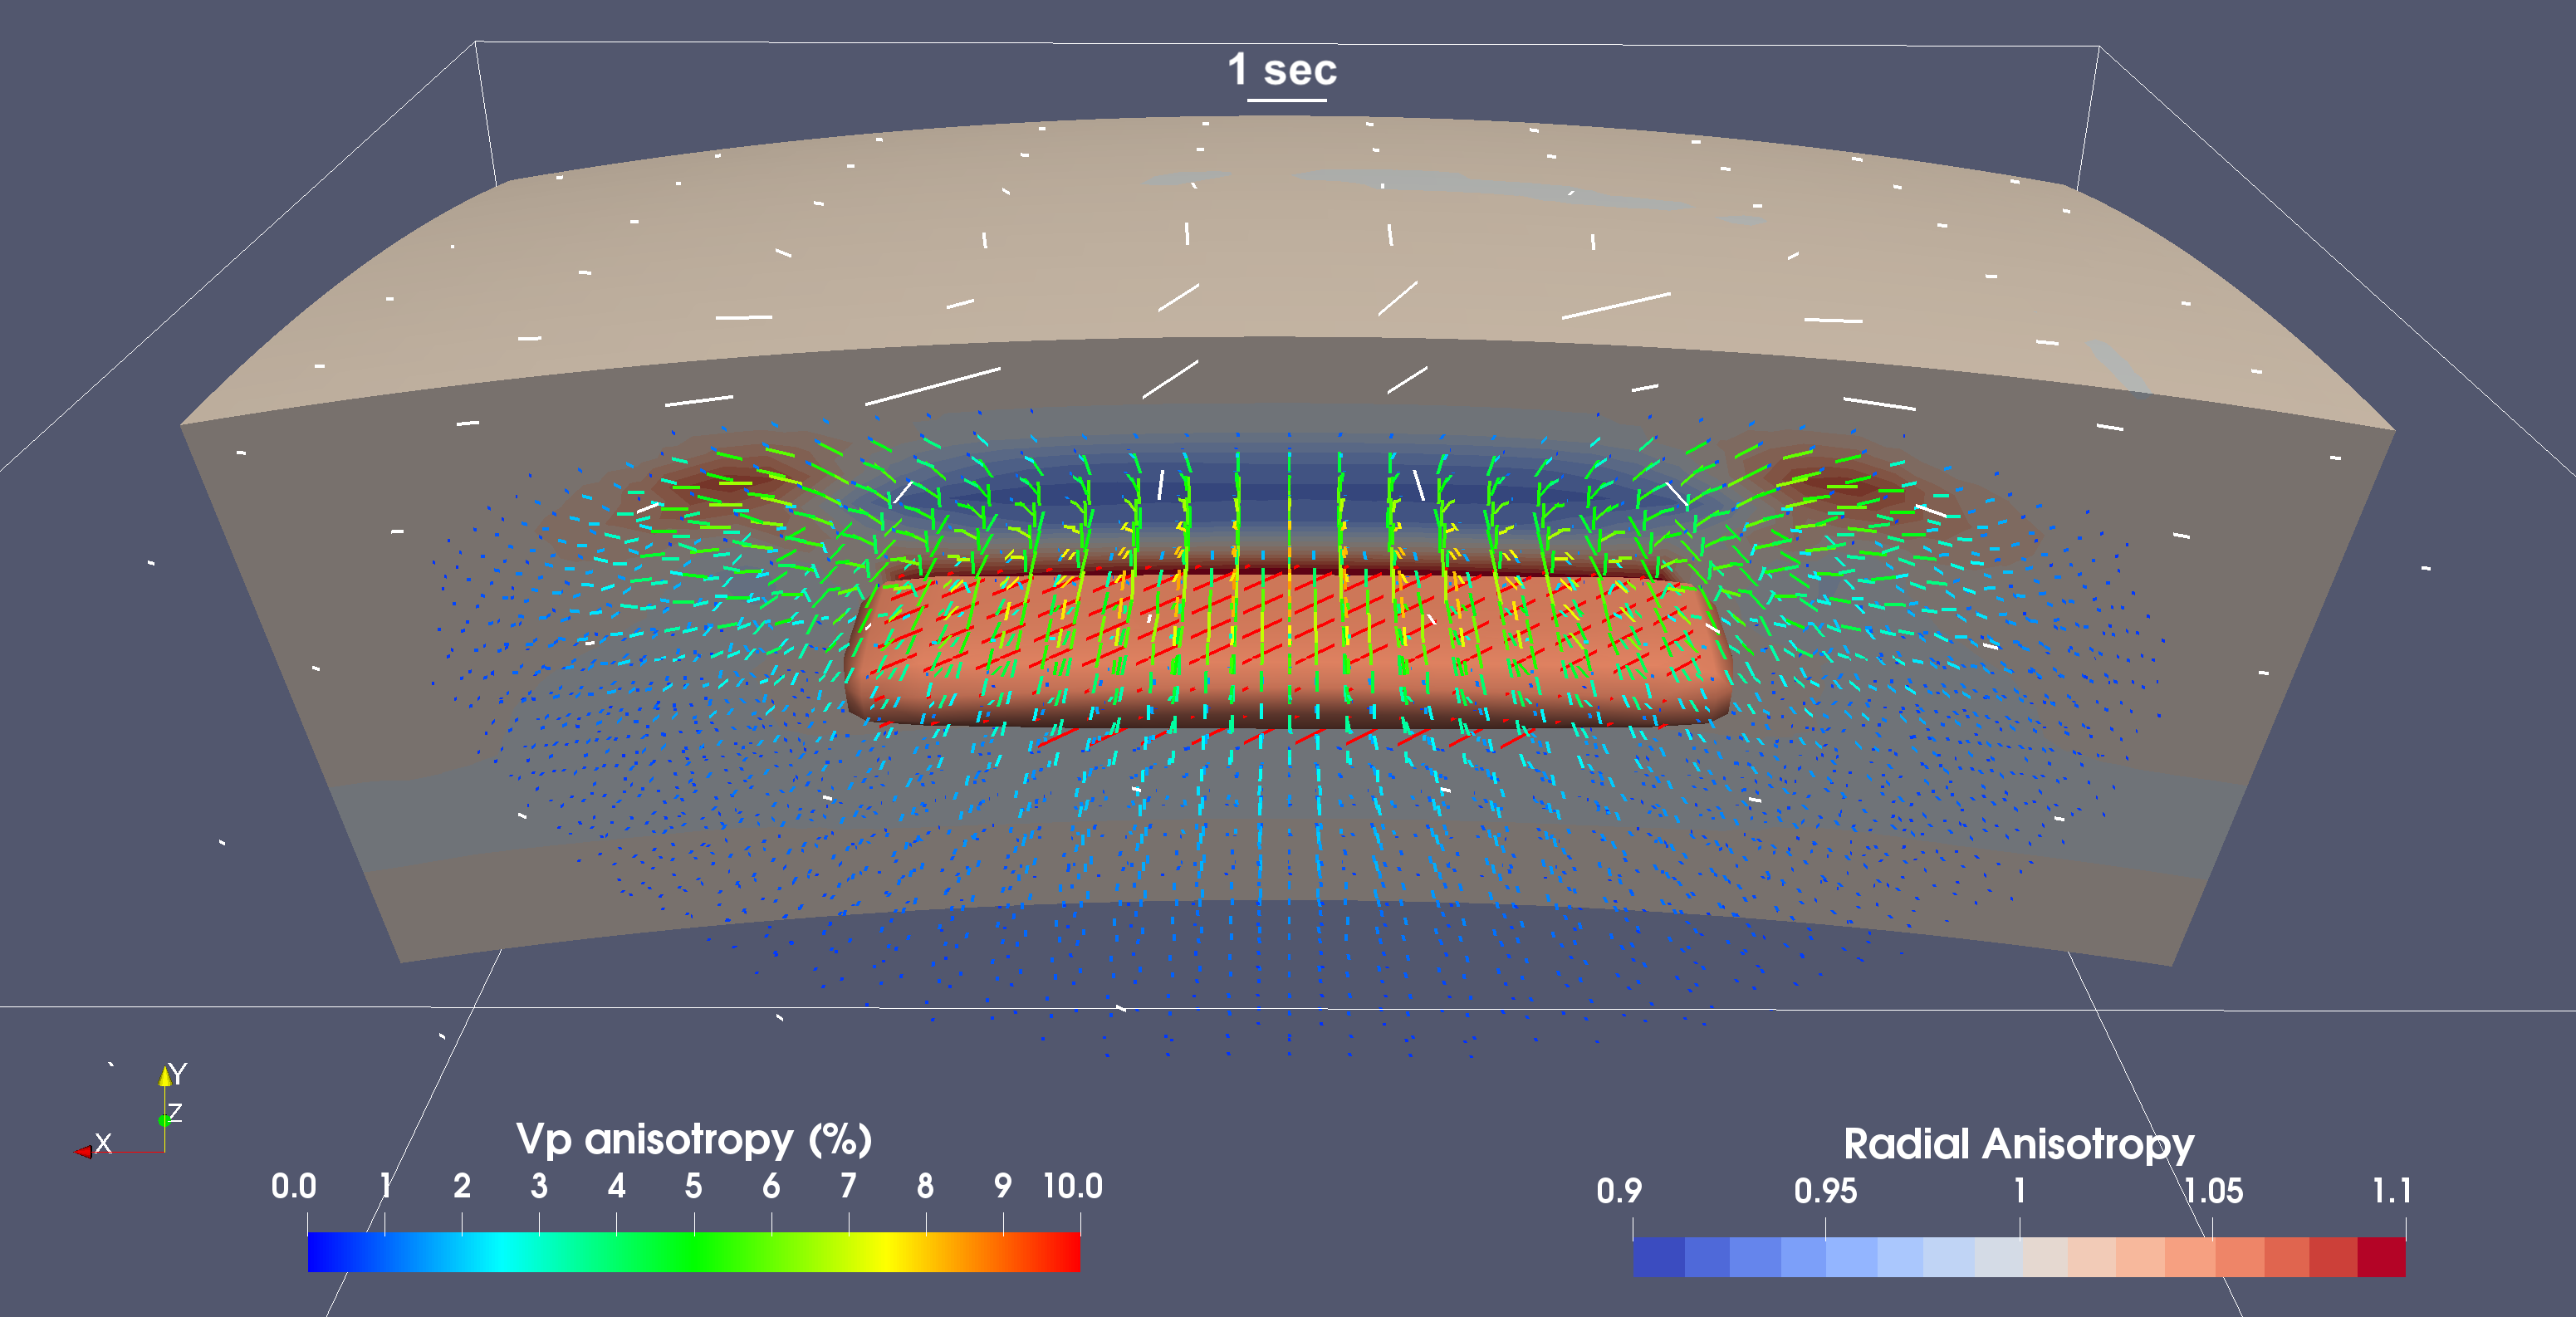
\includegraphics[width=1.0\textwidth]{cookbooks/3Dspherical_sinkingslab3.png}
    \caption{Time-dependent flow model of a sinking horizontal slab (contoured by the pink surface) similar to \ref{fig:sinkinkslab_cartesian} but in spherical coordinates.\\
    }
    \label{fig:sinkinkslab_spherical}
\end{figure}

\vfill % Fill the rest of the page with whitespace

\section{Steady-state global scale convection in 3D spherical coordinates}
\label{section:cookbook_3Dspherical_global}

\texttt{DIRECTORY: /3Dspherical\_global}

The global scale flow field has been simulated with a modified version of \textbf{I3MG} that solves the fundamental conservation equations of continuum mechanics in spherical coordinates using the Yin-Yang grid, an overset grid composed of to identical component grids that are combined in a complementary way to cover a spherical surface with partial overlap on their boundaries \citep{kageyama2004g3}. Each component grid is a low-latitude part of the latitude-longitude grid, and therefore the grid spacing is quasi-uniform. \\
The model is non-dimensional and discretized with 149x101x53x2 nodes, the initial temperature field is characterized by a conductive thermal gradient plus a thermal perturbation that varies along the radial direction with a sinusoidal pattern and laterally with cubic symmetry. The Rayleigh number is 14000, which yields a steady-state flow pattern.\\
In spherical coordinates, the mantle fabrics and their advection is computed by means of the Yin-Yang grid.  
The grids span over $-3\pi/4 -d\phi \leq \phi \leq 3\pi/4 + d\phi$ and $\pi/4 -d\theta \leq \theta \leq 3\pi/4  + d\theta$, where $d\phi$ and $d\theta$ are small buffers that ensure grids overlap, and usually taken equal to the grid spacing.\\
The longitudinal, radial and colatitudinal velocity components (in m/s or its adimensional counterpart), as well P,T and Fd, of the geodynamic model should then be interpolated to the nodes of the two grids as shown in the \matlabtitle{} script: \\
\texttt{/\drexmtitle/make\_HDF5\_vtp\_files/makevtpfiles\_yinyang.m}.\\
In global convection models, the vertical boundaries should be open, thus \fonts{x1periodic} and \fonts{x3periodic} must be set to $1$. As such, the Yin-Yang grid is activated in the \drexmtitle{} parameter input file by setting:
    \begin{itemize}
        \item[] \fonts{dimensions = 3} 
        \item[] \fonts{cartspher = 2} 
        \item[] \fonts{x1periodic = 1} 
        \item[] \fonts{x3periodic = 1}
    \end{itemize}

The \drexmtitle{} parameter input file is configured with adimensional \fonts{timemax} and distances, and such that the fabrics are computed only for upper mantle aggregates and without scaling the single crystal elastic tensors by the local P-T conditions. With an aggregate spacing of 80-90 km, about 1.3 millions of aggregates are distributed throughout the mantle, such that about 115 GB of memory needs to be allocated.
The azimuthal anisotropy related to these fabrics is shown in Fig. \ref{fig:globalconvection}, while the P-wave anomalies are shown in the manual cover image.

\begin{figure}[ht]
    \centering
    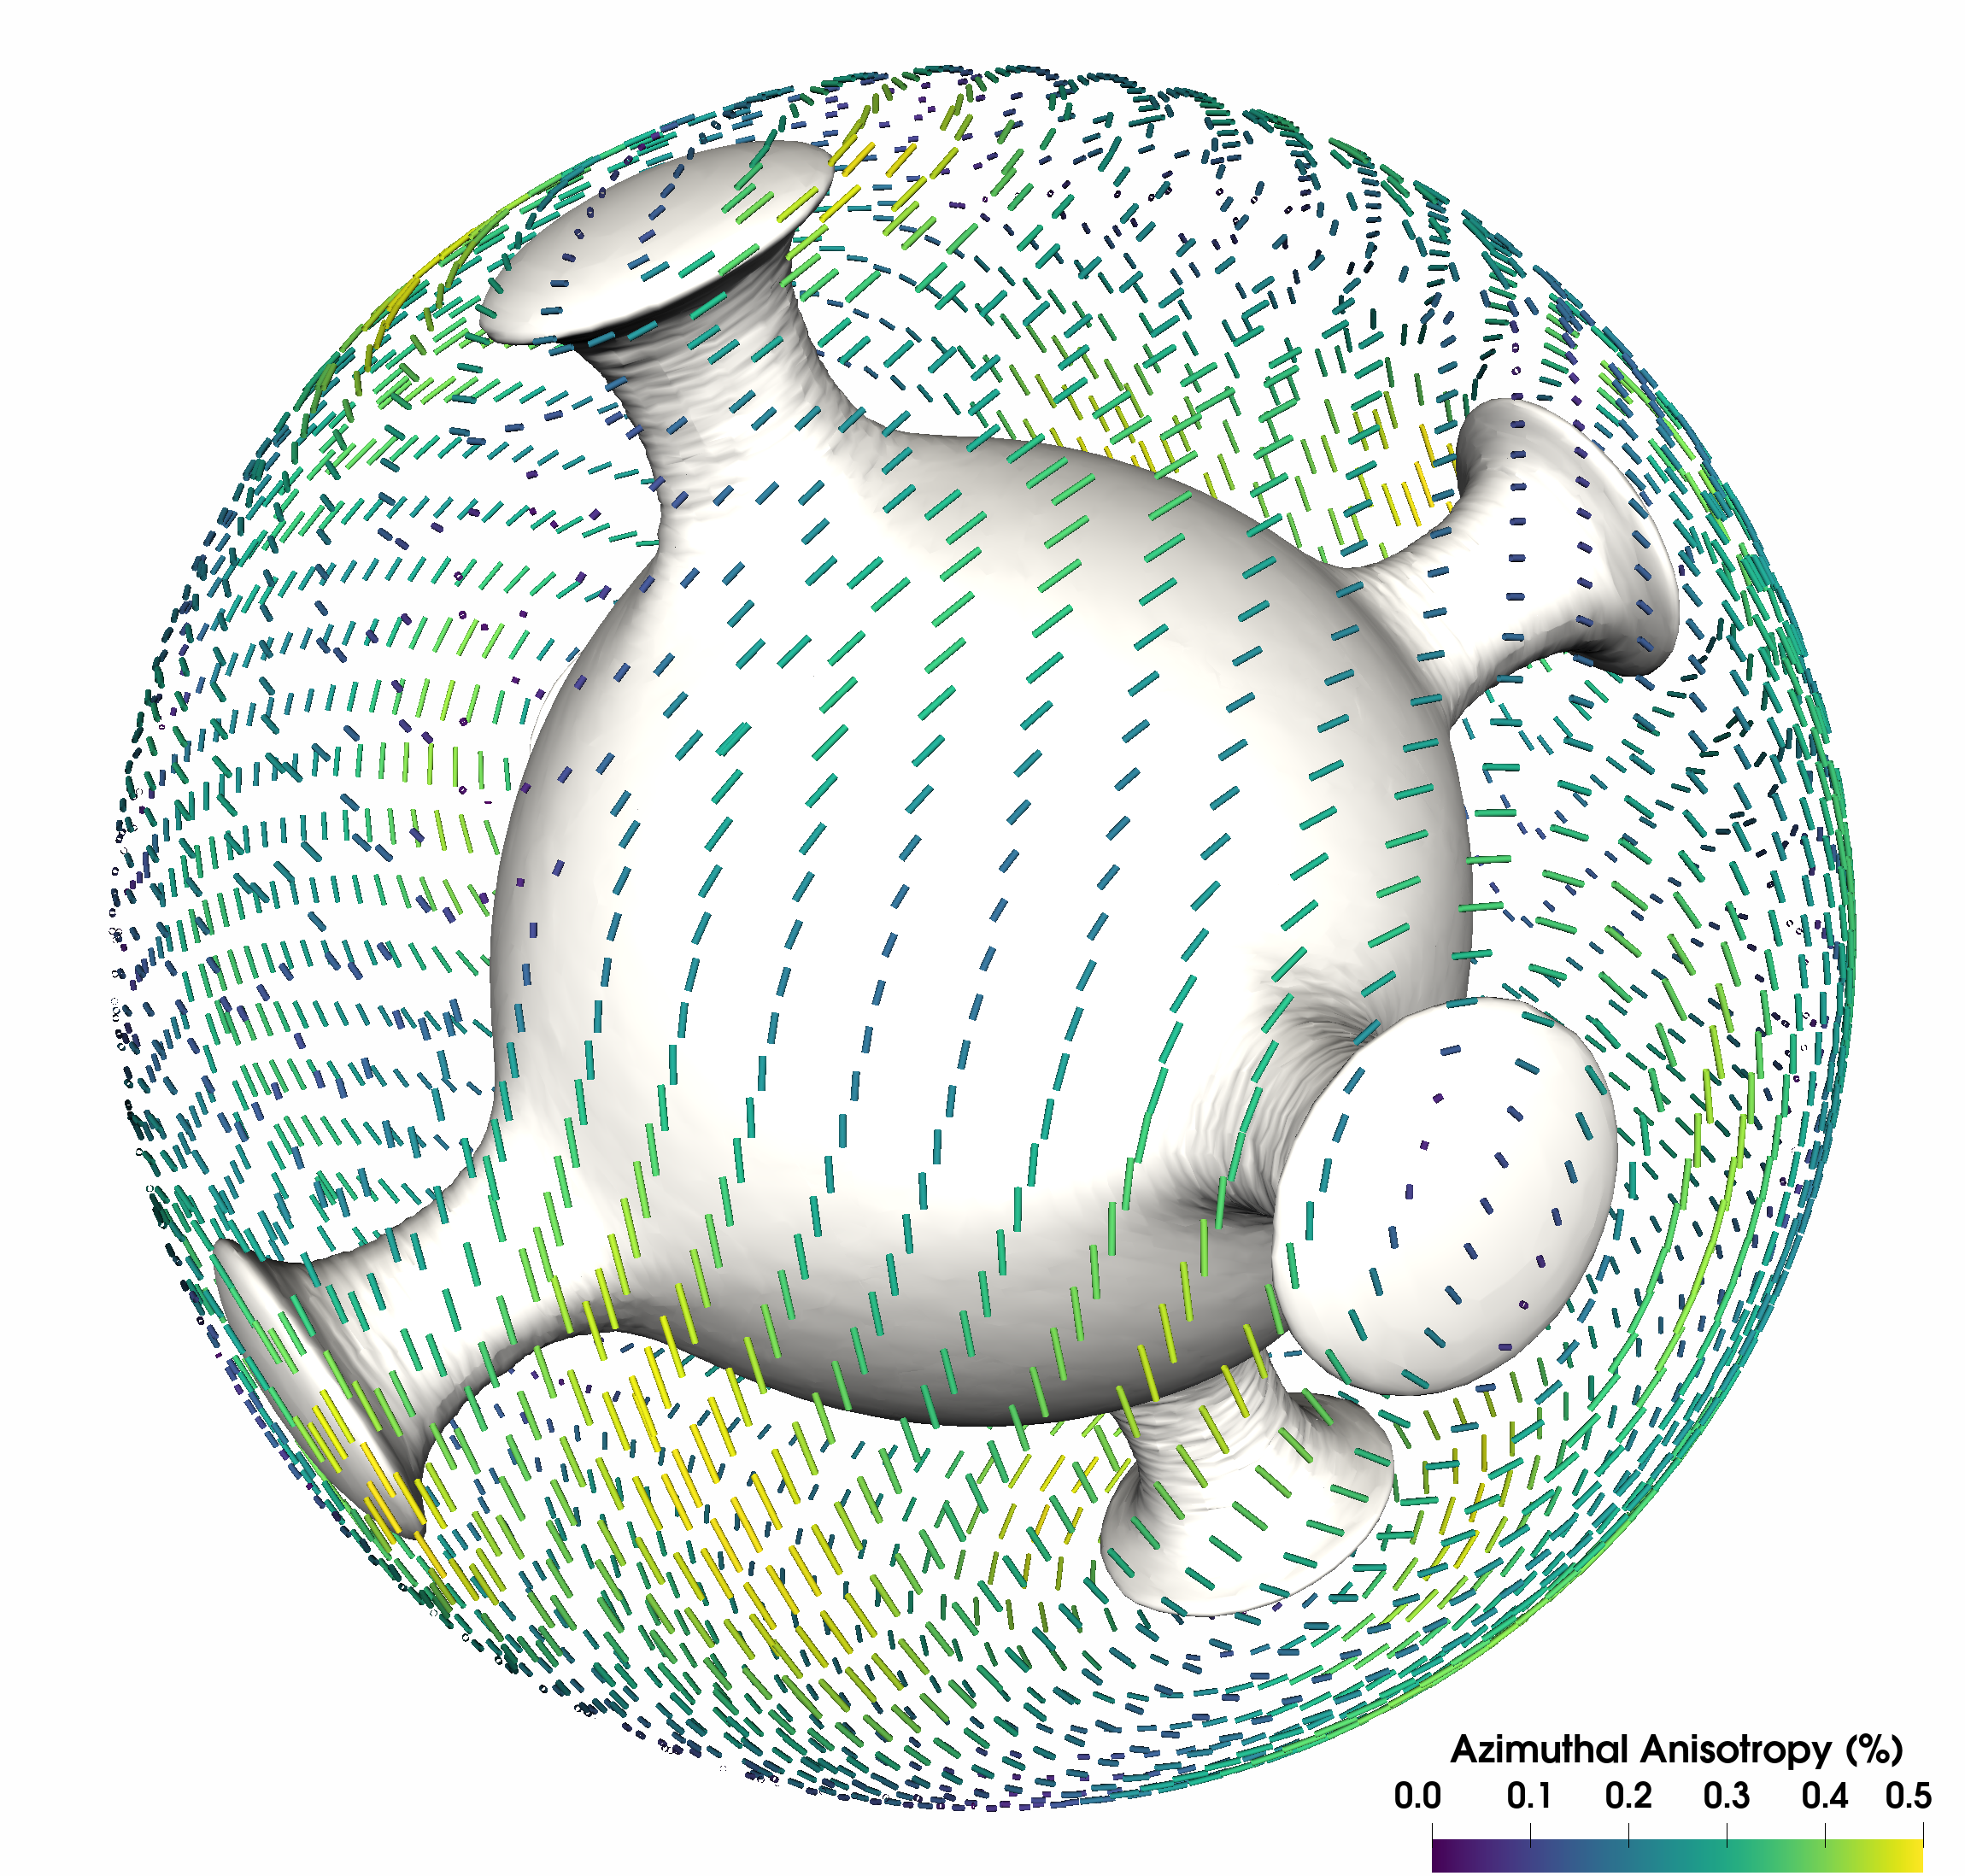
\includegraphics[width=1.0\textwidth]{cookbooks/3Dspherical_cubic2white.png}
    \caption{Steady-state global convection patterns in 3D spherical coordinates. The contours are T = 0.5. The bars indicate azimuthal anisotropy in the upper mantle.\\
    }
    \label{fig:globalconvection}
\end{figure}

\vfill % Fill the rest of the page with whitespace
\bibliographystyle{abbrvnat}
\bibliography{bibs/sample}
\appendix
\renewcommand{\thechapter}{A\arabic{chapter}}
\chapter{Appendix}
\label{chapter:appendix}

\begin{table}[h!]
\caption{Slip systems of abundant anisotropic mantle phases present in \drexstitle{} and \drexmtitle{}}
\centering
\begin{tabular}{|>{\small}p{3.5cm} |c|c|c|c|c|} 
 \hline
 \normalsize{Slip\quad system [uvw](hkl)} & Olivine & Enstatite & Wadleyite & Bridgmanite & post-Perovskite\\ [0.5ex] 
 \hline\hline
 $[100](010)$ & $\star$ & - & $\star$ & $\star$ & $\star$ \\\hline
 $[100](001)$ & $\star$ & - & $\star$ & $\star$ & $\star$ \\\hline
 $[100](011)$ & - & - & $\star$ & - & -\\\hline
 $[100](021)$ & - & - & $\star$ & - & -\\\hline
 $[010](100)$ & - & - & - & $\star$ & $\star$ \\\hline
 $[010](001)$ & - & - & - & $\star$ & $\star$ \\\hline
 $[001](100)$ & $\star$ & $\star$ & - & $\star$ & $\star$ \\\hline
 $[001](010)$ & $\star$ & - & $\star$ & $\star$ & $\star$ \\\hline
 $[001]\{\bar{1}10\}$ & - & - & - & $\star$ & $\star$ \\\hline
 $<\!\bar{1}10\!>\!(001)$ & - & - & - & $\star$ & -\\\hline
 $<\!110\!>\!\{\bar{1}10\}$ & - & - & - & $\star$ & $\star$ \\\hline
 $1/2\!<\!111\!>\!\{101\}$ & - & - & $\star$ & - & -\\\hline
\end{tabular}
\label{table:1}
\end{table}

%\begin{landscape}
\begin{table}[ht]

\caption{\small{Elastic moduli (GPa) and their P–T derivatives of the mineral phases used in this study. Temperature derivatives are scaled by $10^{-2}$ \si{GPa K^{-1}}, while cross derivatives by $10^{-3}$ \si{K^{-1}}}}
\begin{adjustbox}{width=1\textwidth}
\begin{tabu}{p{.13\textwidth} >{\centering}p{0.08\textwidth} p{.20\textwidth} r{.06\textwidth} r{.06\textwidth} r{.06\textwidth} r{.06\textwidth} r{.06\textwidth} r{.06\textwidth} r{.06\textwidth} r{.06\textwidth} r{.06\textwidth} p{0.05\textwidth}}
\toprule
\\
\rowfont{\large}
Mineral & Idx$^\star$ & Moduli & C11 & C22 & C33 & C12 & C13 & C23 & C44 & C55 & C66 & Source$^\dagger$\\[6ex]
\toprule
Olivine & 1 & $M$ & 320.71 & 197.25 & 234.32 & 69.84 & 71.22 & 74.80 & 63.77 & 77.67 & 78.36 & (1)\\
  & & $\partial{M}/\partial{P}$ & 5.41 & 5.26 & 3.78 & 1.88 & 1.53 & 1.60 & 1.08 & 1.42 & 1.80 & (2)\\
  & & $\partial{M}/\partial{T}$ & -4.02 & -3.10 & -3.53 & -1.14 & -0.96 & -0.72 & -1.26 & -1.30 & -1.56 & (1)\\

\midrule

Enstatite & 2 & $M$ & 236.90 & 180.50 & 230.40 & 79.60 & 63.20 & 56.80 & 84.30 & 79.40 & 80.10 & (3)\\
    & & $\partial{M}/\partial{P}$ & 10.27 & 8.87 & 11.7 & 6.22 & 6.63 & 7.26 & 1.23 & 0.75 & 2.78 & (3)\\
    & & $\partial^2{M}/\partial{P^2}$ & -0.47 & -0.38 & -0.53 & -0.33 & -0.26 & -0.31 & 0 & 0 & 0 & (3)\\
    & & $\partial{M}/\partial{T}$ & -3.64 & -3.43 & -5.70 & -1.52 & -2.29 & -1.63 & -1.23 & -1.58 & -1.51 & (4)\\

\midrule

Wadsleyite & 3 & $M$ & 370.50 &	367.70	& 272.40	& 65.60	& 95.20	& 105.10	& 111.20	& 122.50	& 103.10	& (5)\\
  & & $\partial{M}/\partial{P}$ & 5.21	& 6.83	& 8.06	& 4.06	& 3.30	& 3.30	& 1.39	& 0.00 & 1.88 & (5)\\
  & & $\partial{M}/\partial{T}$ & -4.02 & -3.10 & -3.53 & -1.14 & -0.96 & -0.72 & -1.26 & -1.30 & -1.56 & (1)\\

\midrule

Wadsleyite & 4 & $M$ & 341.00 &  358.00 & 224.00 & 75.00 & 99.00 & 102.00 & 106.00 & 109.00 & 90.80 & (6)\\
\footnotesize{#Fe = 0.94}  & & $\partial{M}/\partial{P}$ & 7.80	& 5.37	& 10.5	& 4.60	& 2.33	& 4.20	& 0.87	& 0.84 & 2.43 & (6)\\
\footnotesize{H2O = 0.15 wt\%}  & & $\partial^2{M}/\partial{P^2}$ & -0.26 & 0 & -0.46 & -0.11 & 0 & -0.14 & 0 & 0 & -0.053 & (6)\\
  & & $\partial{M}/\partial{T}$ & -2.90 & -3.60 & -4.00 & -0.60 & -1.90 & -1.20 & -1.80 & -1.10 & -1.30 & (6)\\

\midrule

Ringwoodite & 5 & $M$ & 329.00	& -	& -	& 118.00	& -	& -	& 130.00	& -	& -	& (7)\\
  & & $\partial{M}/\partial{P}$ & 6.20	& -	& -	& 0.80	& -	& -	& 2.80	& -	& - & (7)\\
  & & $\partial{M}/\partial{T}$ & -4.90	& -	& -	& -0.70	& -	& -	& -1.30	& -	& - & (7)\\

\midrule

Garnet & 6 & $M$ & 299.10	& -	& -	& 106.70	& -	& -	& 93.70	& -	& -	& (8)\\
  & & $\partial{M}/\partial{P}$ & 6.54 & -	& -	& 2.87 & -	& -	&	1.72 & -	& -	& (8)\\
  & & $\partial{M}/\partial{T}$ & -3.05	& -	& -	& -0.58	& -	& -	& -0.71	& -	 & -	& (9)\\

\midrule

Bridgmanite & 7 & $M$ & 484.00	& 542.00	& 477.00	& 146.00	& 146.00	& 162.00	& 195.00 & 172.00	& 151.00	& (9)\\
& & $\partial{M}/\partial{P}$ & 3.40	& 5.30	& 5.20	& 3.30	& 2.40	& 2.50	& 1.40	& 0.80	& 1.40 & (10)\\
& & $\partial{M}/\partial{T}$ & -1.80	& -3.30	& -2.20	& -0.40	& -0.20	& -0.50	& -2.20	& -0.60	& -1.60 & (10)\\
& & $\partial^2{M}/\partial{P}\partial{T}$ & -0.017 &	-0.016	& -0.016	& -0.006	& -0.006	& -0.007	& -0.0005	& -0.0005	& -0.004 & (10)\\

\midrule

Bridgmanite & 8 & $M$ & 581.42	& 669.06	& 626.31	& 249.02	& 212.93	& 239.01	& 228.63 & 220.26	& 183.89	& (11)\\
\footnotesize{P0 = 34 GPa} & & $\partial{M}/\partial{P}$ & 3.73	& 5.54	& 5.47	& 3.30	& 2.48 & 2.53	& 1.38	& 0.85	& 1.56 & (11)\\
\footnotesize{T0 = 1500 K} & & $\partial{M}/\partial{T}$ & -3.99	& -5.53	& -4.32	& -1.76	& -0.64	& -0.26	& -2.12	& -1.25	& -1.96 & (11)\\
  & & $\partial^2{M}/\partial{P}\partial{T}$ & -0.16 &	-0.044	& -0.051	& -0.017	& -0.06	& -0.035	& -0.017	& -0.044	& -0.042 & (10)\\

\midrule

Bridgmanite & 9 & $M$ & 601.83	& 698.17	& 652.27	& 271.81	& 236.00	& 265.58	& 233.53 & 205.41	& 190.43	& (11)\\
\footnotesize{P0 = 48 GPa} & & $\partial{M}/\partial{P}$ & 3.73	& 5.54	& 5.47	& 3.30	& 2.48 & 2.53	& 1.38	& 0.85	& 1.56 & (11)\\
\footnotesize{T0 = 1500 K} & & $\partial{M}/\partial{T}$ & -3.14	& -5.94	& -4.53	& -1.94	& -0.55	& -0.59	& -2.15	& -1.26	& -2.50 & (11)\\
  & & $\partial^2{M}/\partial{P}\partial{T}$ & -0.66 &	-0.026	& -0.034	& -0.158	& -0.008	& -0.160	& -0.001	& -0.036	& -0.002 & (11)\\

\midrule

Ferropericlase & 10 & $M$ & 300.0	& -	& -	& 93.60	& -	& -	& 147.0	& -	& - & (12)\\
  & & $\partial{M}/\partial{P}$ & 9.56	& -	& -	& 1.45	& -	& -	& 1.03	& -	& - & (12)\\
  & & $\partial{M}/\partial{T}$ & -5.98	& -	& -	& 0.89	& -	& -	& -0.88	& -	& - & (12)\\
  & & $\partial^2{M}/\partial{P}\partial{T}$ & 0.56	& -	& -	& 0.06	& -	& -	& 0.20	& -	& - & (12)\\

\midrule

post-Perovskite & 11 & $M$ & 1124.75	& 884.22	& 1124.32	& 350.69	& 287.53 & 461.05	& 254.57 & 231.19 & 344.05 & (13)\\
\footnotesize{P0 = 99.95 GPa} & & $\partial{M}/\partial{P}$ & 5.85	& 2.70	& 5.44 & 3.06	& 3.00 & 2.33 & 1.37	& 1.27	& 2.06 & (13)\\
\footnotesize{T0 = 1500 K} & & $\partial{M}/\partial{T}$ & 1.01	& -5.24	& -4.90	& -0.92	& -0.51	& -1.78	& -0.81	& -2.33	& -2.19 & (13)\\
  & & $\partial^2{M}/\partial{P}\partial{T}$ & -0.937 & 0.709 & 0.797	& 0.60	& -0.801	& 0.692	& -0.107	& -0.186	& -0.16 & (13)\\

\toprule
\\
\end{tabu}

\end{adjustbox}

\raggedright \footnotesize{$^\star$ Index to be set in \fonts{single\_crystal\_elastic\_db}}\\
\vspace{0.3cm}
\raggedright \footnotesize{$^\dagger$ (1) \citet{isaak1992jgr}; (2) \citet{zha1998EPSL}; (3) \citet{chai1997jgr}; (4) \citet{jackson2007pepi}; (5) \citet{zha1997EPSL}; (6) \citet{zhou2022natcomm}; (7) \citet{sinogeikin2003pepi}; (8) \citet{chai1997grl}; (9) \citet{sinogeikin2002epsl}; (10) \citet{wentz2004prl}. Derivatives at (100 GPa, 300 K); (11) \citet{zhang2013EPSL}. Derivatives extrapolated by interpolation; (12) \citet{karki2000prb}; (13) \citet{zhang2016EPSL}. Derivatives extrapolated by interpolation;}\\

\label{table:2}
\end{table}
%\end{landscape}


\begin{table}[ht]
\caption{Composition (in mol \%) used in \mmaeostitle{} to compute lookup tables for different mantle and basalt compositions
}
\centering
\begin{tabu}{p{3.5cm} c  c  c  c  c  c  c  c} 
 \toprule
 Lithology & Idx$^\star$ & SiO$_2$ & MgO & FeO & CaO & Al\textsubscript{2}O$_3$ & Na\textsubscript{2}O & Source$^\dagger$\\
 \toprule
 \rowfont{\small}
 Dunite & 1 & 40.43 &  42.45 &  16.07  &  0.51  & 0.51  & 0.04 & (1)\\ 
 \midrule
 \rowfont{\small}
 Hartzburgite & 2 & 36.54 &  56.17 &  5.71  &  0.99  & 0.59  & 0.00 & (2)\\
 \midrule
 \rowfont{\small}
 Pyrolite & 3 & 38.71 &  49.85 &  6.17  &  2.94  & 2.22  & 0.11 & (3)\\
 \midrule
 \rowfont{\small}
 Basalt & 4 & 51.76 &  15.11 &  6.59  &  14.39  & 10.39  & 1.76 & (2)\\ 
 \midrule
 \rowfont{\small}
 Pyroxenite & 5 & 46.46 &  16.99 &  7.95  &  11.70  & 15.48  & 1.43 & (4)\\
 \toprule
 \\
\end{tabu}

\raggedright \footnotesize{$^\star$ Index to be set in \fonts{eosmod}}\\
\vspace{0.3cm}

\raggedright \footnotesize{$^\dagger$ (1) \citet{kelemen1986contrmin}; (2) \citet{chemia2015jgr}; (3) \citet{workman2005epsl}; (4) \citet{hirschmann2003geology};}\\

\label{table:3}
\end{table}


\end{document}